This chapter presents the experiments conducted to evaluate the methodology proposed in~\cref{ch:methodology} for the reference scenarios described in~\cref{ch:research_questions}.
The experiments were initially designed to shed light onto some specific aspects of LLM internal state interpretability via vocabulary decoding, although after some interesting findings, more attention was given to the actual initial and final embedding representations in LLMs.

This chapter is organized similarly to~\cref{ch:research_questions,ch:methodology}, following the three primary research questions defined as a baseline.
Each research question contemplates multiple experiments aimed at providing empirical evidence to elicit a deeper understanding of large Transformer architectures.
This understanding is achieved through the perspective of the question at hand and, more generally, with the aid of InTraVisTo.

Where applicable, experiments are organized around a fixed set of key points to formalize the analysis in a structured way.
These points include:
\begin{itemize}
    \item \textbf{Experimental Setup}: a complete description of the performed experiment in retlation to the theoretical background provided in~\cref{ch:methodology}.
This may include parameter combinations, hardware specifications and resources employed.
    \item \textbf{Dataset}: a summary of the data and information used in the experiment, whether for training models or as direct testing material.
    \item \textbf{Models}: a list of models, along with brief details regarding their configurations, that have been utilized for the experiment or other auxiliary tasks.
    \item \textbf{Results}: a presentation of the results obtained from the experiment,  paired with comments, explanations and an analysis of potential implications.
\end{itemize}
If any of the previously identified points overlap for all experiments within a given research question, they are directly incorporated into the main section belonging to the question in order to avoid unnecessary repetition.
Furthermore, each research question concludes with a discussion section aimed at comparing the results of the various experiments and providing final remarks on the overall outcomes for the specific inquiry.

\section{Transformer Visualization}\label{sec:exp_intravisto}

As anticipated in~\cref{sec:rq_intravisto} and explored in~\cref{sec:method_intravisto}, the experiments tied to this research question are centered around the InTraVisTo tool.
The first points (\cref{ssec:exp_intravisto_exp1,ssec:exp_intravisto_exp2,ssec:exp_intravisto_exp3}) within this section provide an exhaustive overview of the interface, diving into the technical aspects and explaining the role of components that are present in the application.
Consequently, these points do not present the experimental structure defined in the introductory section of this chapter.
Whereas, the last point (\cref{ssec:exp_intravisto_exp4}) is dedicated to the exploration of the proposed tool's actual capabilities, taking into consideration specific use cases and small investigations to provide concrete examples of possible usage scenarios.

\subsection{Decoding Interface}\label{ssec:exp_intravisto_exp1}

Decoding the meaning of hidden state vectors at various depths of a Transformer stack is essential for providing an intuition as to how the model is working.
InTraVisTo allows decoding and inspection of the main four vectors (defined in~\cref{ssec:method_intravisto_decoding}) that compose each layer, while offering a human-interpretable representation of each hidden state by performing a decoding operation.
This decoding operation is carried out using a specialized decoder which, given a hidden state as input, finds related tokens from the model's vocabulary with the goal of returning an interpretable output.

In this section, we present the first visual output of InTraVisTo.
Our goal revolves around a layer-by-layer interpretation of the model, thus layers are stacked vertically starting from the bottom with the embedding layer up to the top with the normalized outputs of the last layer.
Due to the inference process of the Transformer architecture, each stack of layers is repeated for every token, resulting in a grid where the x-axis represents token positions in the sequence and the y-axis represents layer numbers.
A natural visual representation for this grid-like structure is a heatmap where each cell represents a token-layer combination.
Visually, inside each cell we can find the main decoded hidden state, and by hovering on it, a pop-up with its secondary representations along with additional information appears.
In addition, for the sake of being able to tell apart input tokens (prompted by the user) from output tokens (autonomously generated by the model), a vertical line is put in place to divide the former from the latter.
As it is possible to notice from~\cref{fig:exp_intravisto_1_A}, the heatmap features two additional layers: one at the beginning (bottom) and one at the end (top).
The first layer is used to represent states before entering the Transformer stack, right after the embedding layer.
Whereas the last layer offers a representation that is forcibly normalized and decoded using the output embedding, in order for it to align with the raw generation output provided by the model.
The generation of the heatmap requires the user to choose a \emph{target embedding}, a \emph{decoding strategy} and a \emph{probability} to display.
Those parameters can be tweaked using a dedicated panel present in the interface, shown in~\cref{fig:exp_intravisto_1_B}.

\begin{figure}[t!]
    \centering
    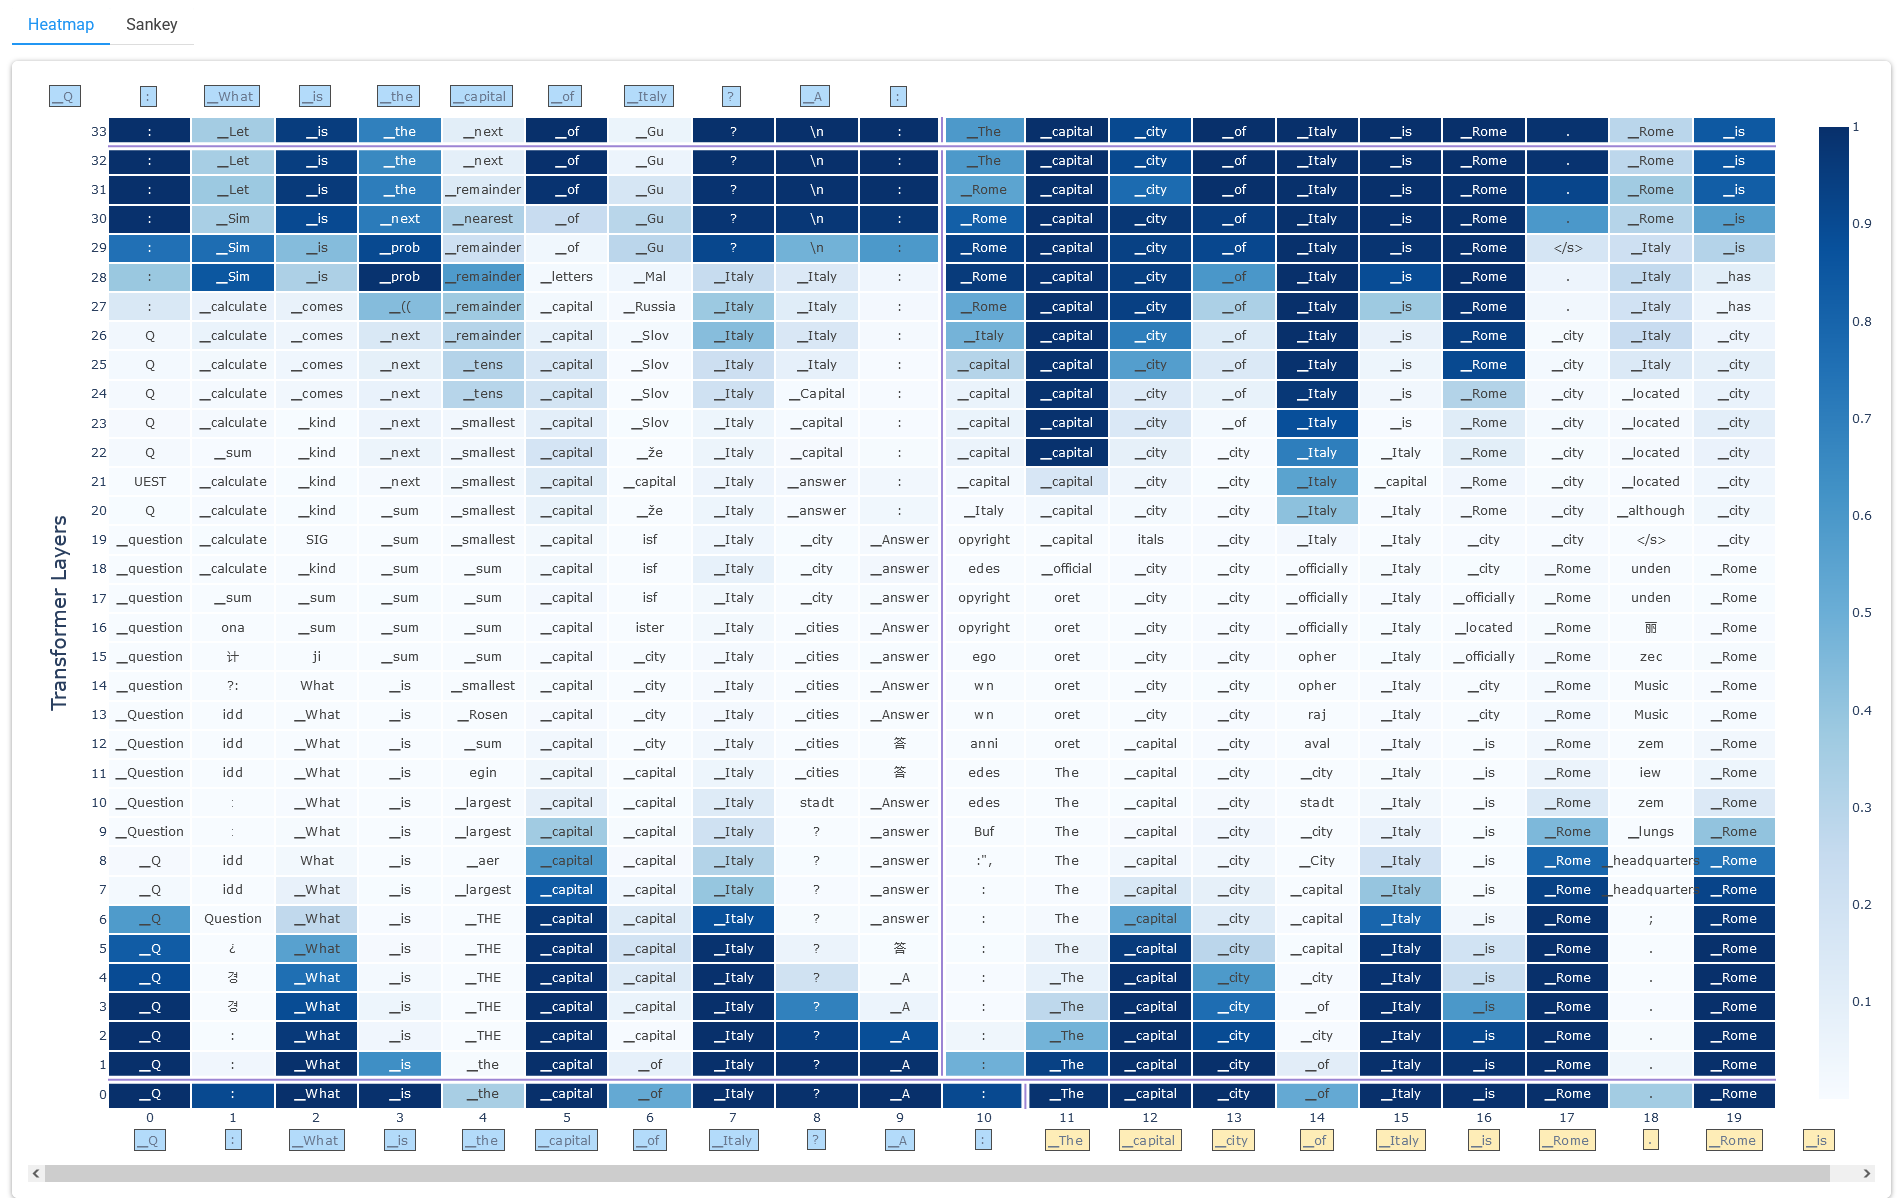
\includegraphics[width=\textwidth]{exp_intravisto_1A_heatmap.png}
    \caption[InTraVisTo's heatmap visualization given the prompt \emph{``What is the capital of Italy?''} to Mistral.]{InTraVisTo's heatmap visualization given the prompt \emph{``What is the capital of Italy?''} to Mistral, utilizing linear interpolation for decoding and probability of the argmax term for color.}
    \label{fig:exp_intravisto_1_A}
\end{figure}

\begin{figure}[t!]
    \centering
    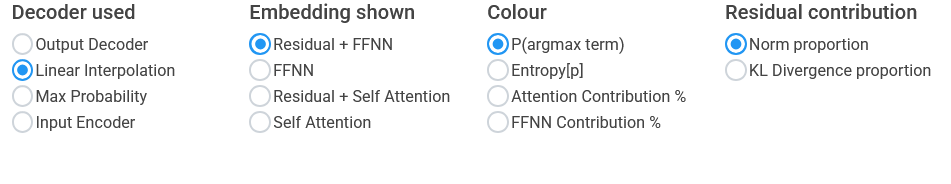
\includegraphics[width=\textwidth]{exp_intravisto_1B_selectors.png}
    \caption[Selector panel containing InTraVisTo controls.]{Selector panel containing InTraVisTo controls to set (from left to right) \emph{decoding strategy}, \emph{target embedding}, \emph{probability} to display and \emph{attribution formula} of component outputs to the residual stream.}
    \label{fig:exp_intravisto_1_B}
\end{figure}

The \emph{embedding} refers to the position of the hidden state vector to be decoded within the layer.
Therefore, by selecting different embedding positions, the user can inspect distinct subcomponents within each layer and understand which information is propagated between layers.
In order to prevent saturating the visualization with information, only a single embedding position can be visualized at any given time using the heatmap.

Conversely, the \emph{decoding strategy} choice refers to the decoding matrix employed during the decoding process of each visualized hidden state, fulfilling the role of ``perspective'' for the interpretation.
Selecting an effective decoding strategy is a nontrivial task and can be considered the key element of the vocabulary decoding approach to interpretability.
As reviewed in~\cref{ssec:related_vocab}, numerous approaches for decoding hidden states already exist in literature.
InTraVisTo's decoding operation is formalized in~\cref{eq:method_intravisto_decoding} and utilizes a user-selected decoding matrix.
In addition to immediate choices such as input embeddings or output embeddings, which are focused on providing meaningful decoding for lower and upper layers of the network respectively, InTraVisTo also offers the possibility of decoding states using interpolated and max-probability decoders, defined in~\cref{eq:method_intravisto_linear-interp,eq:method_intravisto_quadratic-interp,eq:method_intravisto_max-p}.
These novel decoding techniques are designed in order to provide users with semantically meaningful representations for every layer of the model simultaneously.

Finally, the \emph{probability selector} directly affects the quantity used to weight the color grading in the heatmap.
The four main options consist of P(argmax term), entropy, attention contribution and feedforward contribution. % chktex 36
Additionally, a secondary control labeled as ``Residual Contribution'' affects the attention and feedforward contribution options for the probability selector.
This control determines the metric used to evaluate the concept of contribution between Transformer components and the residual stream according to~\cref{eq:method_intravisto_norm-contrib,eq:method_intravisto_kl-contrib}.
The mathematical background for these selectors is discussed in detail in~\cref{sssec:method_intravisto_decoding_metrics}.

Additionally, users are provided with several secondary controls to further explore the models' generation process, as illustrated in~\cref{fig:exp_intravisto_1_C}.
For example, the `Embedding normalization' control allows users to select the type of normalization to apply to hidden states before decoding, as defined in~\cref{eq:method_intravisto_normalization}.
Another selector is dedicated to handling the strategy for decoding secondary tokens (see~\cref{sssec:method_intravisto_decoding_tokens}), offering either a `top-$5$' approach or by using the iterative decoding algorithm, as illustrated in~\cref{alg:method_intravisto_iter-dec}.
Moreover, users are given the option to exclude the column corresponding to the \emph{<start>} token from the visualization, as decoding it often does not yield meaningful results.
Furthermore, users can influence the generation process by choosing a different model from a customizable selection pool or by adjusting the number of generated tokens using the appropriate selectors.

\begin{figure}[t!]
    \centering
    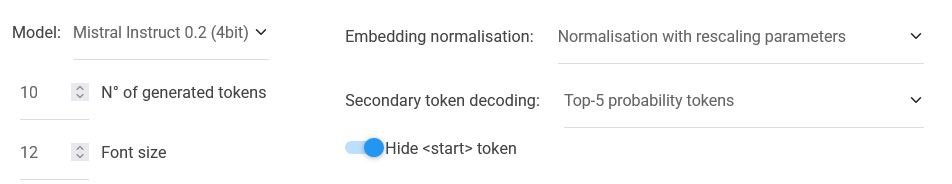
\includegraphics[width=\textwidth]{exp_intravisto_1C_controls.png}
    \caption{Selector panel containing additional generation and visualization controls for InTraVisTo.}
    \label{fig:exp_intravisto_1_C}
\end{figure}

\subsection{Flow Interface}\label{ssec:exp_intravisto_exp2}

The second visualization provided by InTraVisTo is a Sankey diagram that aims to depict the information flow through the Transformer network (\cref{fig:exp_intravisto_2_A}).

\begin{figure}[t!]
    \centering
    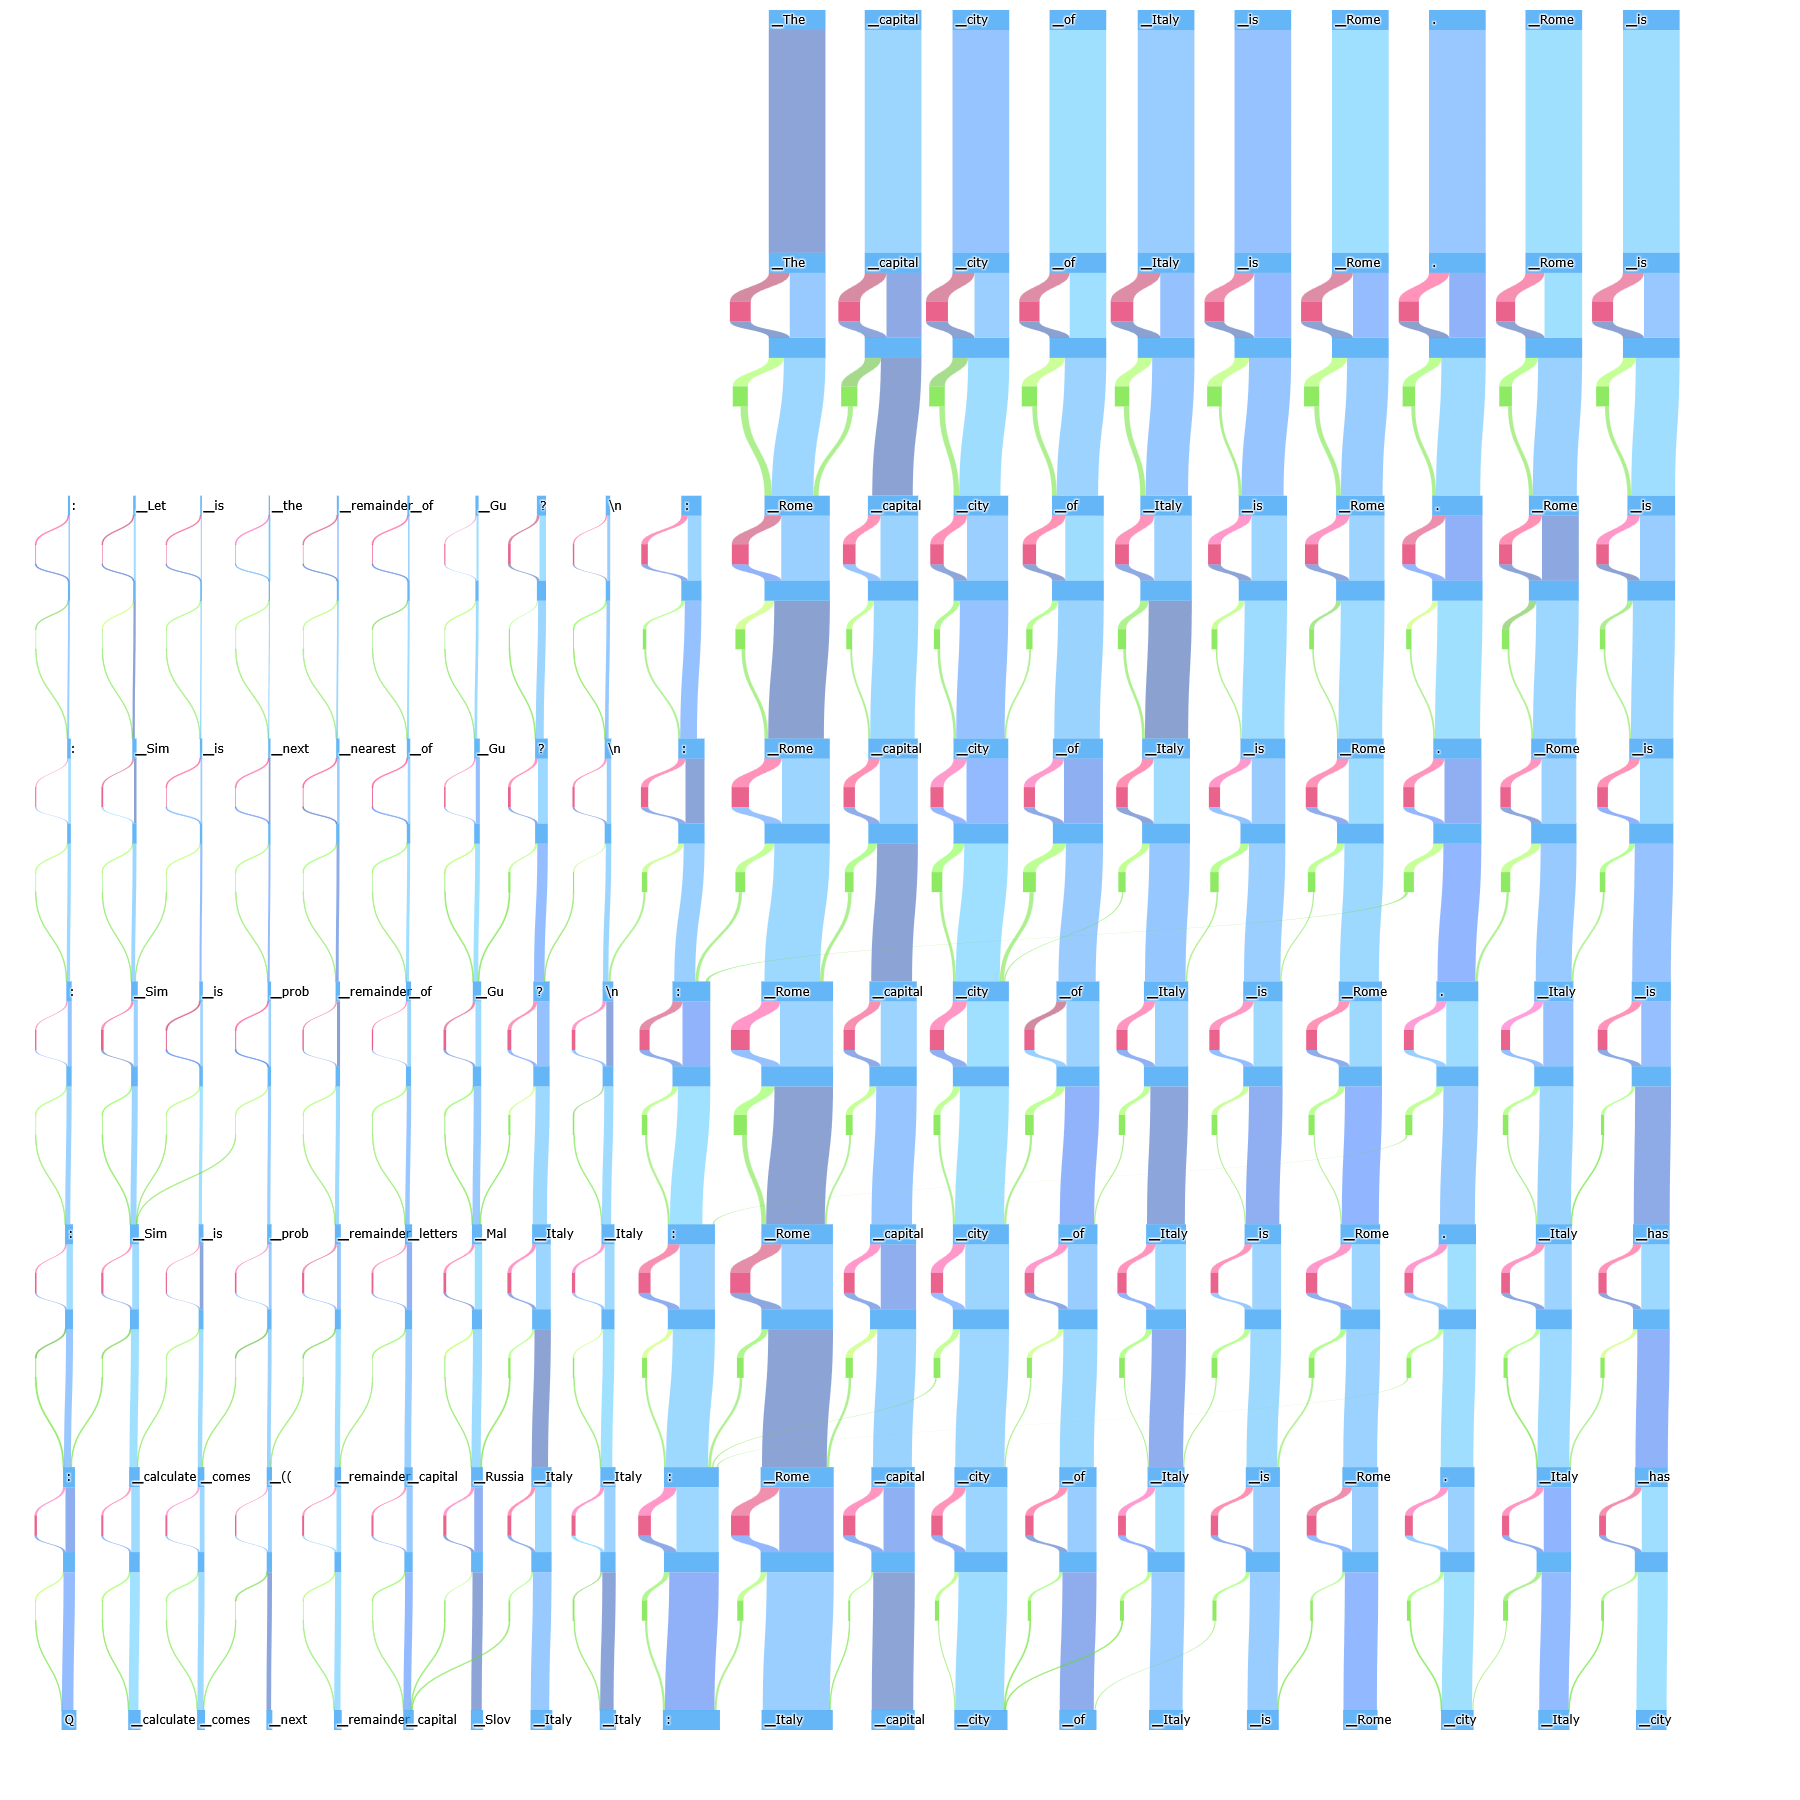
\includegraphics[width=0.9\textwidth]{exp_intravisto_2A_sankey.png}
    \caption[InTraVisTo's Sankey diagram visualization given the prompt \emph{``What is the capital of Italy?''} to Mistral.]{InTraVisTo's Sankey diagram visualization of the last 7 layers given the prompt \emph{``What is the capital of Italy?''} to Mistral, utilizing linear interpolation for decoding, showing only the top attention trace and calculating residual contributions using the norm.}
    \label{fig:exp_intravisto_2_A}
\end{figure}

Nodes in the diagram depict all the hidden states contained in each layer, visualizing each one of the four vectors referenced in~\cref{ssec:method_intravisto_decoding} at the same time.
Similarly to the heatmap visualization, nodes display the main decoding result as their label and, when hovered upon, provide additional information in the form of a pop-up tooltip containing secondary tokens.
One additional piece of information, exclusively found in the tooltip of output nodes, is the decoded difference from the previous layer.
This detail shows the primary and secondary tokens obtained from decoding the difference between the output state of the current layer with the output state of the previous layer as if it were a separate state.
The goal of this representation is trying to visualize in a human interpretable way, the information added by the current layer with respect to the previous one.

On the other hand, edges represent the amount of relevance carried by the residual stream, illustrating how various components accumulate or disperse this flow as they process information scattered throughout the model.
Being a Sankey diagram, no amount of flow is ever lost between layers, as the flow corresponding to all tokens in a horizontal section (representing a layer) always sums to $100\%$.
The flow originates from the topmost layer of nodes, and is recursively computed considering the contributions of each encountered node.
More specifically, flow computation is discussed in detail in~\cref{ssec:method_intravisto_flow} and can be formalized using~\cref{eq:method_intravisto_flows}.

When considering a new generation run, the totality of the flow is evenly split between the output nodes at the end of the Transformer stack.
However, if the user decides to inspect a specific cell in the heatmap by clicking on it, the Sankey diagram also adapts by recalculating the flow considering the corresponding node as the sole topmost node, consequently accounting for $100\%$ of the flow.
We subdivide nodes into three categories, color-coded for visualization convenience: intermediate and output nodes in blue, attention nodes in green and feedforward nodes in pink.
Moreover, flows exiting from each node inherit the color of their originating node, leading to a clear display of the main information paths and their direction.
Additionally, flows are given a further shading factor that is proportional to the KL divergence between the decoded hidden state distributions of the nodes that they connect.
This allows users to appreciate in an immediate way states that exhibit rapid changes in distribution, thus providing a better localization for possible zones of interest.

The only component that is able to redistribute the flow through various tokens is the attention node, which does so according to the attention weights computed for all preceding tokens.
Furthermore, for each aggregation node (intermediate and output), the flow contribution of the preceding nodes is computed following the ``Residual contribution'' user control mentioned in~\cref{ssec:exp_intravisto_exp1} according to~\cref{eq:method_intravisto_norm-contrib,eq:method_intravisto_kl-contrib}.

InTraVisTo is equipped with additional settings exclusively dedicated to the Sankey diagram visualization as illustrated in~\cref{fig:exp_intravisto_2_B}.
First, we provide a flag for hiding the starting token similar to the one defined in~\cref{ssec:exp_intravisto_exp1}.
However, in the Sankey's case it comes with an additional control that allows users to reapport the hidden flow to remaining nodes, meaning that the values of hidden flows are set to $0$ and the missing percentage is redistributed to visible tokens.
Another important setting is the ``Attention highlight'', which controls the criteria for highlighting attention traces, affecting the number of visible flows related to each attention node.
Users can choose between visualizing all flows, only the top-$k$ flows (based on attention weights), displaying only flows with a corresponding attention weight greater than a certain threshold, or showing no flows at all.
Other graphic-oriented options allow users to remove node labels for nodes that do not constitute the output of a layer, adjust the scale of the diagram and select the depth of the visualization by choosing the number of visible layers.

\begin{figure}[t!]
    \centering
    
\includegraphics[width=\textwidth]{exp_intravisto_2B_controls.png}
    \caption{Selector panel containing specific visualization controls related to InTraVisTo's Sankey diagram.}
    \label{fig:exp_intravisto_2_B}
\end{figure}

\subsection{Dynamically Changing the Network}\label{ssec:exp_intravisto_exp3}

InTraVisTo is designed as an interactive tool, and embedding injection is another feature intended to enhance understanding of the internal workings of Transformers.
As formalized in~\cref{ssec:method_intravisto_injection}, injection involves substituting a hidden state with a custom embedding representation, forcing the model to adjust its behavior based on the injected information.
Injections can be performed by clicking on a cell in the grid-layout heatmap; this actions opens a pop-up menu (\cref{fig:exp_intravisto_3_A}) associated with the cell, which then prompts the user for the following information:
\begin{itemize}
    \item A string of text with the purpose of being encoded into an embedding representation and injected inside the selected hidden state.
The application automatically converts the string into an embedding using the inverse transformation of the chosen decoder.
If the string contains multiple tokens, then all encoded representations are averaged to obtain a single embedding in accordance to~\cref{eq:method_intravisto_emb-avg}.
    \item The injection technique, which controls how the new embedding is integrated into the preexisting state, as specified in~\cref{eq:method_intravisto_inj_complete,eq:method_intravisto_inj_main}.
    \item The position of the injection inside the selected layer, allowing users to inject embeddings in every position without changing the heatmap visualization.
    \item The decoding technique used to interpret the aforementioned string of text.
    \item The option to normalize the injected embedding according to the selected injection technique.
\end{itemize}

\begin{figure}[t!]
    \centering
    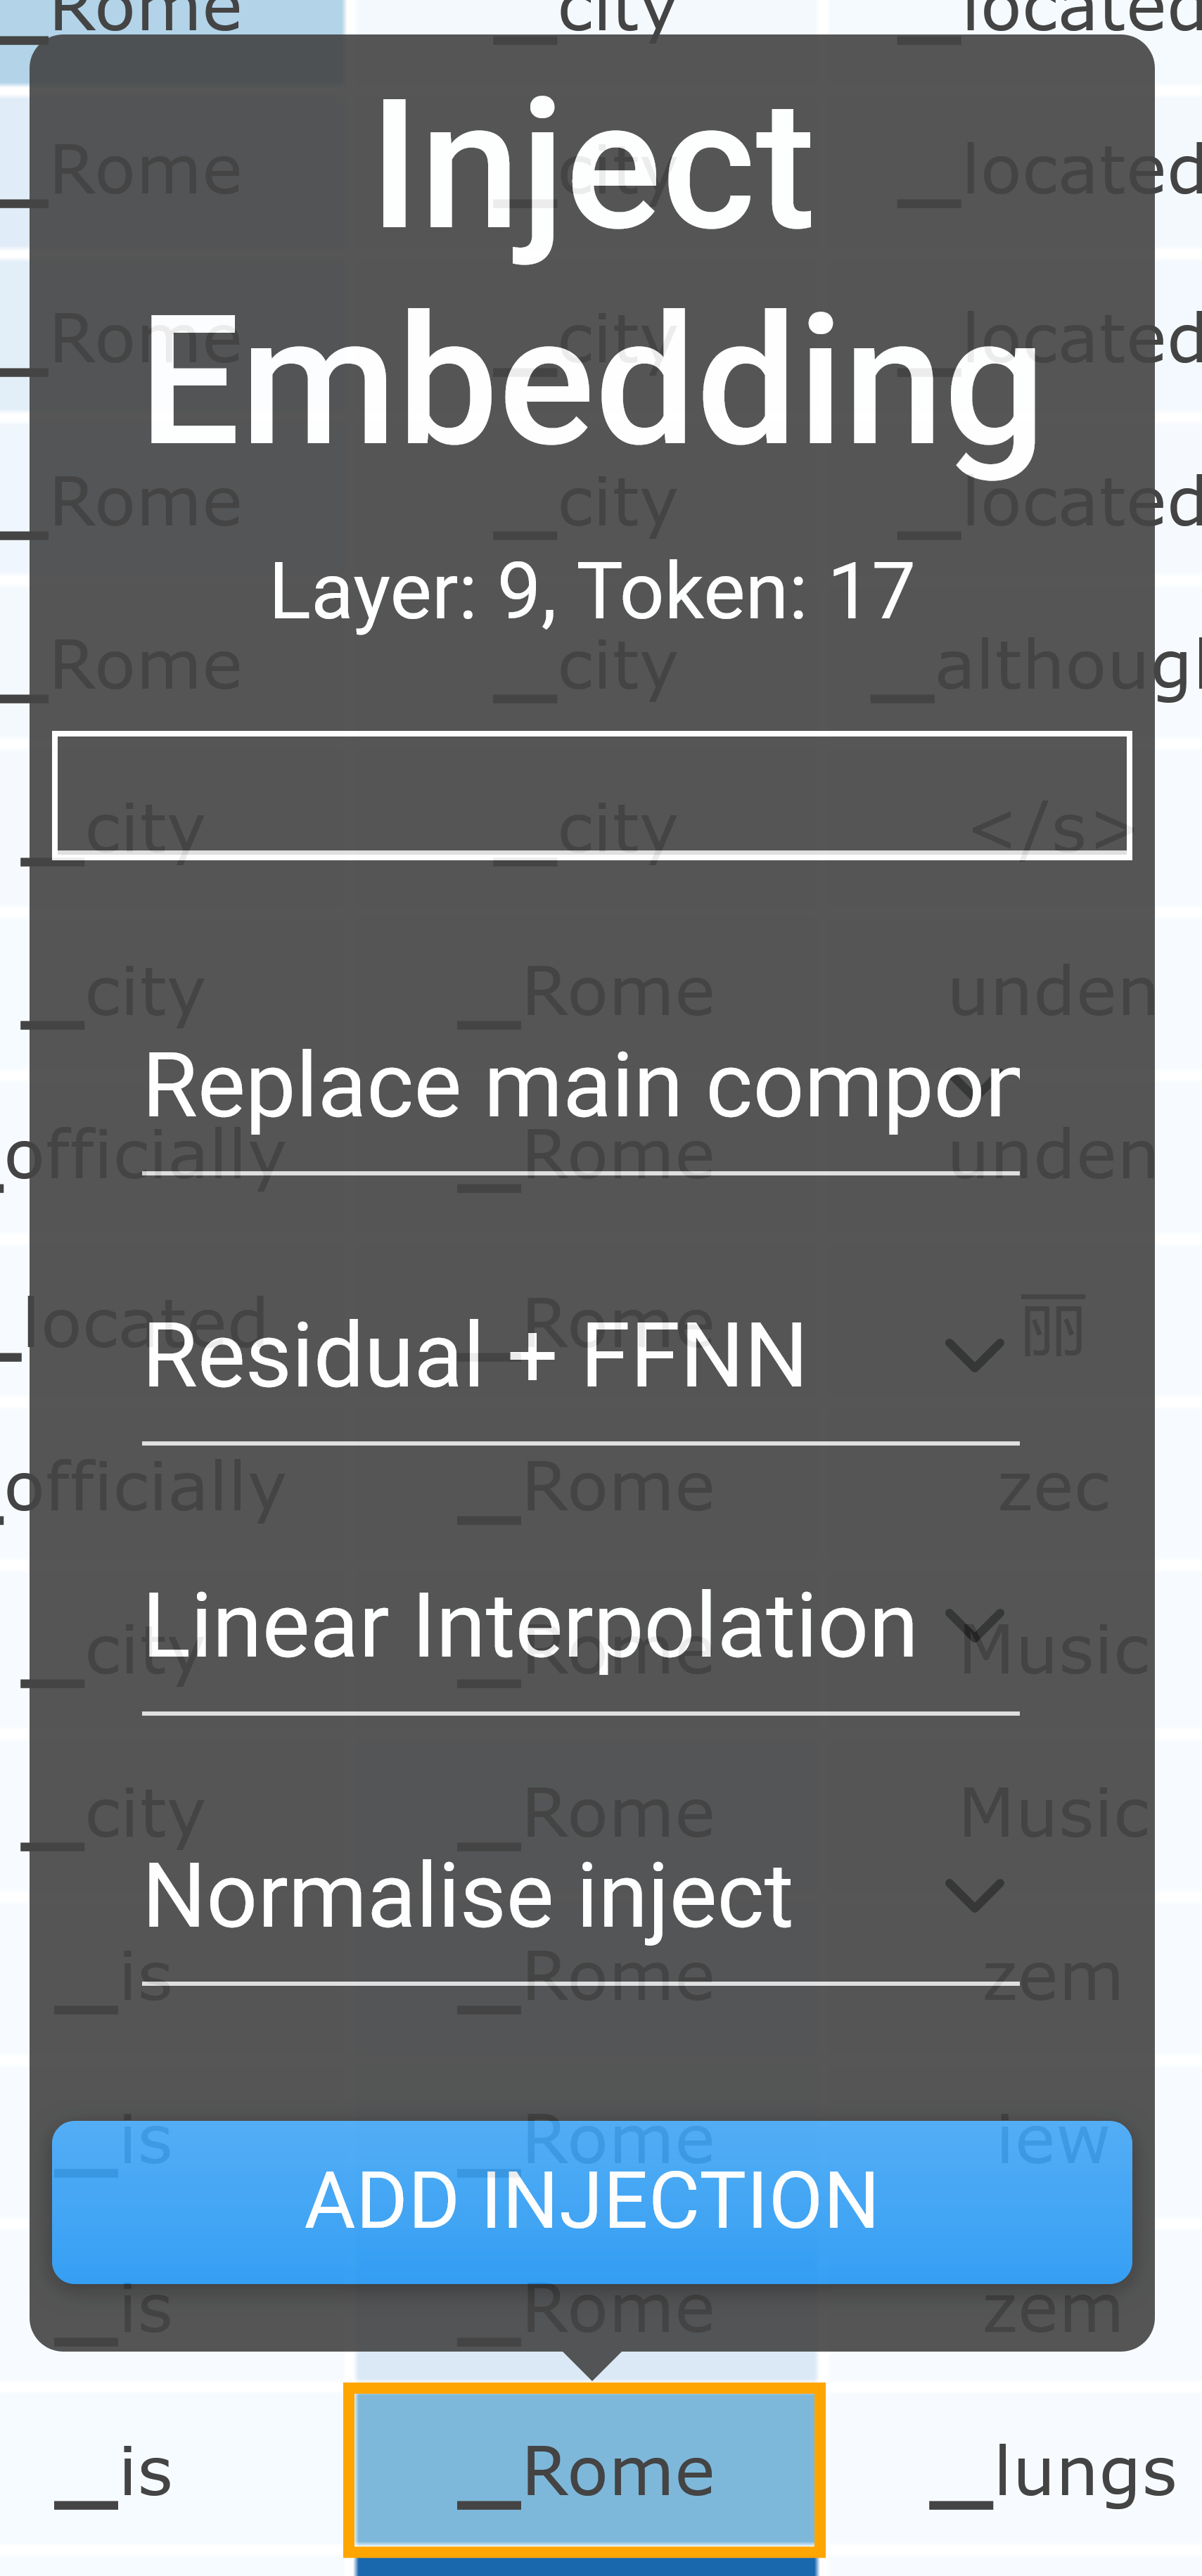
\includegraphics[width=0.25\textwidth]{exp_intravisto_3A_popup.png}
    \caption[InTraVisTo's pop-up menu utilized for injections.]{InTraVisTo's pop-up menu utilized for injections, containing an input box for specifying the injection prompt and selectors for \emph{injection technique}, \emph{injection position}, \emph{decoding technique} and eventual \emph{normalization} options.}
    \label{fig:exp_intravisto_3_A}
\end{figure}

Once a valid injection is compiled and added, a small card summarizing the injection is created and displayed in a dedicated section at the top of the interface.
This operation triggers an immediate reload of the current generated result by the model to incorporate the newly defined injection.
When the heatmap visualization presents the result of a generation process that included an injection, the corresponding cell location is highlighted in \emph{green}.
Injections can be removed at any time from the generation process by pressing the appropriate `X' button on their card.
The standard layout of injection cards is shown in~\cref{fig:exp_intravisto_3_B}.

\begin{figure}[t!]
    \centering
    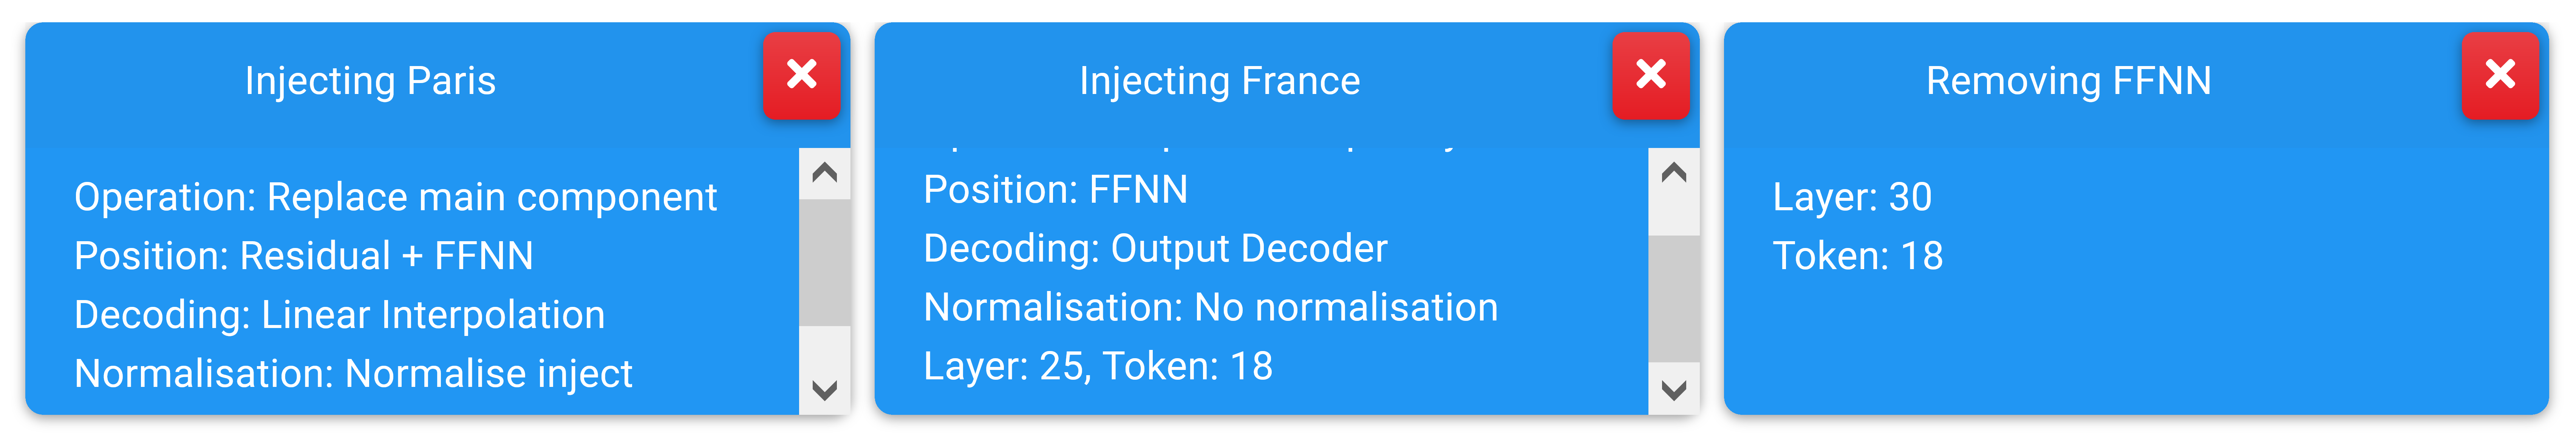
\includegraphics[width=0.7\textwidth]{exp_intravisto_3B_cards.png}
    \caption[Injection and ablation cards containing summaries of information that will be used to affect the model generation process.]{Two injection cards (left and center) and an ablation card (right) containing summaries of information that will be used to affect the model generation process.}
    \label{fig:exp_intravisto_3_B}
\end{figure}

As mentioned earlier in~\cref{ssec:exp_intravisto_exp1}, it is also possible to perform injections in the Sankey diagram by clicking on any visible node, triggering the same injection pop-up menu described above.
If the chosen node corresponds to a feed-forward or an attention node, there is an additional option that allows the user to remove the node, performing an ablation.
Ablations are processed similarly to injections; a card is created in the top section of the interface (\cref{fig:exp_intravisto_3_B}), and the generation process is repeated to incorporate the selected changes.
Removing a node is handled by nullifying its contribution to the residual, therefore its hidden state is still properly decoded and can be analyzed from the heatmap, but does not influence the rest of the model.
As with injections, ablations are highlighted in \emph{red} within the heatmap visualization.

\subsection{Case Study: Utilizing InTraVisTo to Inspect the Internal Behavior of Models}\label{ssec:exp_intravisto_exp4}

For this experiment we submit various prompts to a selection of different models and explore specific aspects of the extracted internal representations and information flows utilizing InTraVisTo.

It is a well known fact that current general-purpose language models have exhibited poor overall performance on tasks involving the use of numbers and mathematical operators.
Consequently, significant focus is placed on this particular topic, with some prompts being specifically set up to induce models to perform computations of numerical nature.
Nonetheless, we explore a great variety of prompts and gather valuable insight from different perspectives, with the overall goal of demonstrating the potential of the proposed tool.

\subsubsection{Experimental Setup}\label{sssec:exp_intravisto_exp4_expset}

By directly experimenting with the proposed tool, we establish a basic workflow that enables researchers to ultimately collect new insights about how LLMs generate tokens in a layer-by-layer fashion.
The first step consists in exploring the secondary representations of internal states in order to find additional information relevant for the task at hand, since the model may encode such details in the latent dimensions of hidden states alongside the main token, utilizing the residual stream as a communication channel between modules.

Based on the information previously gathered, the next step is to examine the cumulative influence on hidden states of interest generated by the model.
This can be achieved by utilizing the Sankey diagram visualization of InTraVisTo, piecing together the contribution of tokens and components that had a major role in the creation of certain intermediate states, enabling the formation of conjectures about the model's inner workings.

Finally, by acting upon these conjectures using the state injection and component ablation tools provided by InTraVisTo, it is possible to generate new knowledge by identifying the root causes that determine certain internal behaviors manifested in the preliminary inspection.
This knowledge can be further generalized by replicating the experiments on multiple models and observing possible similar mechanics at play, even between different architectures.

It is important to note that not every included discovery was made using the suggested workflow, since it only represents a general guideline to our approach.
A modest portion of our findings includes observed facts emerged from the thorough use of InTraVisTo, collected and formalized as empiric observations on the analyzed models.

\subsubsection{Dataset}

The dataset employed for this experiment consists of a small set of curated examples used to elicit model predictions in order to observe meaningful internal states.
A significant portion of the proposed prompts involves solving tasks of mathematical and numerical nature due to their simplicity and tendency towards eliciting erroneous answers from models.
This increase in the likeness of reasoning errors in LLMs for numerical tasks is often associated with \emph{attention glitches}: minor errors propagated throughout the attention pattern in the model~\cite{liu2023}.

The following constitutes a comprehensive list containing all main prompts used for visualizations and explorations in the current experiment.

\begin{multicols}{2}
    \begin{itemize}
        \item \emph{`What is the capital of Italy?'}
        \item \emph{`Write numbers in reverse order. Number: 13843234 Reverse:'}
        \item \emph{`10000000 + 1 ='}
        \item \emph{`1357 + 2291 ='}
        \item \emph{`15984 - 1 ='}
        \item \emph{`124101 - 4 ='}
        \item \emph{`124101 * 3 ='}
    \end{itemize}
\end{multicols}

\subsubsection{Models}

For the sake of our analysis we propose a limited number of models to be analyzed through InTraVisTo.
In particular, we consider the $4$-bit quantized versions of Mistral 7B instruct v0.2~\cite{jiang2023}, Llama 2 7B~\cite{touvron2023} and the full unquantized version of GPT-2~\cite{radford2019}.
However, the application has been developed with generality in mind, thus it can be deployed in such a way to include most popular model architectures available on Hugging Face~\cite{wolf2020}.

A key aspect of InTraVisTo is the inspection and modification of models' hidden states.
Unfortunately, under normal circumstances, only a small fraction of these states is made readily accessible by the standard Hugging Face Transformers library~\cite{wolf2020}, and the method for accessing internal components varies between model architectures and providers.
In order to obtain a comprehensive perspective of Transformer architectures, we utilize the \emph{Transformers-wrappers} framework\footnotemark: an open-source Python library initially developed by Vincenzo Scotti with the goal of exposing a uniform and extensible interface for Transformer models, while retaining a standardized internal structure for models provided by Hugging Face Transformers.
Specifically, we leverage the state inspection and API standardization capabilities offered by the library, and we contribute to the codebase by designing an extensible framework that supports the injection and ablation techniques utilized in InTraVisTo.
\footnotetext{\rlap{\url{https://github.com/vincenzo-scotti/transformer_wrappers}}}

\subsubsection{Results}

One of the earliest discoveries made via InTraVisTo is the fact that models which employ dedicated tokens for each digit, when asked to perform arithmetic operations, happen to represent decimal positional information along with digits of the result.
For example, the number $1\,492$ could be represented by having $1$ + ``thousand'', $4$ + ``hundred'', $9$ + ``ninety'' and $2$.
This was initially discovered through the unique usage of the iterative decoding technique specified in~\cref{alg:method_intravisto_iter-dec} to inspect secondary decodings of internal states, although it can also be observed in certain primary decodings where the `decimal term' interpretation takes precedence over the digit one.
We speculate that models intentionally use this technique to keep track of the current decimal position of the result while performing arithmetic operations.
This pattern can also be occasionally spotted in the reverse order as seen in~\cref{fig:exp_intravisto_4_A}, meaning that the model starts assigning decimal markers to the most significant digit, in what can be thought to be an attempt to circumvent the constraints entailed by carry operations.
Some relevant examples of decimal markers include:
\begin{itemize}
    \item \texttt{\_hundred}, \texttt{\_hundreds}, \begin{CJK}{UTF8}{goth}百\end{CJK} and \texttt{\_century} being used to indicate hundreds;
    \item \texttt{\_thousand} and \texttt{\_thousands} being used to indicate thousands;
    \item \texttt{\_thousands} and \begin{CJK}{UTF8}{goth}万\end{CJK} to indicate tens of thousands;
    \item \texttt{\_million} to indicate millions.
\end{itemize}

\begin{figure}[t!]
    \centering
    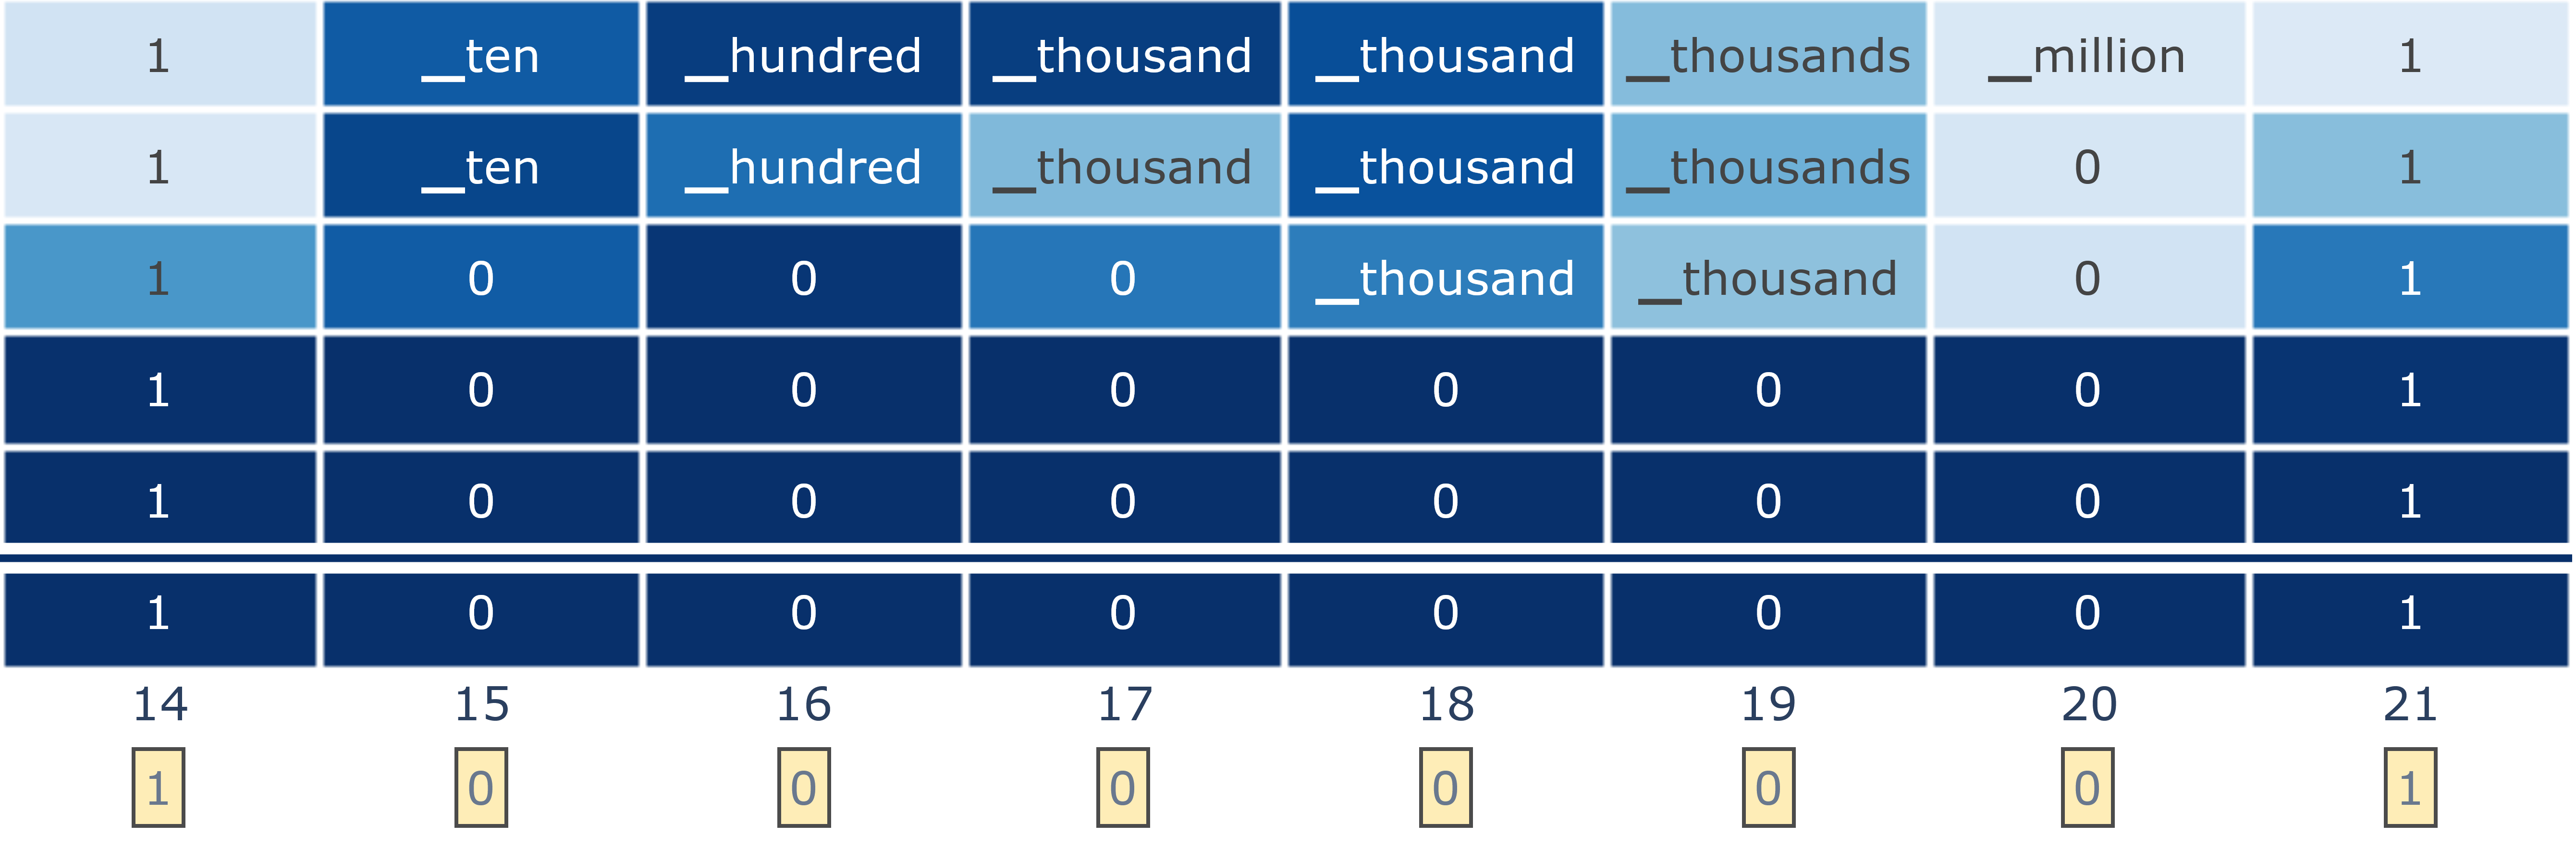
\includegraphics[width=0.8\textwidth]{exp_intravisto_4A_decimal.png}
    \caption[InTraVisTo heatmap visualization given the prompt \emph{``10000000 + 1 =''} to Llama 2.]{InTraVisTo heatmap visualization given the prompt \emph{``10000000 + 1 =''} to Llama 2, highlighting the use of progressive decimal markers in the residual stream representations.}
    \label{fig:exp_intravisto_4_A}
\end{figure}

Other interesting representations of numbers can be noticed by directly analyzing single instances of numerical tokens and observing their alternative representations as in~\cref{fig:exp_intravisto_4_B}.
For example:
\begin{itemize}
    \item Using month names such as ``July'' and ``February'' to represent single digit numbers such as $7$ and $2$ respectively (\cref{fig:exp_intravisto_4_B3});
    \item Using Roman numerals to represent single-digit numbers (\cref{fig:exp_intravisto_4_B2});
    \item Addressing numbers via plain text representations in English and other languages (\cref{fig:exp_intravisto_4_B1,fig:exp_intravisto_4_B2});
    \item Identifying the number $7$ with the token \texttt{\_lucky} (\cref{fig:exp_intravisto_4_B4}).
\end{itemize}

\begin{figure}[t!]
    \centering
    \begingroup
    \captionsetup{width=0.8\textwidth/2}
    \subfloat[Mistral addressing the digit $8$ via text representations.\label{fig:exp_intravisto_4_B1}]{%
        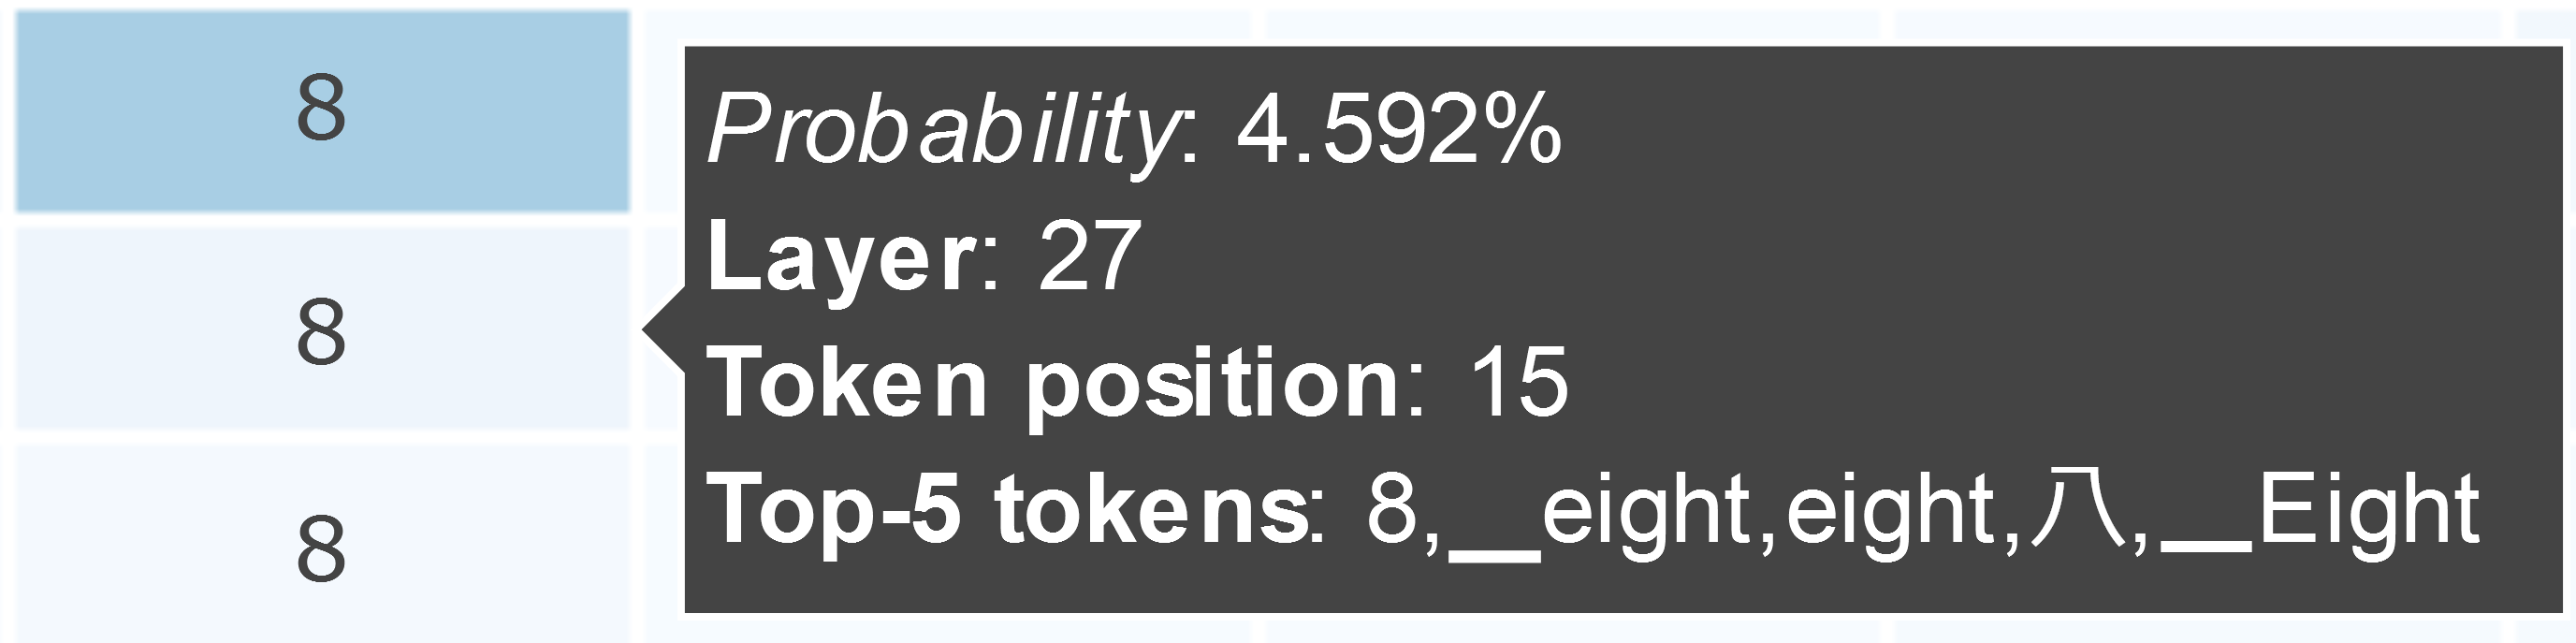
\includegraphics[width=0.5\textwidth]{exp_intravisto_4B_eight.png}%
    }%
    \subfloat[Llama 2 addressing the digit $9$ via text and alternate representations, including the Roman numeral ``IX''.\label{fig:exp_intravisto_4_B2}]{%
        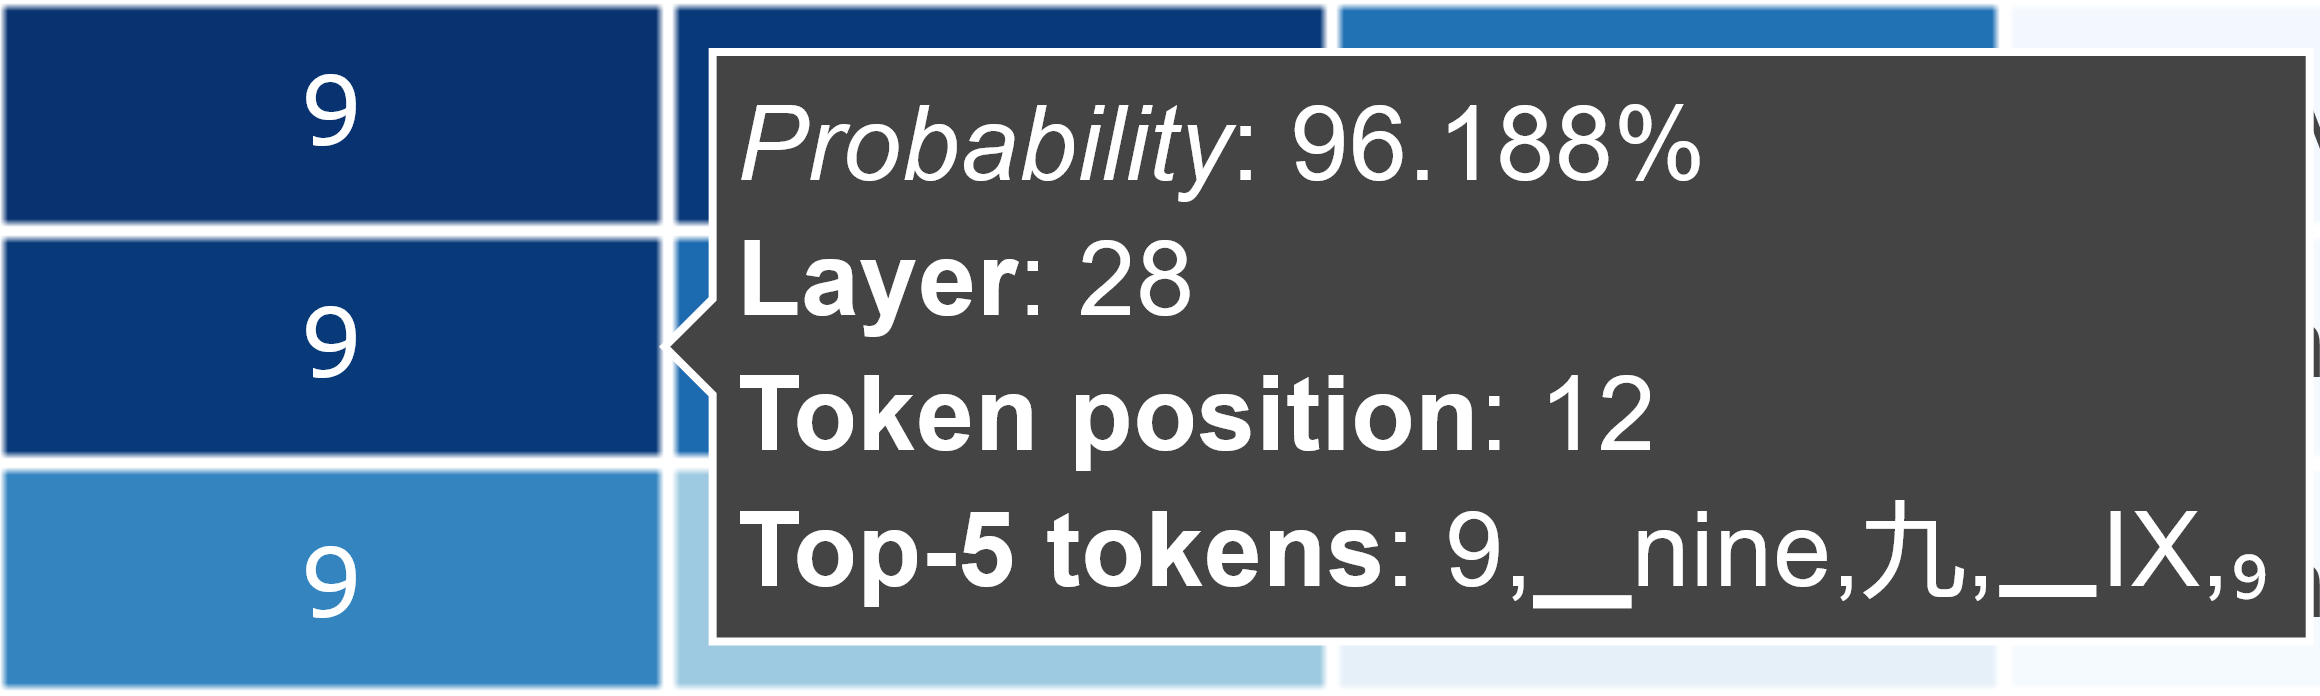
\includegraphics[width=0.4\textwidth]{exp_intravisto_4B_roman.png}%
    }%
    \quad
    \subfloat[Llama 2 addressing the digit $7$ via text representations and with the name of the corresponding month of the year: ``July''.\label{fig:exp_intravisto_4_B3}]{%
        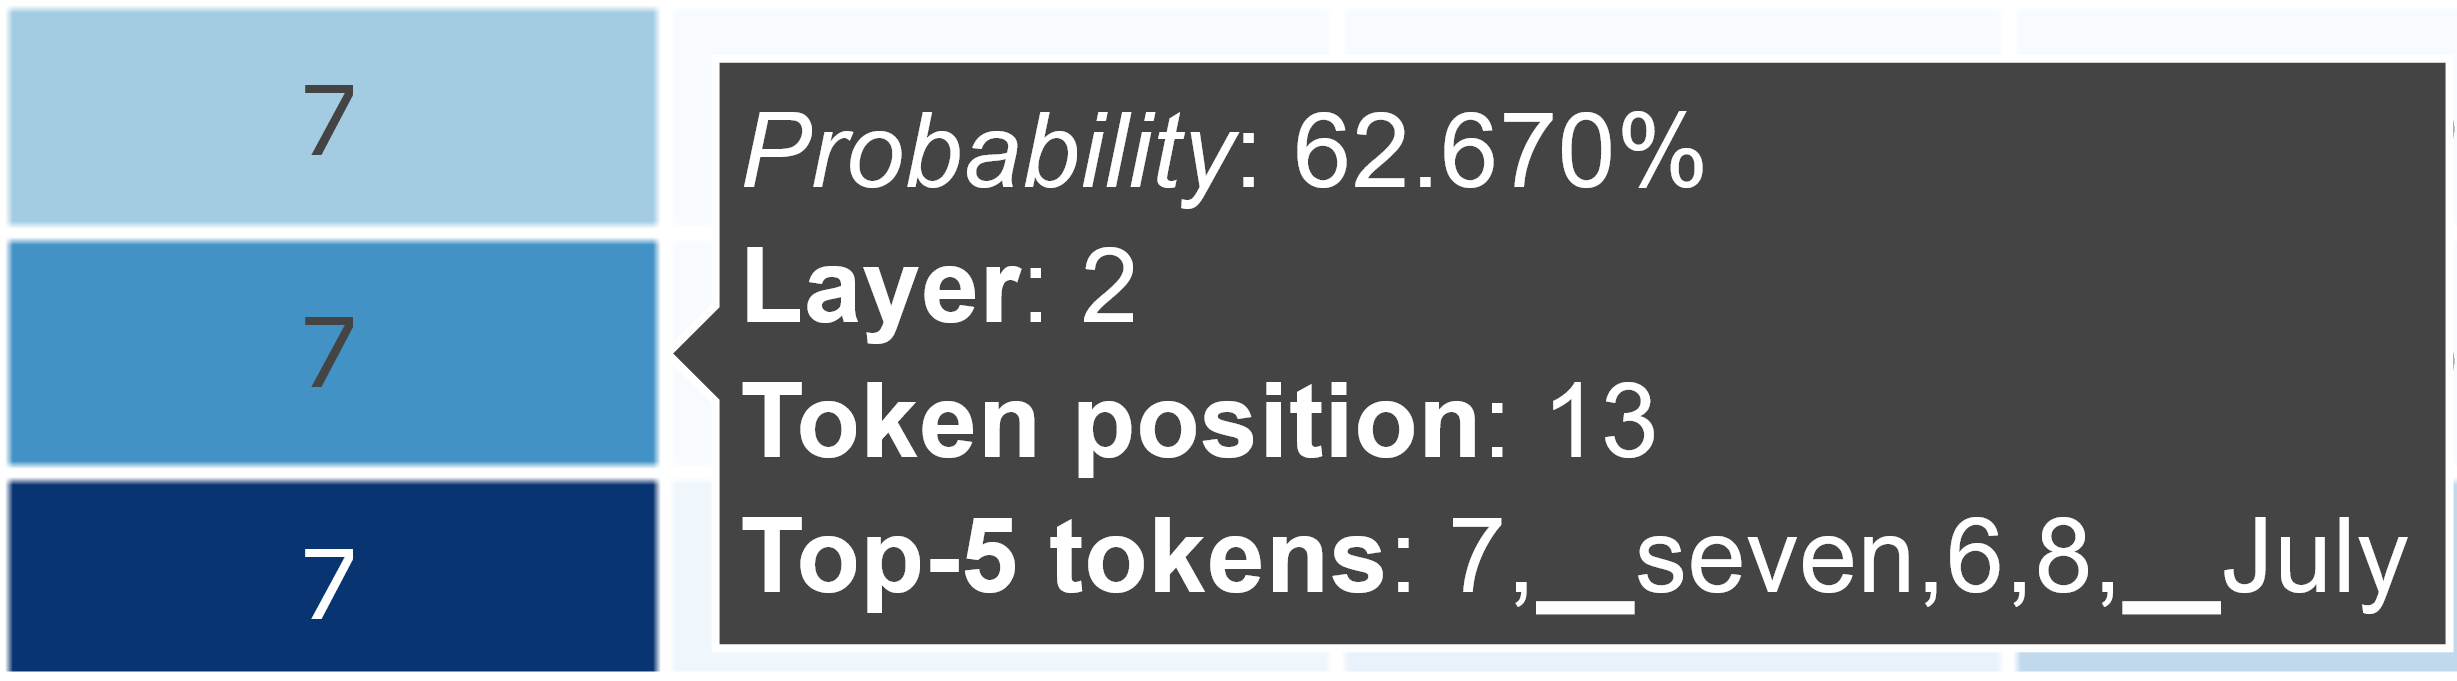
\includegraphics[width=0.45\textwidth]{exp_intravisto_4B_month.png}%
    }%
    \subfloat[Mistral addressing the digit $7$ with the token \texttt{\_lucky}.\label{fig:exp_intravisto_4_B4}]{
        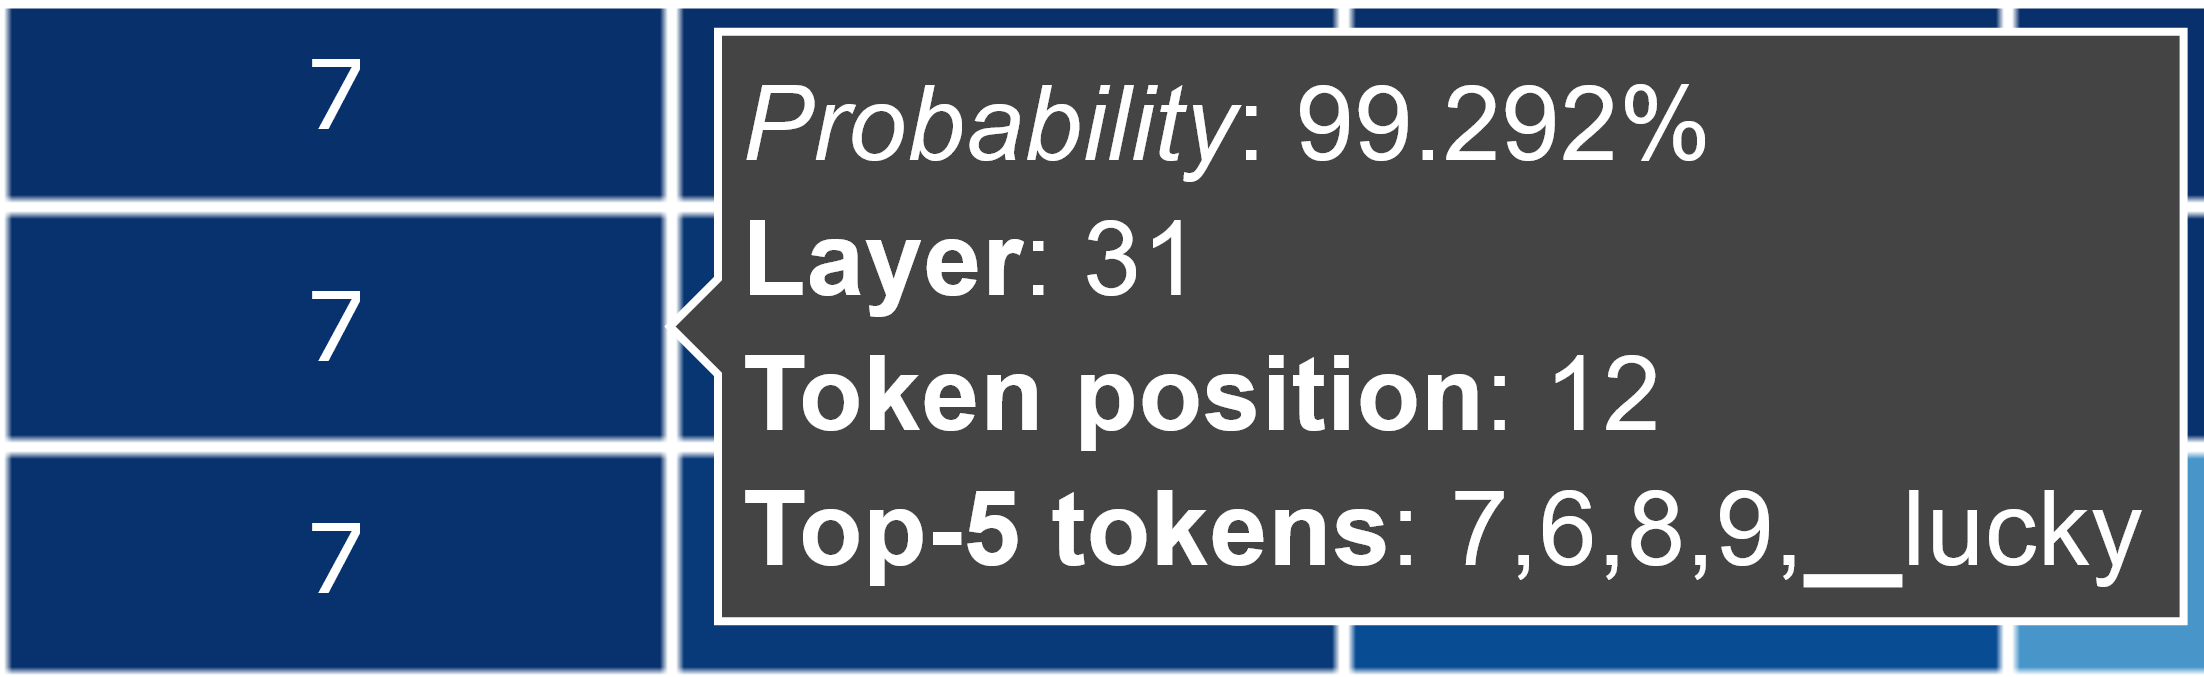
\includegraphics[width=0.4\textwidth]{exp_intravisto_4B_lucky.png}
    }%
    \endgroup
    \caption[InTraVisTo heatmap visualization for various hidden states.]{InTraVisTo heatmap visualization for various hidden states, highlighting the alternative token characterizations emerging from secondary representation obtained via iterative and top-$5$ decoding.}
    \label{fig:exp_intravisto_4_B}
\end{figure}

Alternatively, we can also perform a complete analysis over a specific query, for example \emph{``What is the capital of Italy?''}, to which the model should answer \emph{`Rome'}.
By observing the heatmap in~\cref{fig:exp_intravisto_4_C1} we can see that the model reaches the correct answer at the first generated token by gradually encoding \emph{`city'}, \emph{`capital'} and finally \emph{`Rome'} into the embeddings.
However, in the final layer, the output shifts to the determiner \emph{`The'} to produce a more formal response incorporating the original question's formulation into the answer.
In addition, by observing the Sankey diagram shown in~\cref{fig:exp_intravisto_4_C2}, it is possible to notice that during the generation process of the actual occurrence of \emph{`Rome'} at position $16$, the model collects a significant amount of attention directly from the first generated token mentioned beforehand.

\begin{figure}[tp!]
    \centering
    \subfloat[Heatmap visualization calling attention to the first generated token generative process on the left.\label{fig:exp_intravisto_4_C1}]{%
        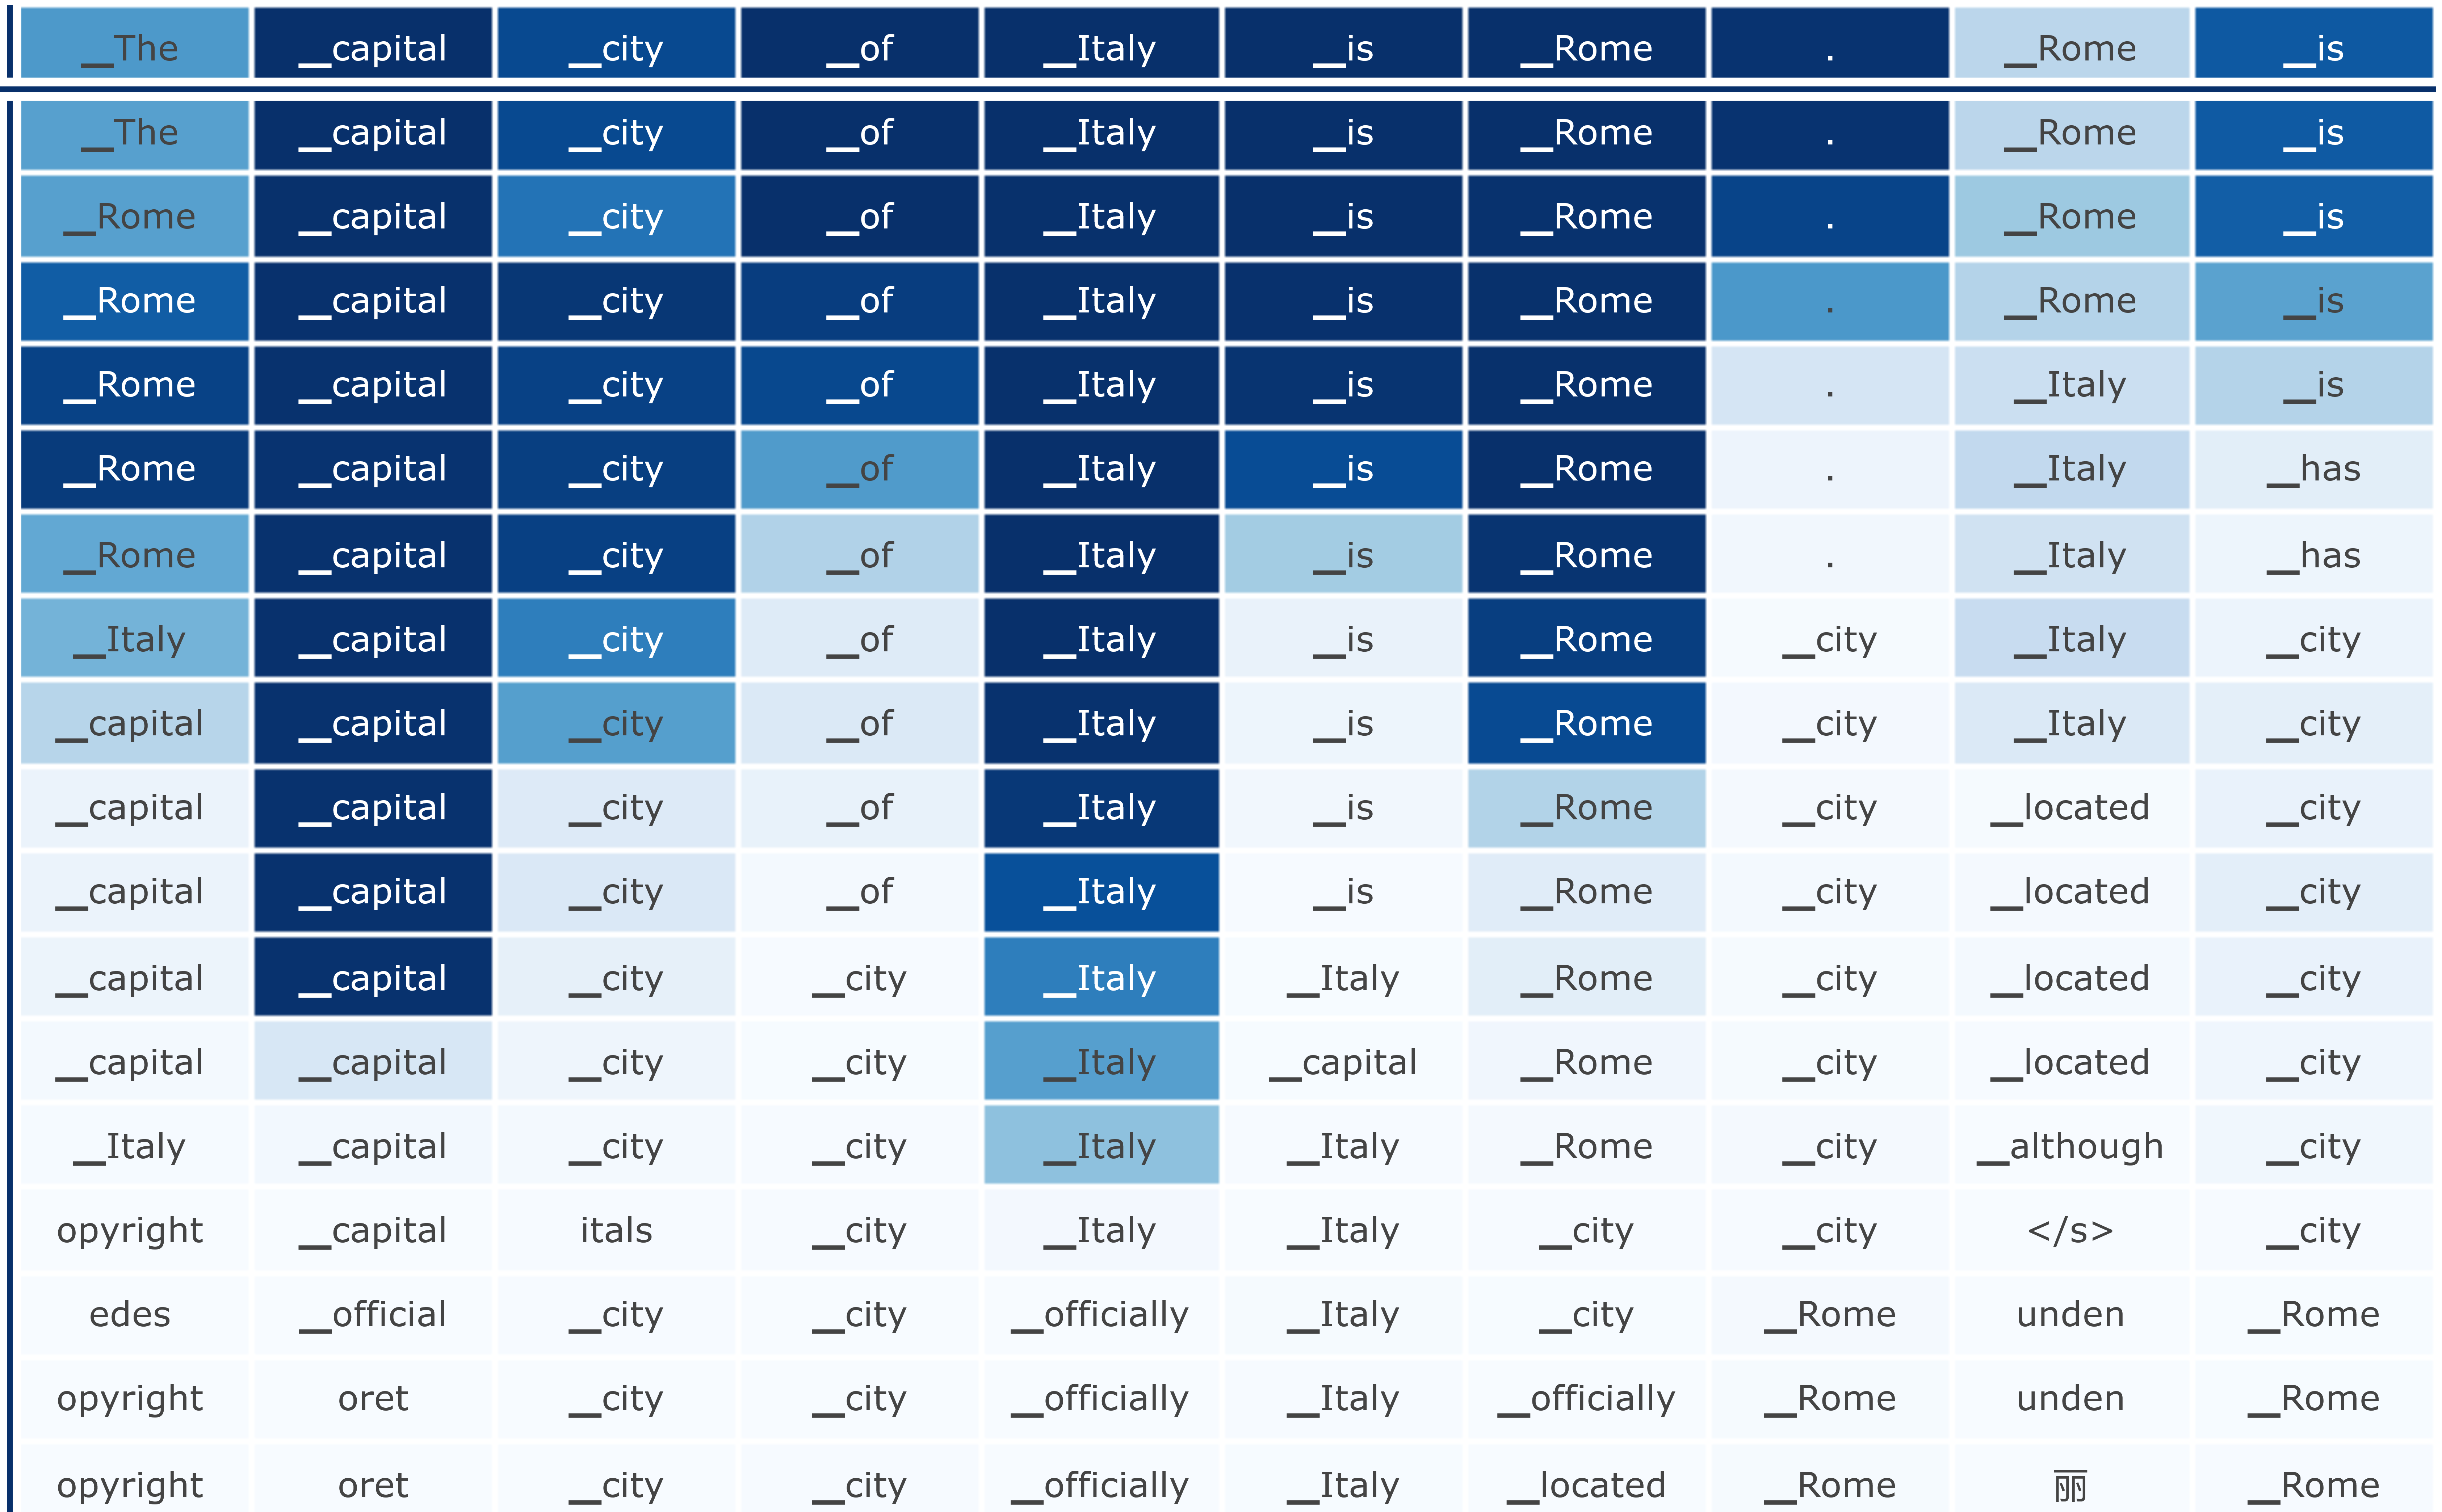
\includegraphics[width=0.7\textwidth]{exp_intravisto_4C_heatmap.png}%
    }%
    \quad
    \subfloat[Sankey diagram visualization computing flow starting from the $16$th token at layer $32$.\label{fig:exp_intravisto_4_C2}]{%
        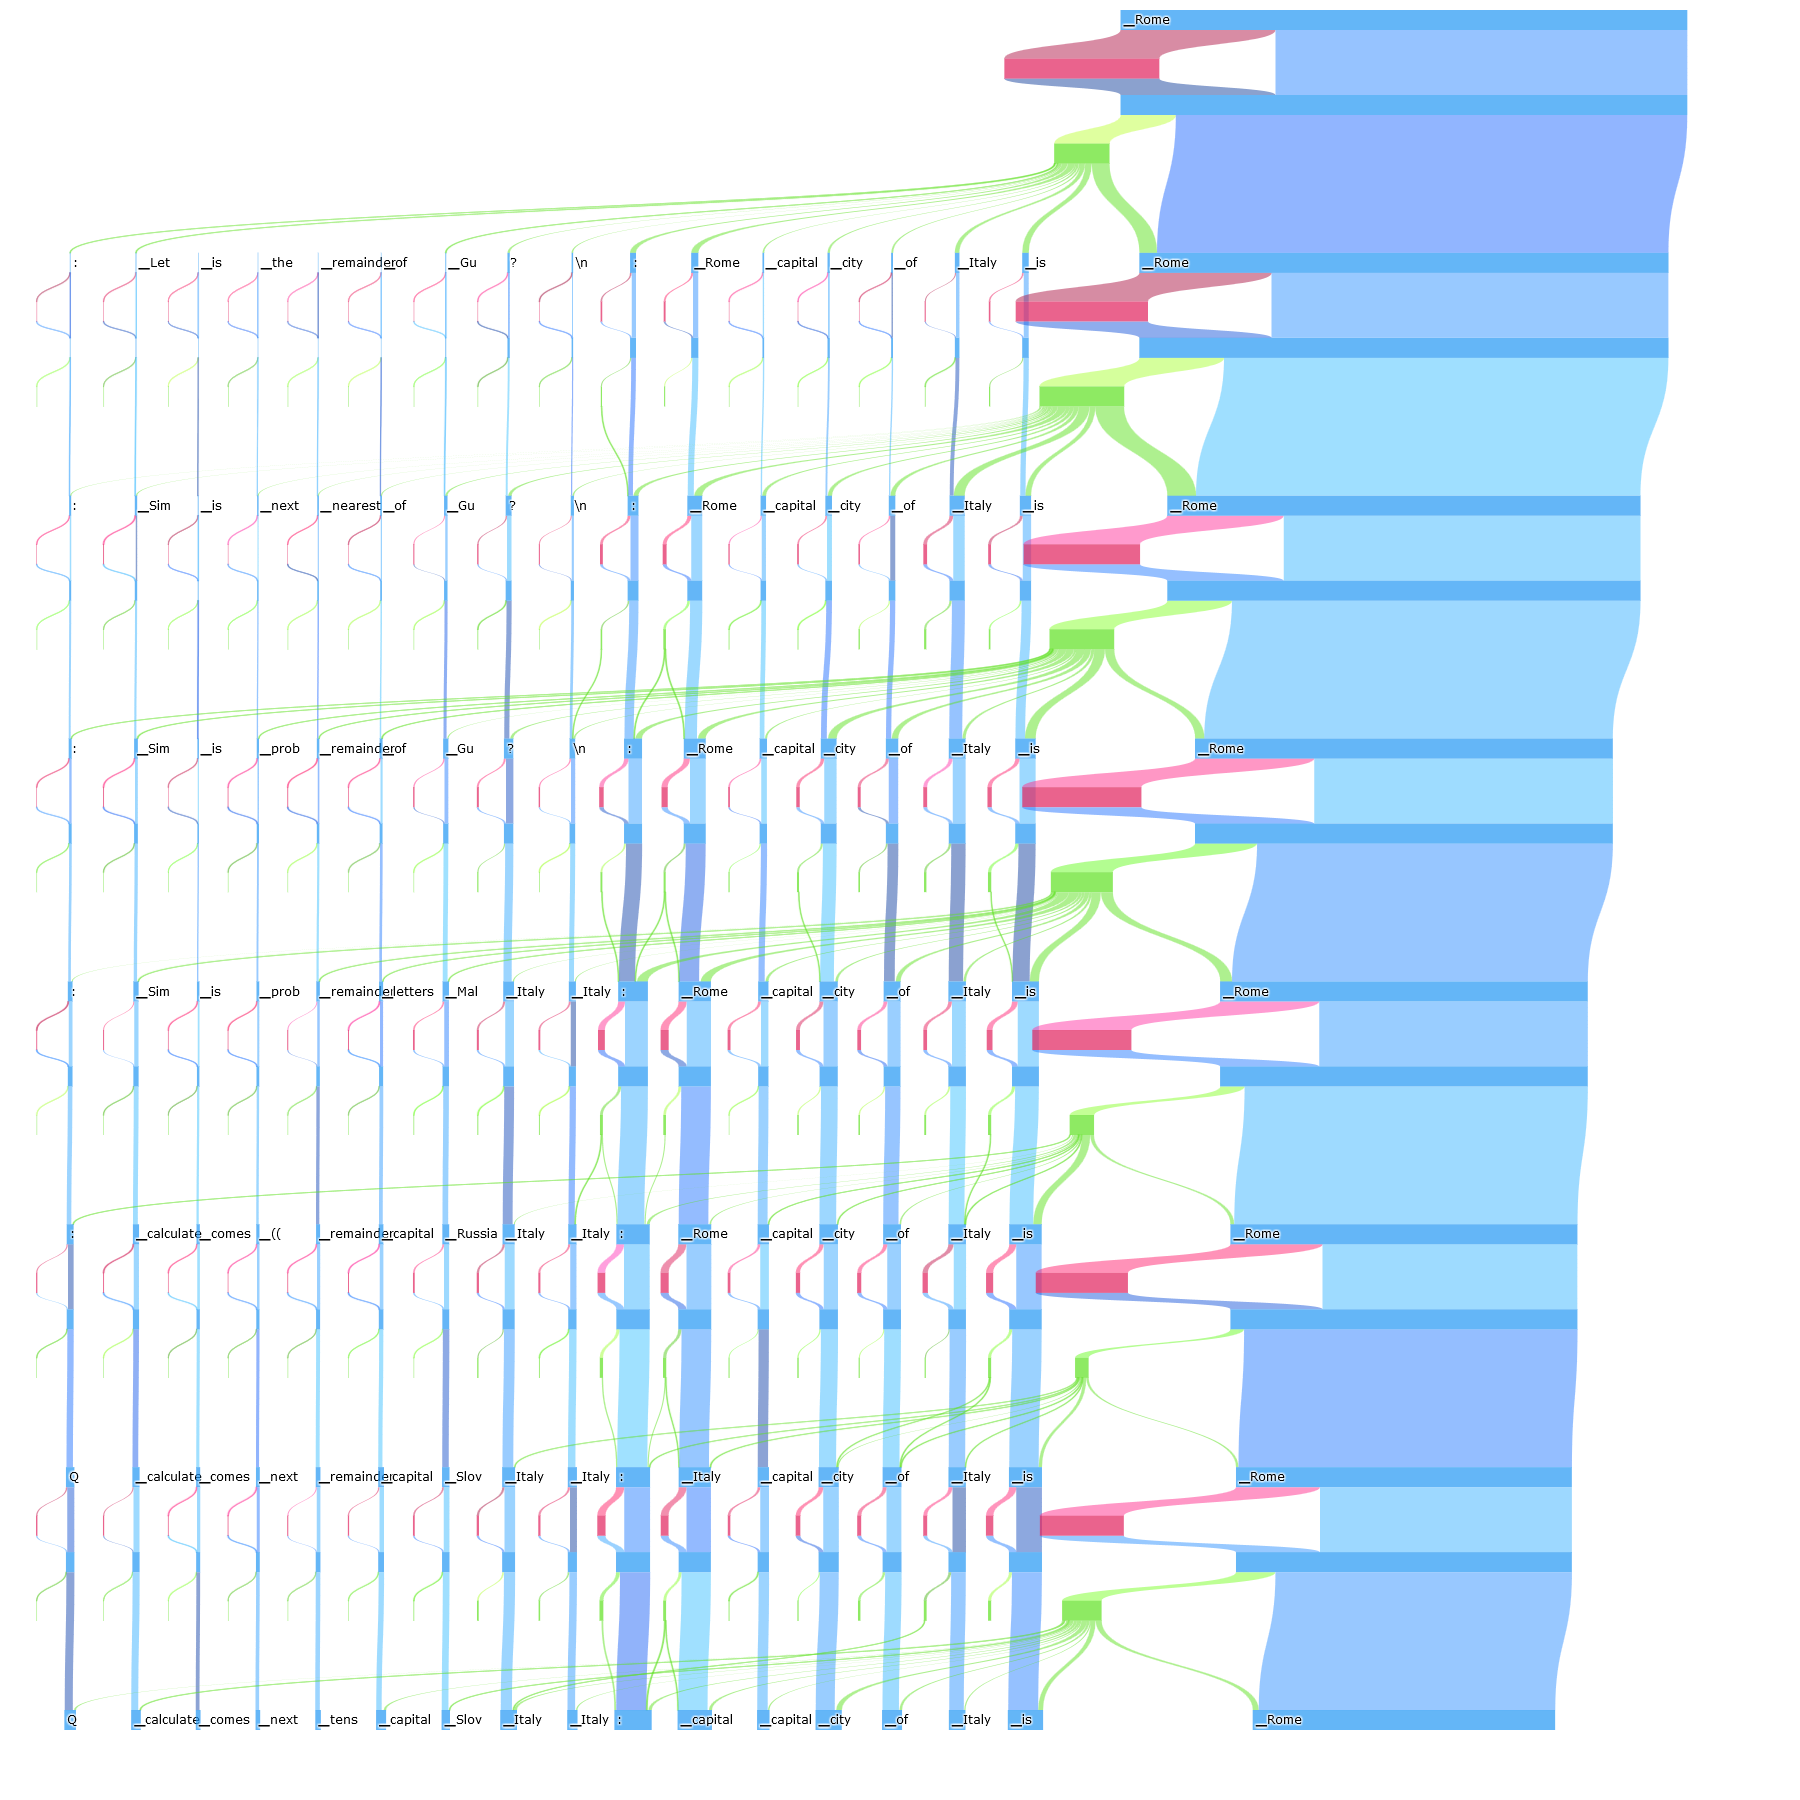
\includegraphics[width=0.7\textwidth]{exp_intravisto_4C_sankey.png}%
    }%
    \caption{InTraVisTo visualizations given the prompt \emph{``What is the capital of Italy?''} to Mistral.}
    \label{fig:exp_intravisto_4_C}
\end{figure}

To go one step further, we attempt to sway the model's prediction toward generating a counterfactual output.
We do so by replacing the token \texttt{\_Rome} present at position $16$ with \texttt{\_Paris} using the injection interface described in~\cref{ssec:exp_intravisto_exp3}.
Interestingly, we notice a significant difference in behavior depending on the chosen layer of injection.
If we inject our token at the first occurrence of the token \texttt{\_Rome} (layer $20$), as can be observed in~\cref{fig:exp_intravisto_4_D1}, we can see that our injection quickly vanishes through the layers in favor of the correct answer.
On the other hand, if we perform our injection at a layer where the token \texttt{\_Rome} actually starts gaining a meaningful probability (around $90.45\%$ at layer $25$) the model is not able to recover immediately and, as we can appreciate in~\cref{fig:exp_intravisto_4_D2}, ends up inserting \emph{`Paris'} in its answer.
Notably, observing the rest of the generated sentence in~\cref{fig:exp_intravisto_4_D3} reveals that the model is still able to recognize the introduced error and give an overall correct answer by recontextualizing its erroneous output.

\begin{figure}[tp!]
    \centering
    \subfloat[Injection at layer $20$.\label{fig:exp_intravisto_4_D1}]{%
        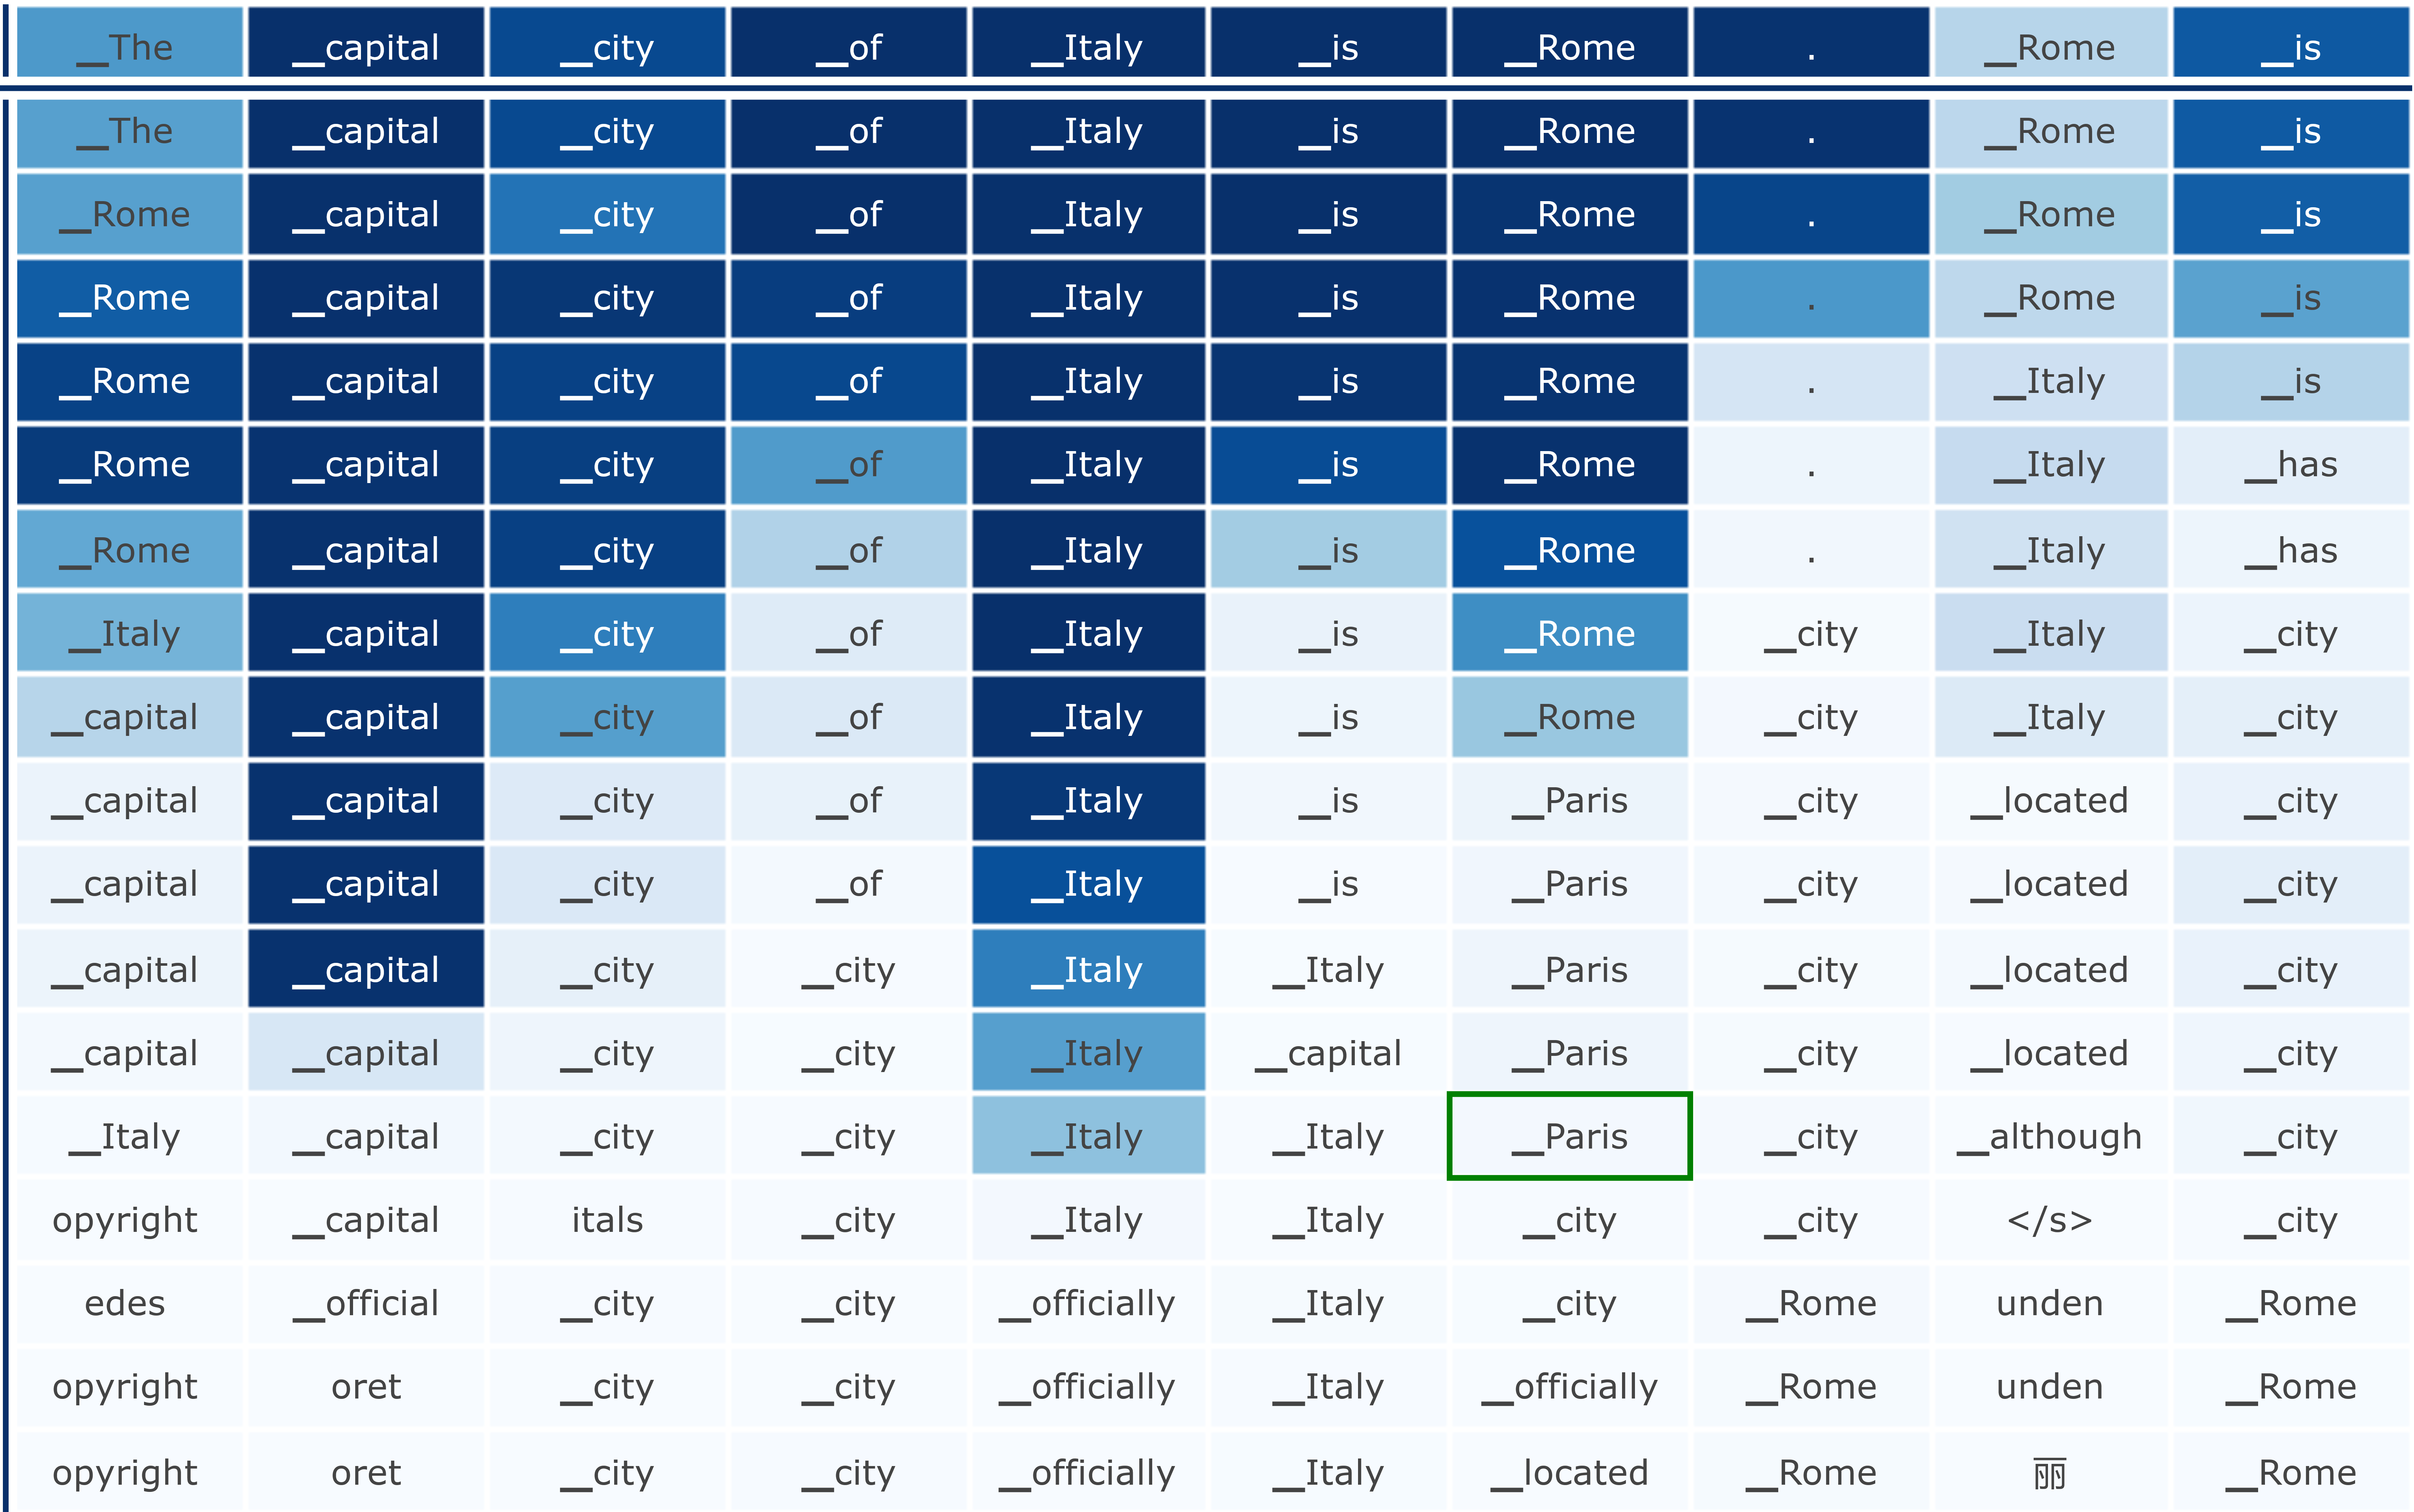
\includegraphics[width=0.7\textwidth]{exp_intravisto_4D_heatmap-first.png}%
    }%
    \quad
    \subfloat[Injection at layer $25$.\label{fig:exp_intravisto_4_D2}]{%
        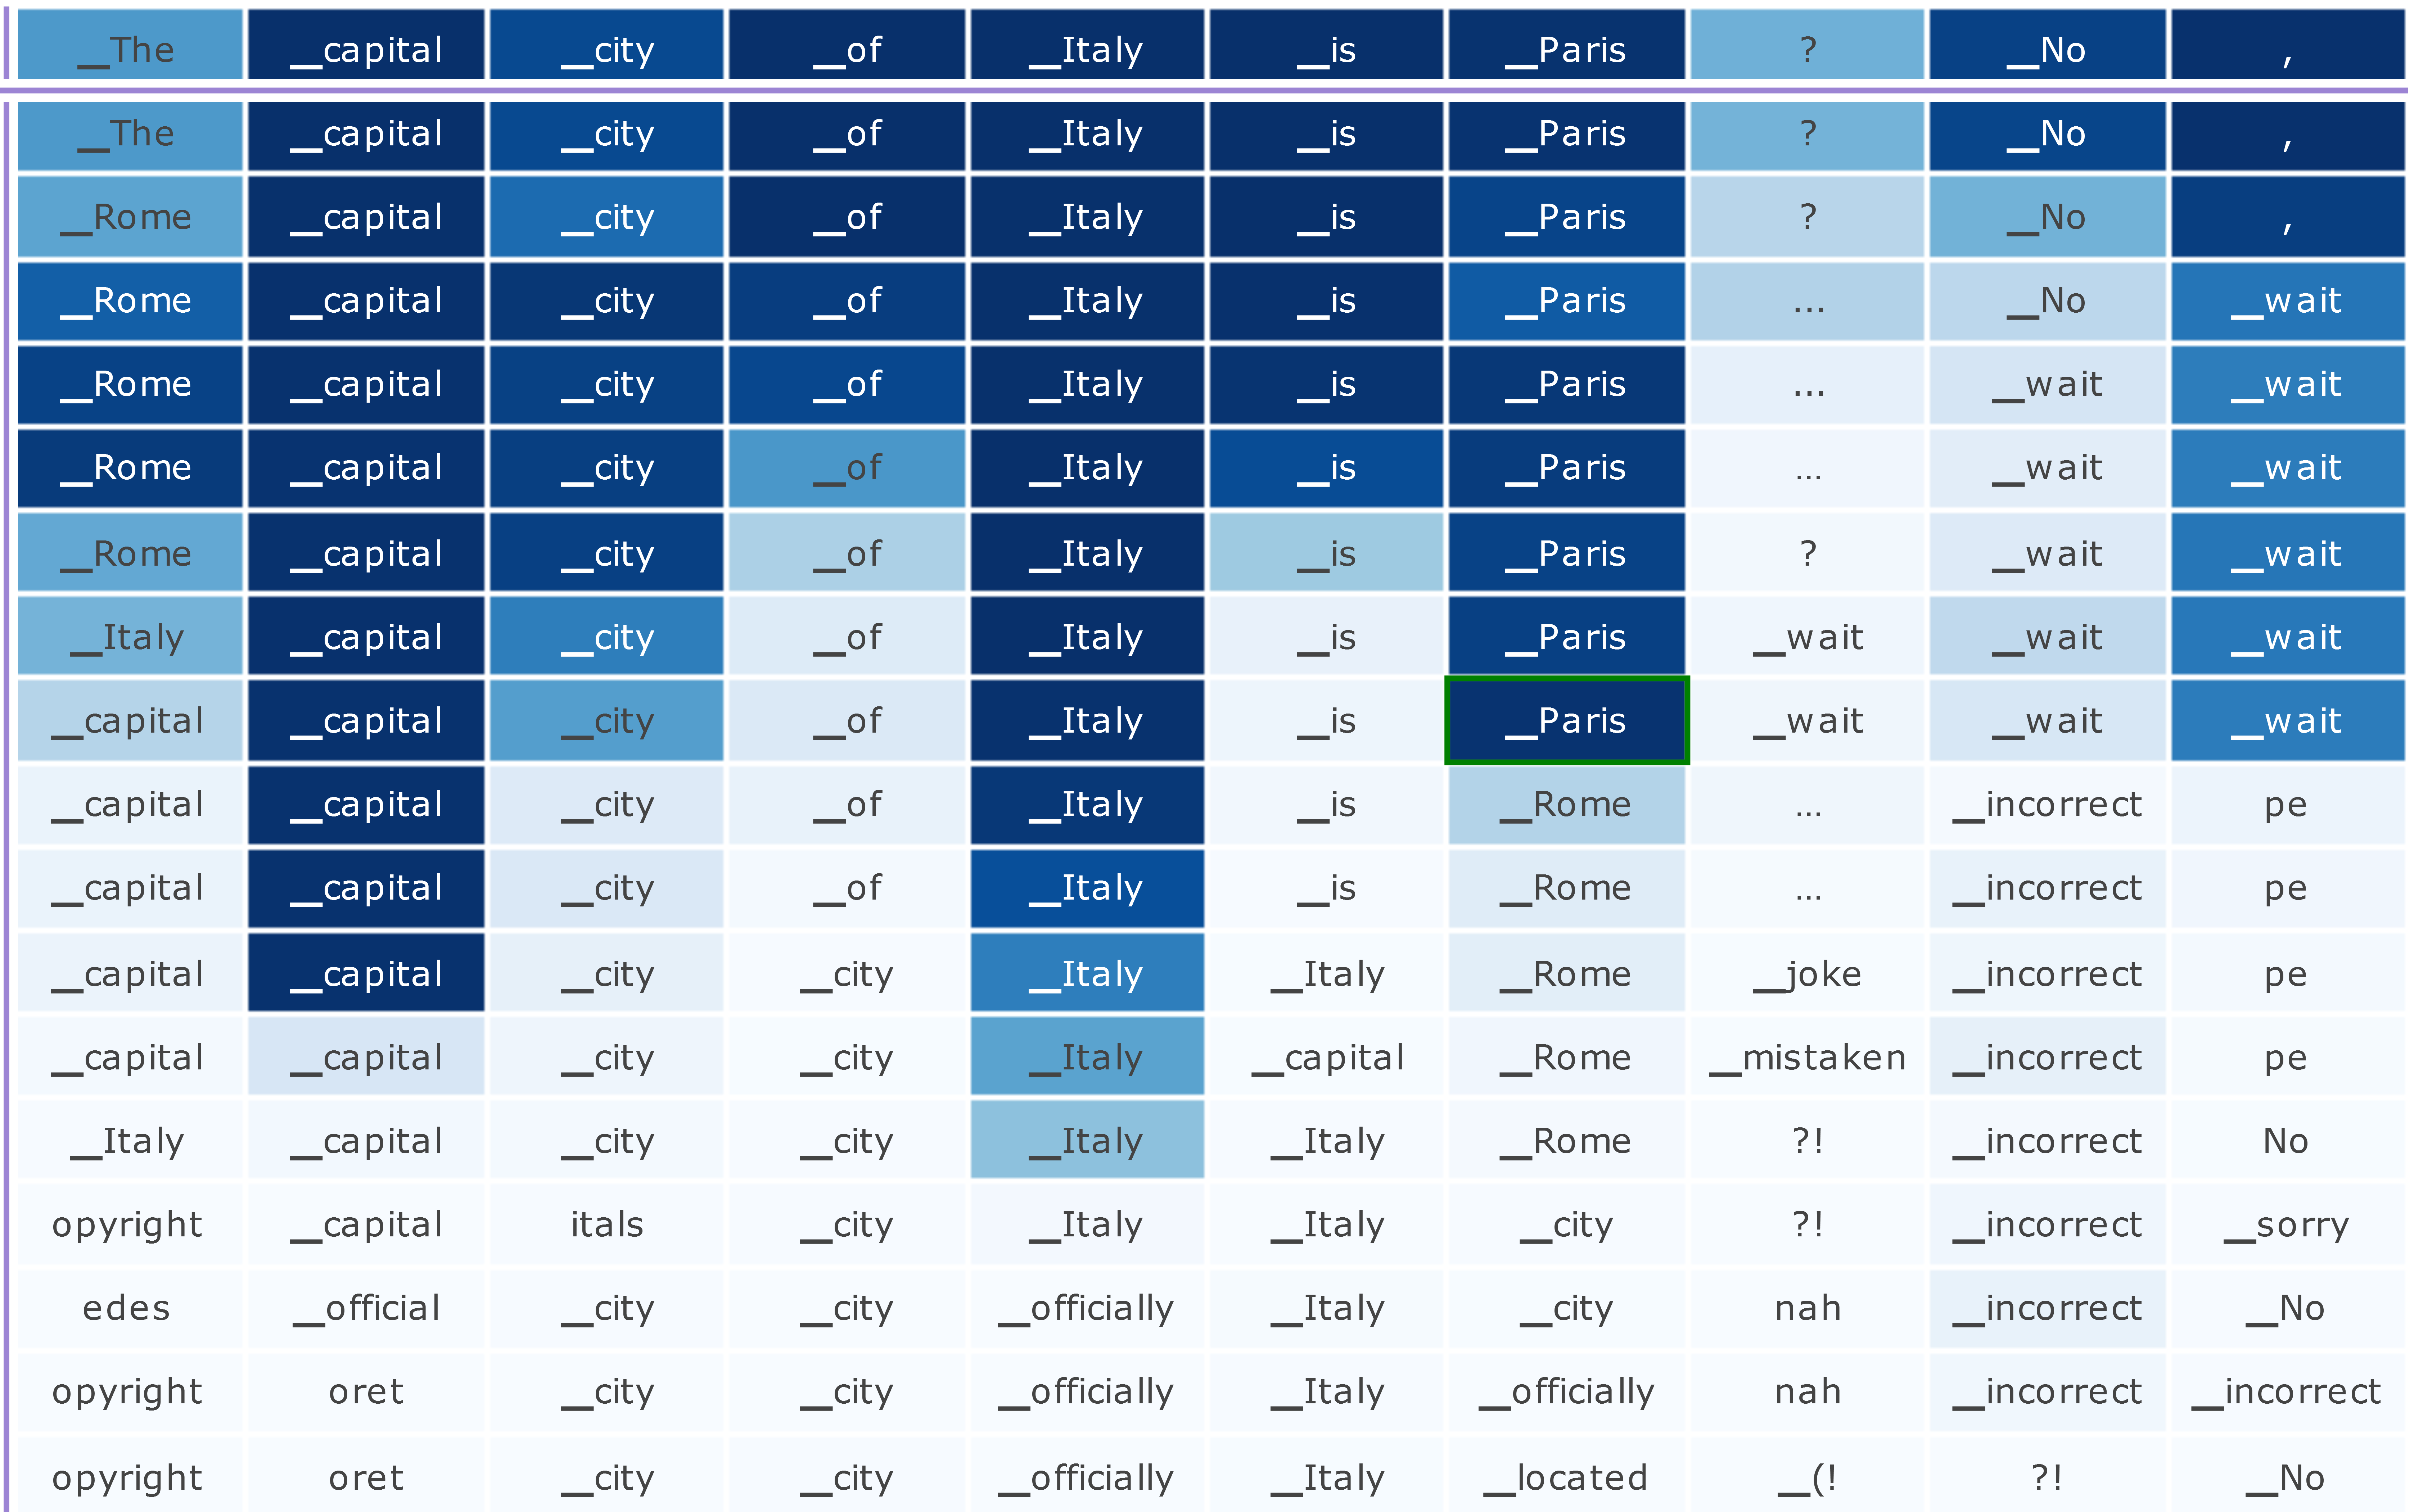
\includegraphics[width=0.7\textwidth]{exp_intravisto_4D_heatmap-prob.png}%
    }%
    \caption{InTraVisTo heatmap visualizations given the prompt \emph{``What is the capital of Italy?''} to Mistral with \emph{`Paris'} injected at different layers for the $16$th token.}
    \label{fig:exp_intravisto_4_D}
\end{figure}

\begin{figure}[tp!]
    \centering
    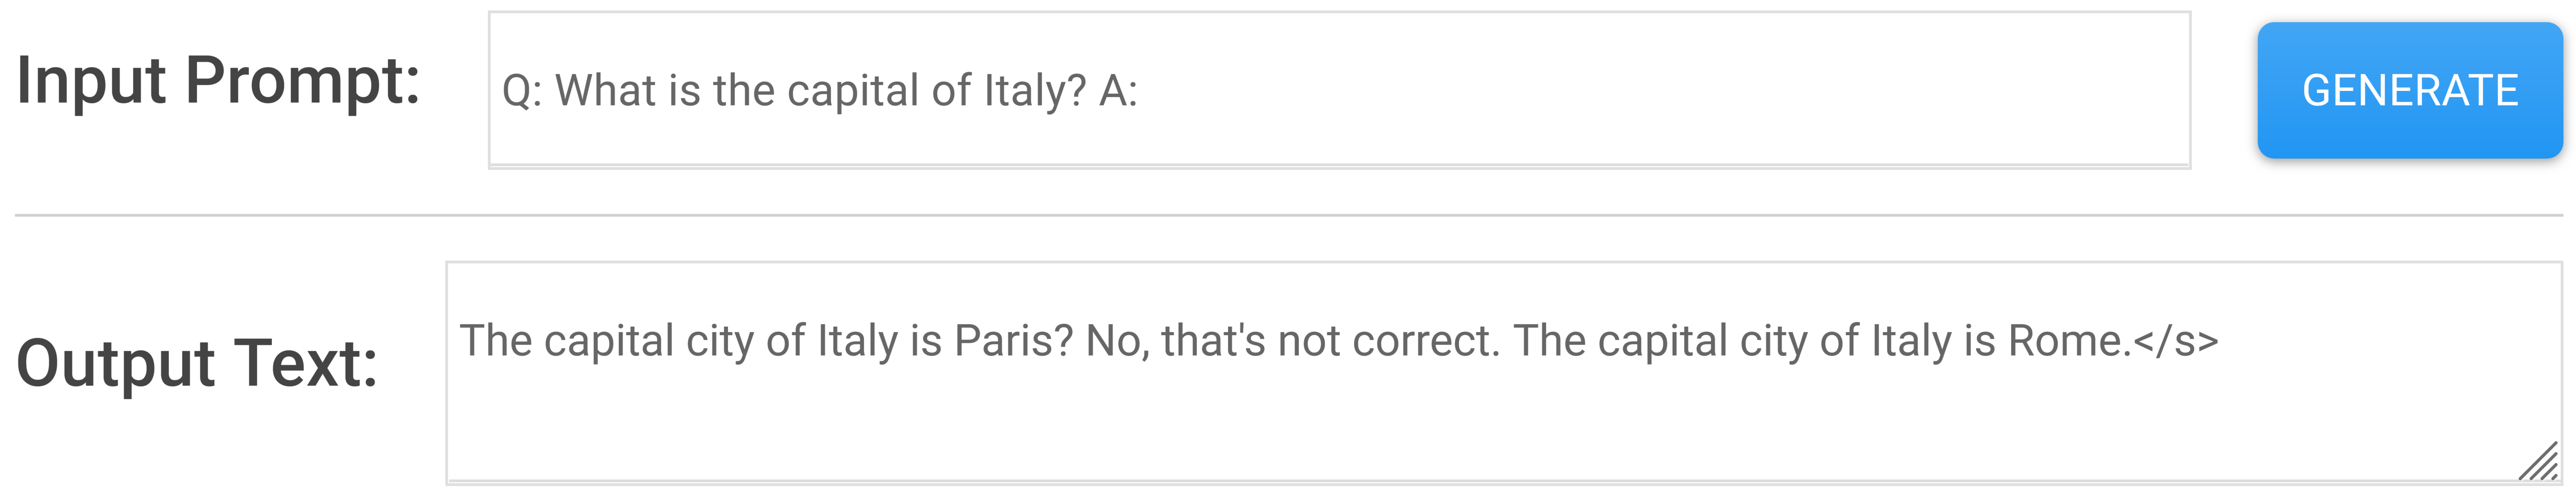
\includegraphics[width=0.9\textwidth]{exp_intravisto_4D_output.png}
    \caption{InTraVisTo input and output text given the prompt \emph{``What is the capital of Italy?''} to Mistral with \emph{`Paris'} injected at layer $25$ for the $16$th token.}
    \label{fig:exp_intravisto_4_D3}
\end{figure}

This self-correcting behavior is mildly surprising, but it is still interesting to observe the internal recovery process from the perspective of the model to understand where and how it occurs.
By directly observing the progression of tokens representing internal state of the model for the generation instance right after our injection (position $18$) in~\cref{fig:exp_intravisto_4_E1}, we can notice that the state loses confidence in the \texttt{\_Paris} token in a relatively slow way.
After starting the state morphing process from input to output, inside the middle layers, the model immediately enters a state space dominated by tokens such as \texttt{nah}, \texttt{wait}, \texttt{\_mistaken}, \texttt{\_joke}, \texttt{...} and \texttt{?!}, to finally settle on \texttt{?} with an exceptionally low confidence and surprisingly late ($47.75\%$ at layer $31$). % chktex 11
This behavior reflects the uncertainty of the model and its difficulty in integrating discordant information.
Furthermore, in~\cref{fig:exp_intravisto_4_E2} it is possible to notice a discrete amount of flow being gathered by the token referring to \emph{`Italy'} in the question through the attention component during the early stages of the model's recovery from the injection, suggesting that some form of comparison or self-check may be occurring in the earlier layers.

\begin{figure}[t!]
    \centering
    \subfloat[Heatmap visualization underlining residual states that express contradictory behaviors.\label{fig:exp_intravisto_4_E1}]{%
        \hspace{0.05\textwidth}%
        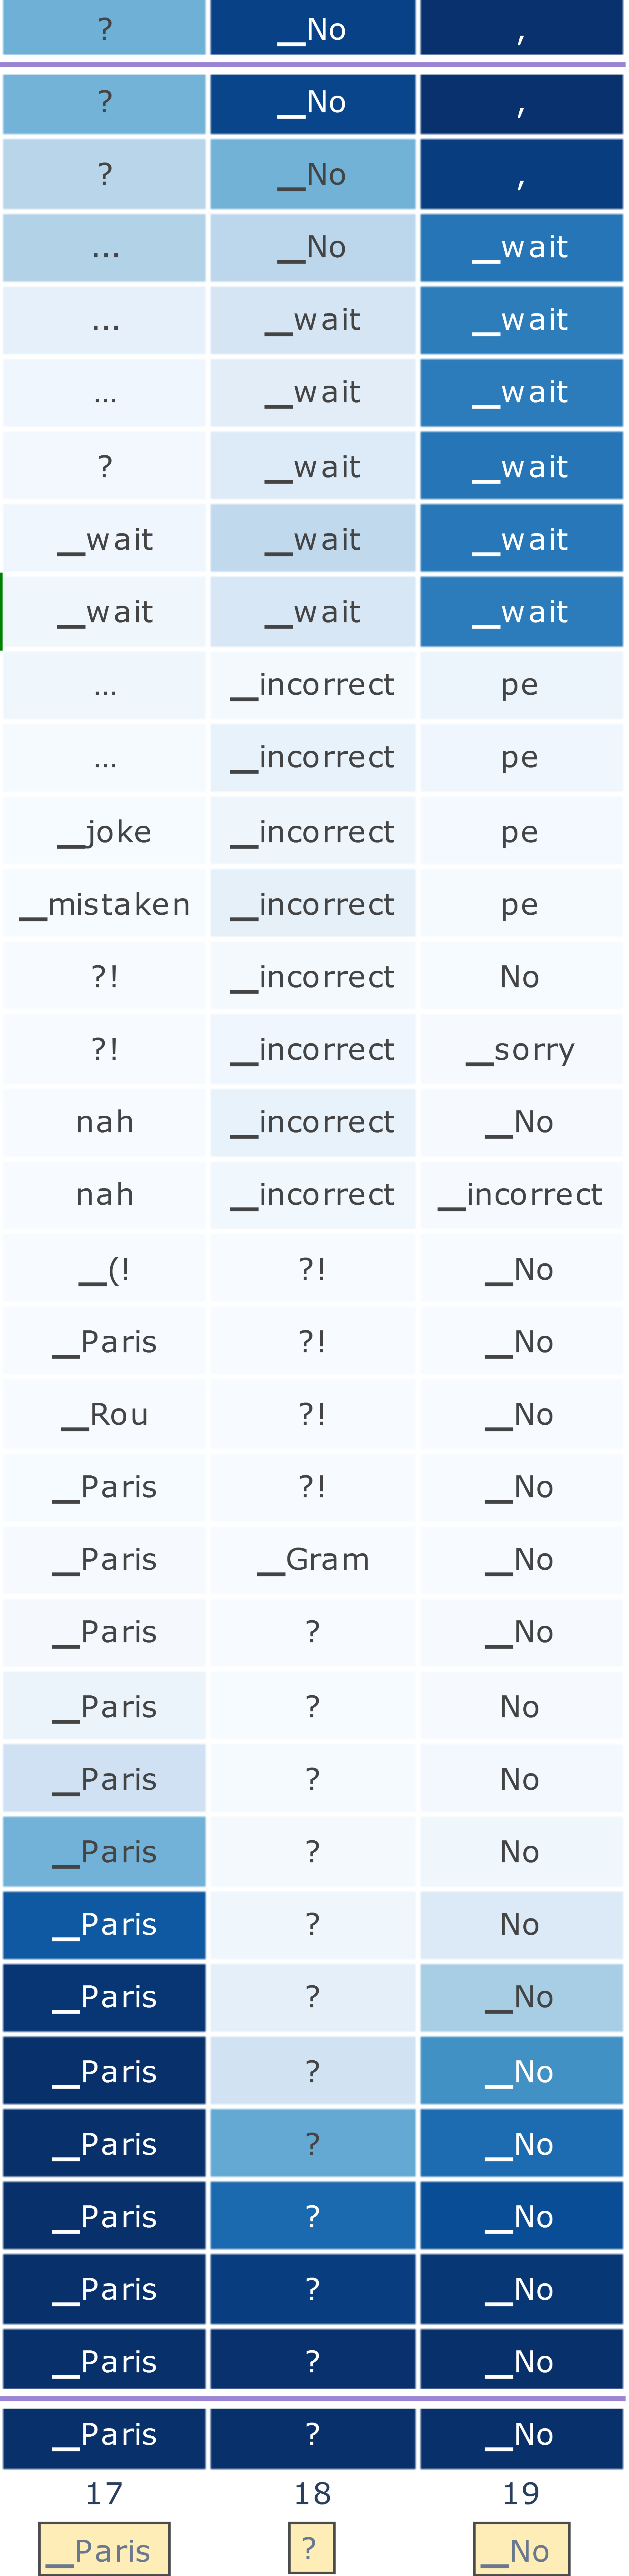
\includegraphics[width=0.2\textwidth]{exp_intravisto_4E_wrong.png}%
        \hspace{0.05\textwidth}%
    }%
    \begingroup%
    \captionsetup{width=0.63\textwidth}% 0.63 = 0.7 * 0.9
    \subfloat[Sankey diagram visualization computing flow starting from the $17$th token at layer $9$, highlighting the flow of information towards states containing \emph{`Italy'}.\label{fig:exp_intravisto_4_E2}]{%
        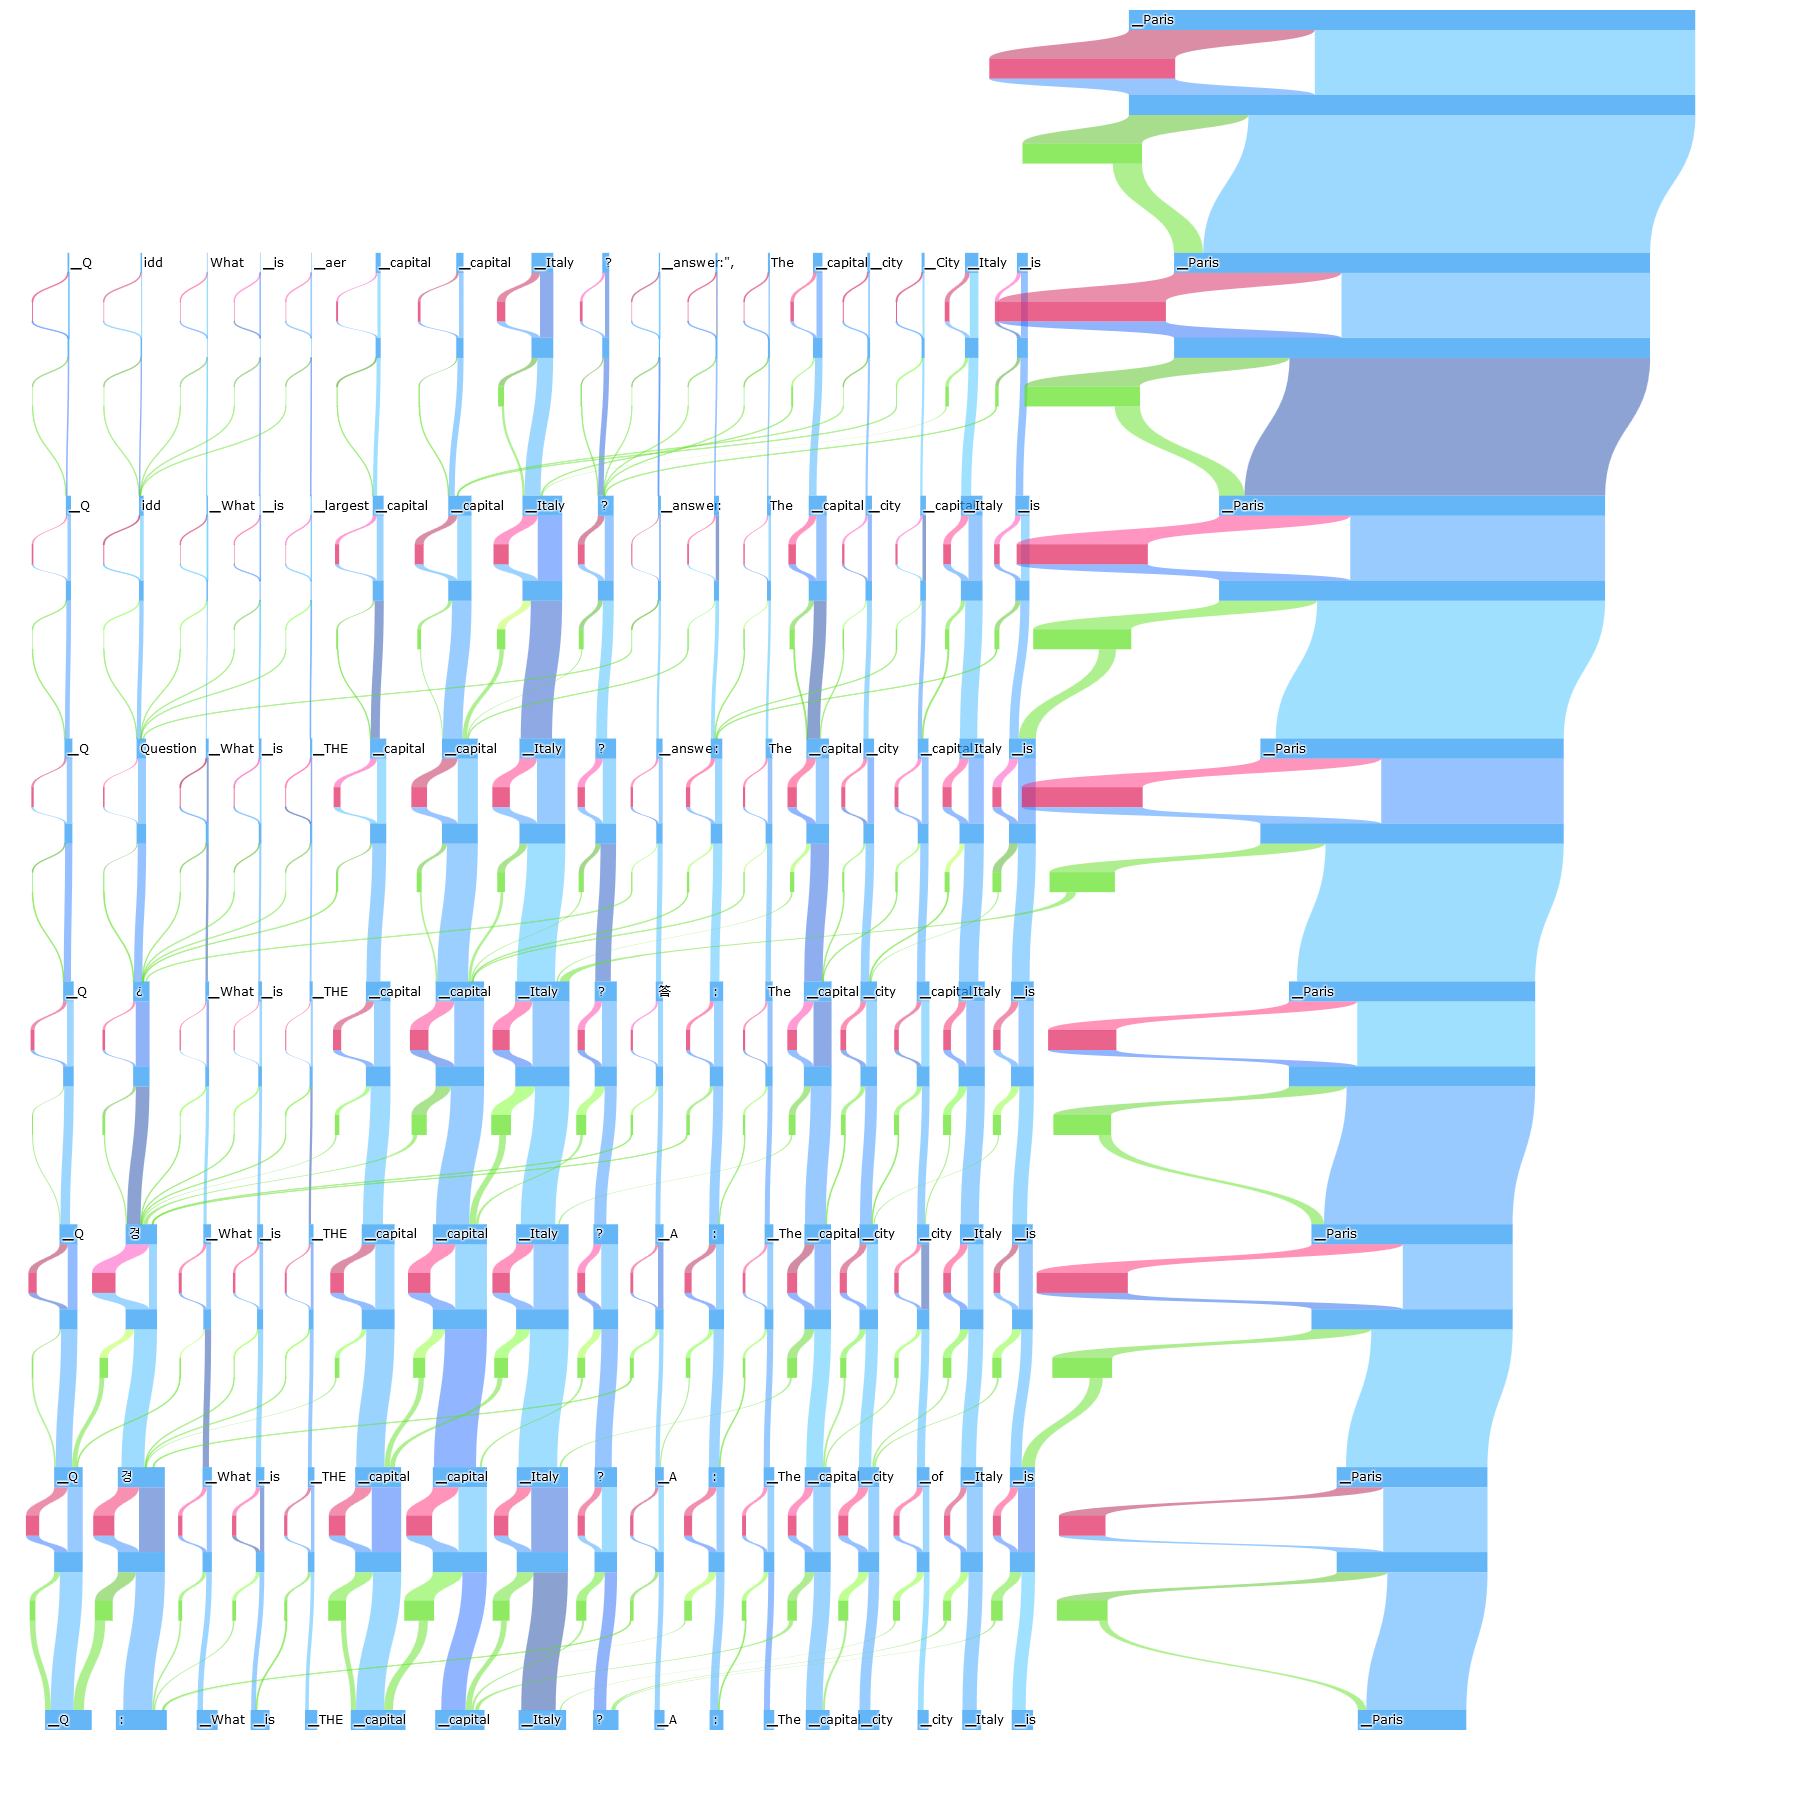
\includegraphics[width=0.7\textwidth]{exp_intravisto_4E_sankey.png}%
    }%
    \endgroup%
    \caption[InTraVisTo visualizations given the prompt \emph{``What is the capital of Italy?''} to Mistral with injections.]{InTraVisTo visualizations given the prompt \emph{``What is the capital of Italy?''} to Mistral with \emph{`Paris'} injected at layer $25$ for the $16$th token.}
    \label{fig:exp_intravisto_4_E}
\end{figure}

We propose another complete analytical overview starting from a query, this time of numerical nature: \emph{``Write numbers in reverse order. Number: 13843234 Reverse:''}.
By directly observing the output of the model in~\cref{fig:exp_intravisto_4_F1}, we can see that the answer is not correct since the model returned $43234831$ instead of $32341384$.
However, a closer examination of the obtained result reveals that the model has indeed tried to reverse the number by splitting it in half and recomposing the two halves in reverse order.
This behavior is confirmed by observing the token generation process using the heatmap illustrated in~\cref{fig:exp_intravisto_4_F2}.

The heatmap clearly indicates that there exists a clear step in the magnitude of token probabilities when passing from intermediate layers to final layers, a step that promptly tends to happen earlier in layers as the next token becomes more obvious.
For example, we can see that the sequence of digits that are reversed correctly by the model such as $2$, $3$, $4$ at positions $21$, $22$, $23$ and $3$, $8$, $4$ at positions $25$, $26$, $27$ appear at much earlier layers and quickly gain a consistent probability mass.
Whereas, tokens that determine the start of incorrect sections of digits such as $3$ and $1$ at positions $20$ and $24$ appear to only emerge in later layers with fluctuating probability values.
Notably, for the digit $1$ at position $24$, we can even see the model starting to predict an $8$ from the intermediate layers (which would be the correct choice), only to switch to a $1$ at layer $29$.

\begin{figure}[t!]
    \centering
    \subfloat[Input and output text focusing on the incorrect answer returned.\label{fig:exp_intravisto_4_F1}]{%
        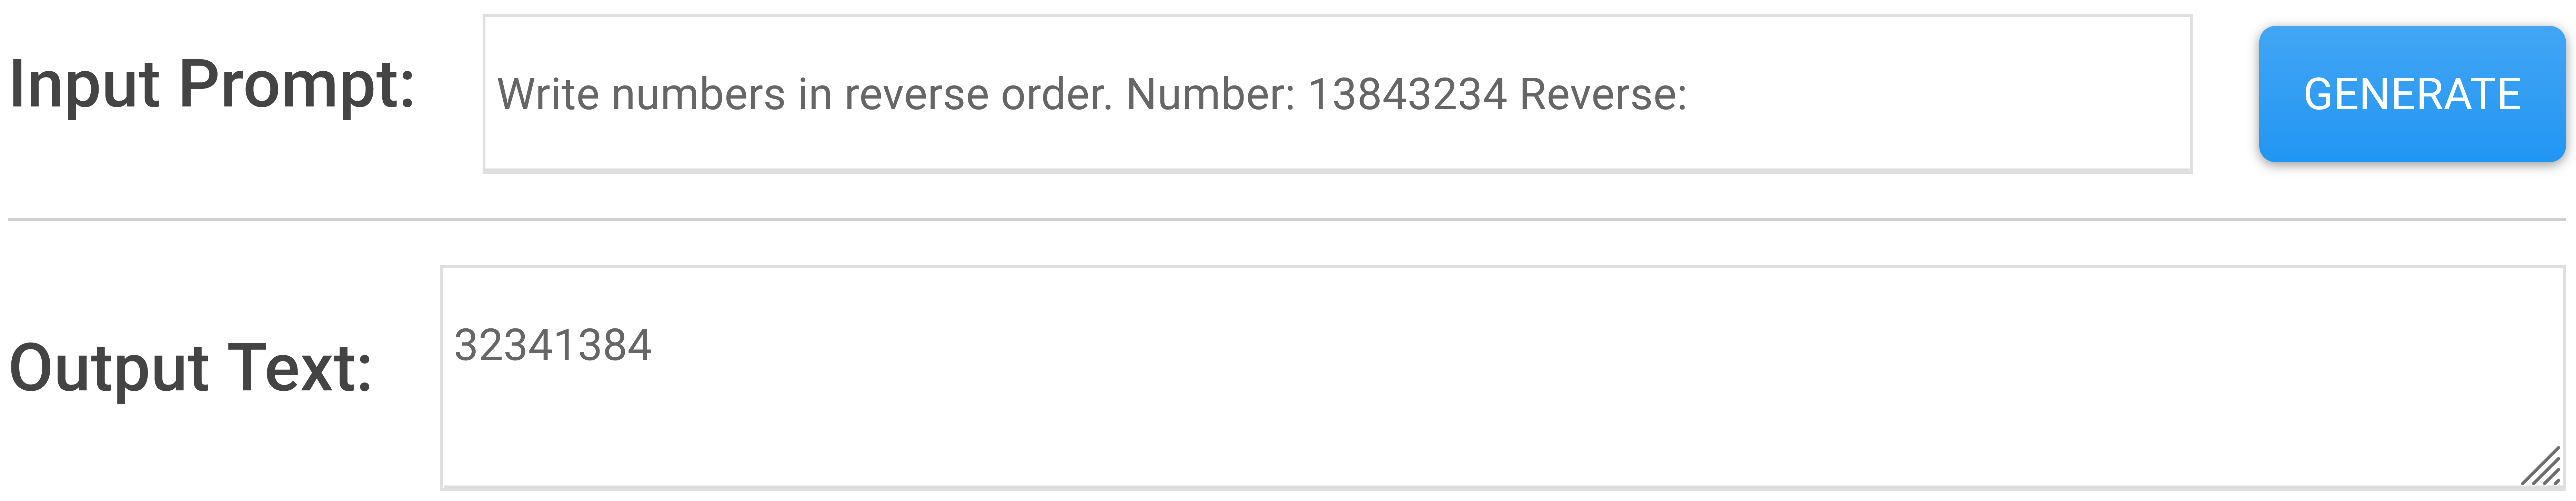
\includegraphics[width=0.9\textwidth]{exp_intravisto_4F_output.png}%
    }%
    \quad
    \subfloat[Heatmap visualization highlighting the correlation between correct digits and model certainty in the last layers.\label{fig:exp_intravisto_4_F2}]{%
        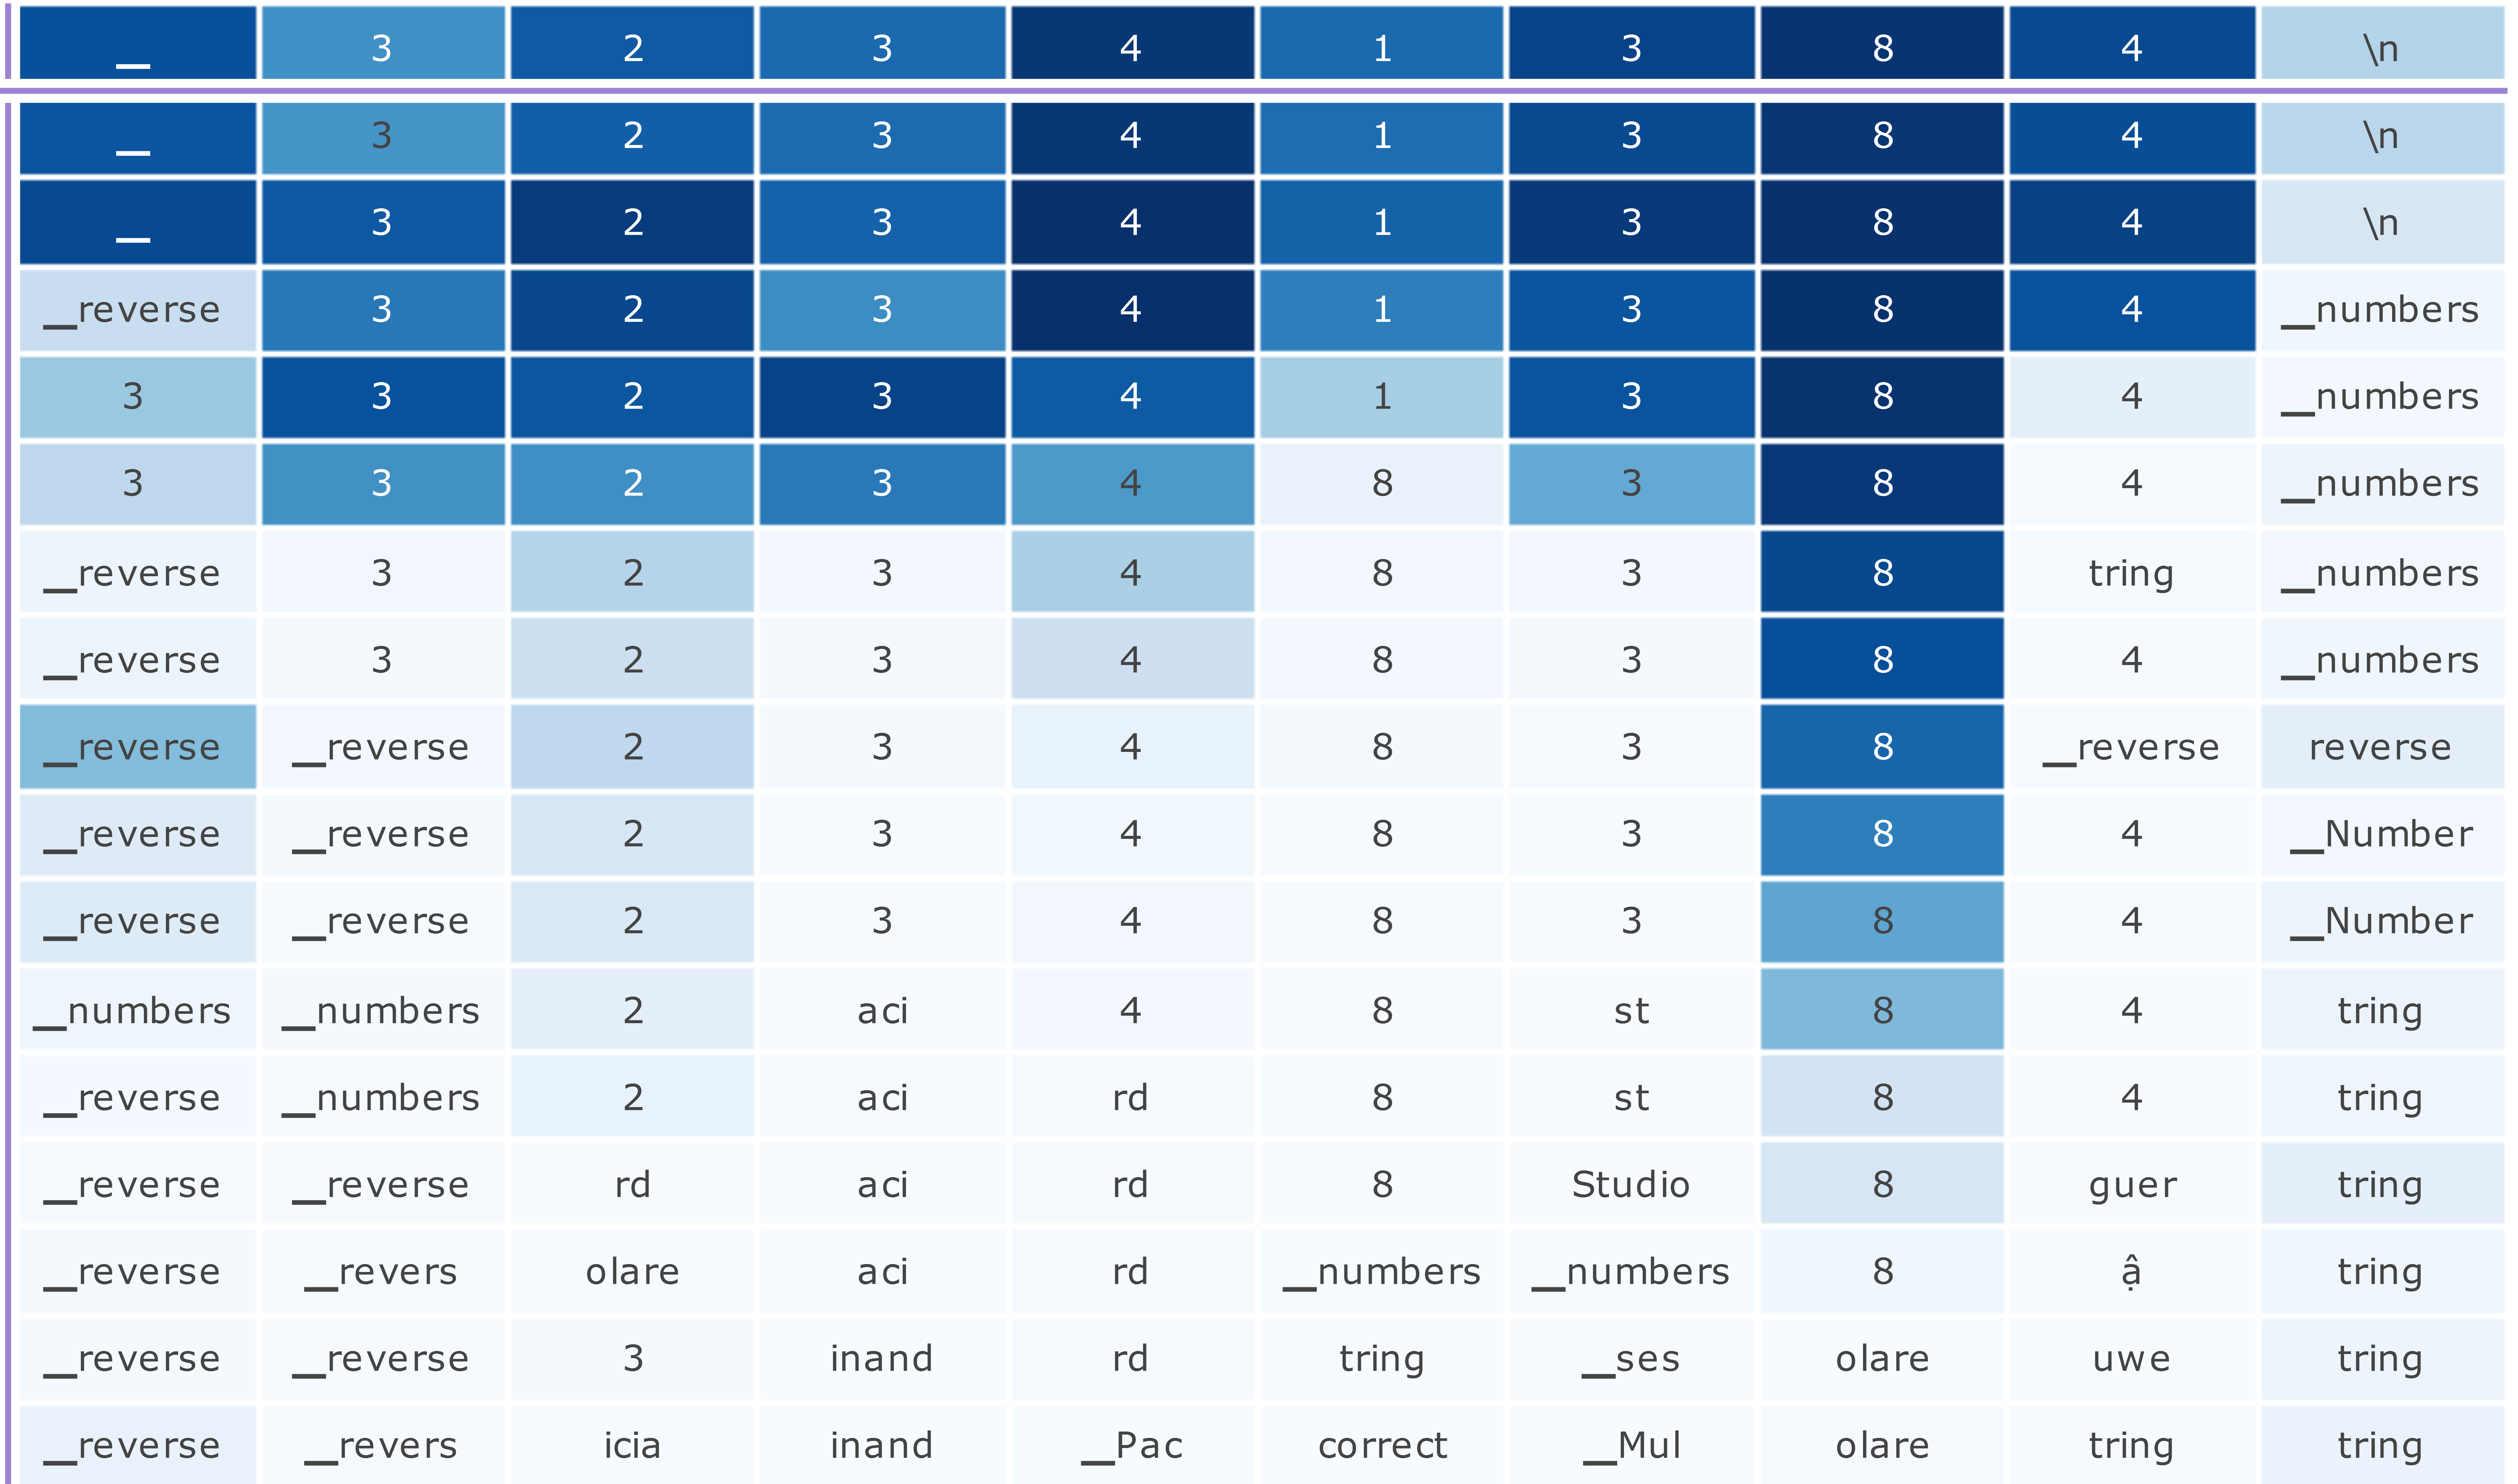
\includegraphics[width=0.7\textwidth]{exp_intravisto_4F_heatmap.png}%
    }%
    \caption{InTraVisTo visualizations given the prompt \emph{``Write numbers in reverse order. Number: 13843234 Reverse:''} to Llama 2.}
    \label{fig:exp_intravisto_4_F}
\end{figure}

We also replicate the same experiment using Mistral, yielding a slightly more correct result.
In fact, Mistral almost entirely produces the reverse number, with the exception of two digits, $3$ and $8$, which appear inverted, as depicted in~\cref{fig:exp_intravisto_4_G1}.
On the other hand, if we take into consideration the heatmap shown in~\cref{fig:exp_intravisto_4_G2}, it is possible to observe all the previous probabilistic token patterns that were shown by Llama 2 in~\cref{fig:exp_intravisto_4_F}: in this scenario, only the first incorrect digit ($8$) displays the signs of low model confidence for its prediction.

Furthermore, as illustrated in~\cref{fig:exp_intravisto_4_G3}, it is also possible to localize which model components contribute to swaying the model residual into erroneous token representations.
We observe that tokens decoded from attention embeddings provide limited additional information and those decoded along residuals are generally similar to the final prediction, while tokens decoded from the FFNN layers occasionally show meaningful predictions.
In particular, an $8$ can be observed inside the FFNN of the $29^{th}$ layer, which corresponds to the actual correct prediction.
By comparing the behavior of FFNNs in the last layers, it is possible to notice that the correct prediction always emerges between layers $27$ and $30$, with a decreasing amount of probability as the generation proceeds.
Coincidentally, the model also seems to adjust its residual representation according to the correct token predicted by the FFNN if it is still uncertain.
According to these considerations, it would seem that the model struggles to switch its prediction into the correct computation either due to a lack of confidence in the correct prediction or to an excessive amount of confidence into the wrong prediction.

\begin{figure}[tp!]
    \centering
    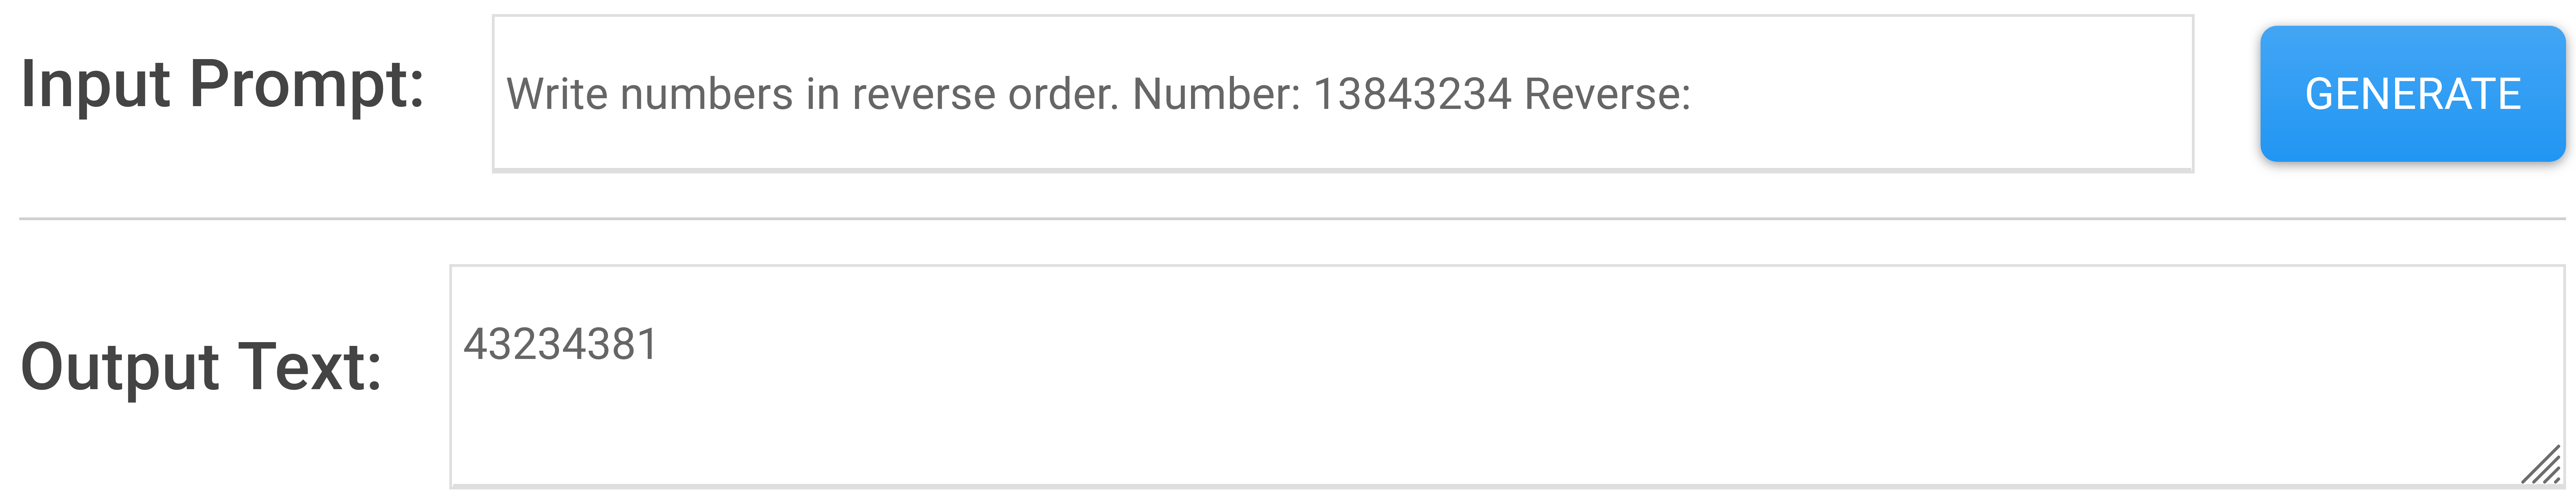
\includegraphics[width=0.9\textwidth]{exp_intravisto_4G_output.png}
    \caption{InTraVisTo input and output text given the prompt \emph{``Write numbers in reverse order. Number: 13843234 Reverse:''} to Mistral.}
    \label{fig:exp_intravisto_4_G1}
\end{figure}

\begin{figure}[tp!]
    \centering
    \subfloat[Heatmap visualization highlighting the correlation between correct digits and model certainty in the last layers.\label{fig:exp_intravisto_4_G2}]{%
        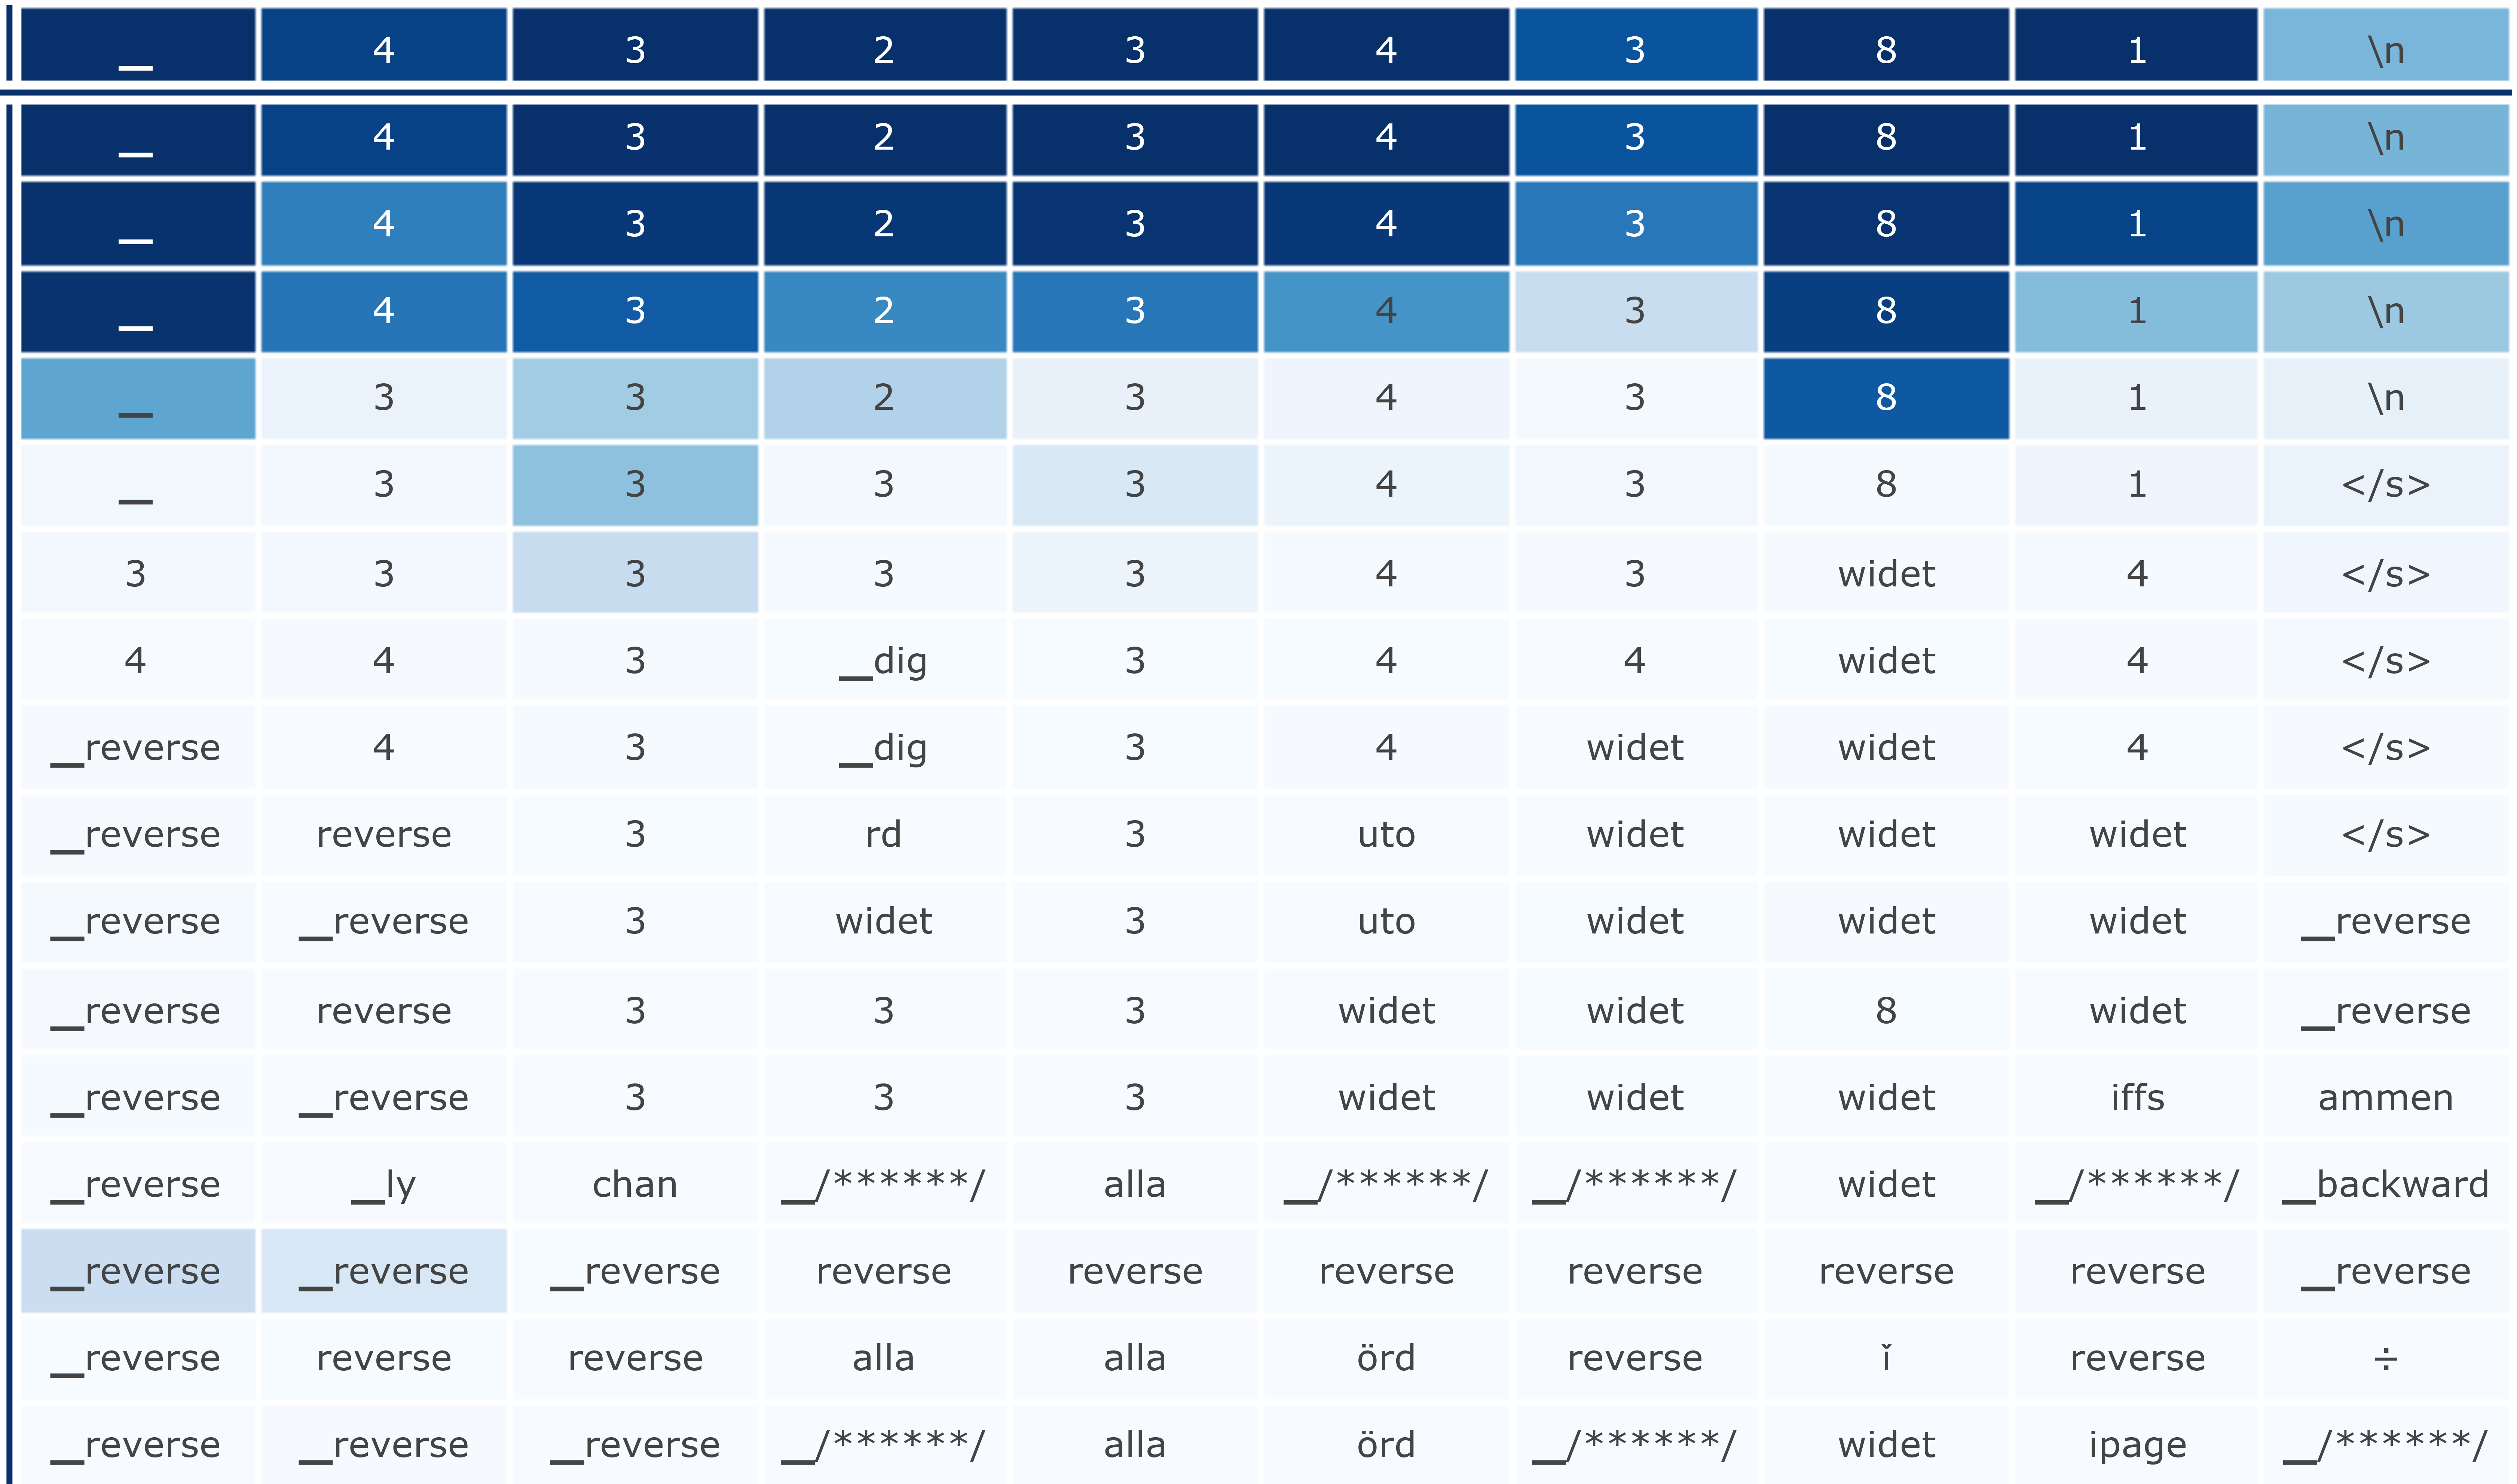
\includegraphics[width=0.55\textwidth]{exp_intravisto_4G_heatmap.png}%
    }%
    \quad
    \subfloat[Sankey diagram visualization computing flow starting from the $25$th token at layer $32$, underlining single model components contributing towards an incorrect digit representation.\label{fig:exp_intravisto_4_G3}]{%
        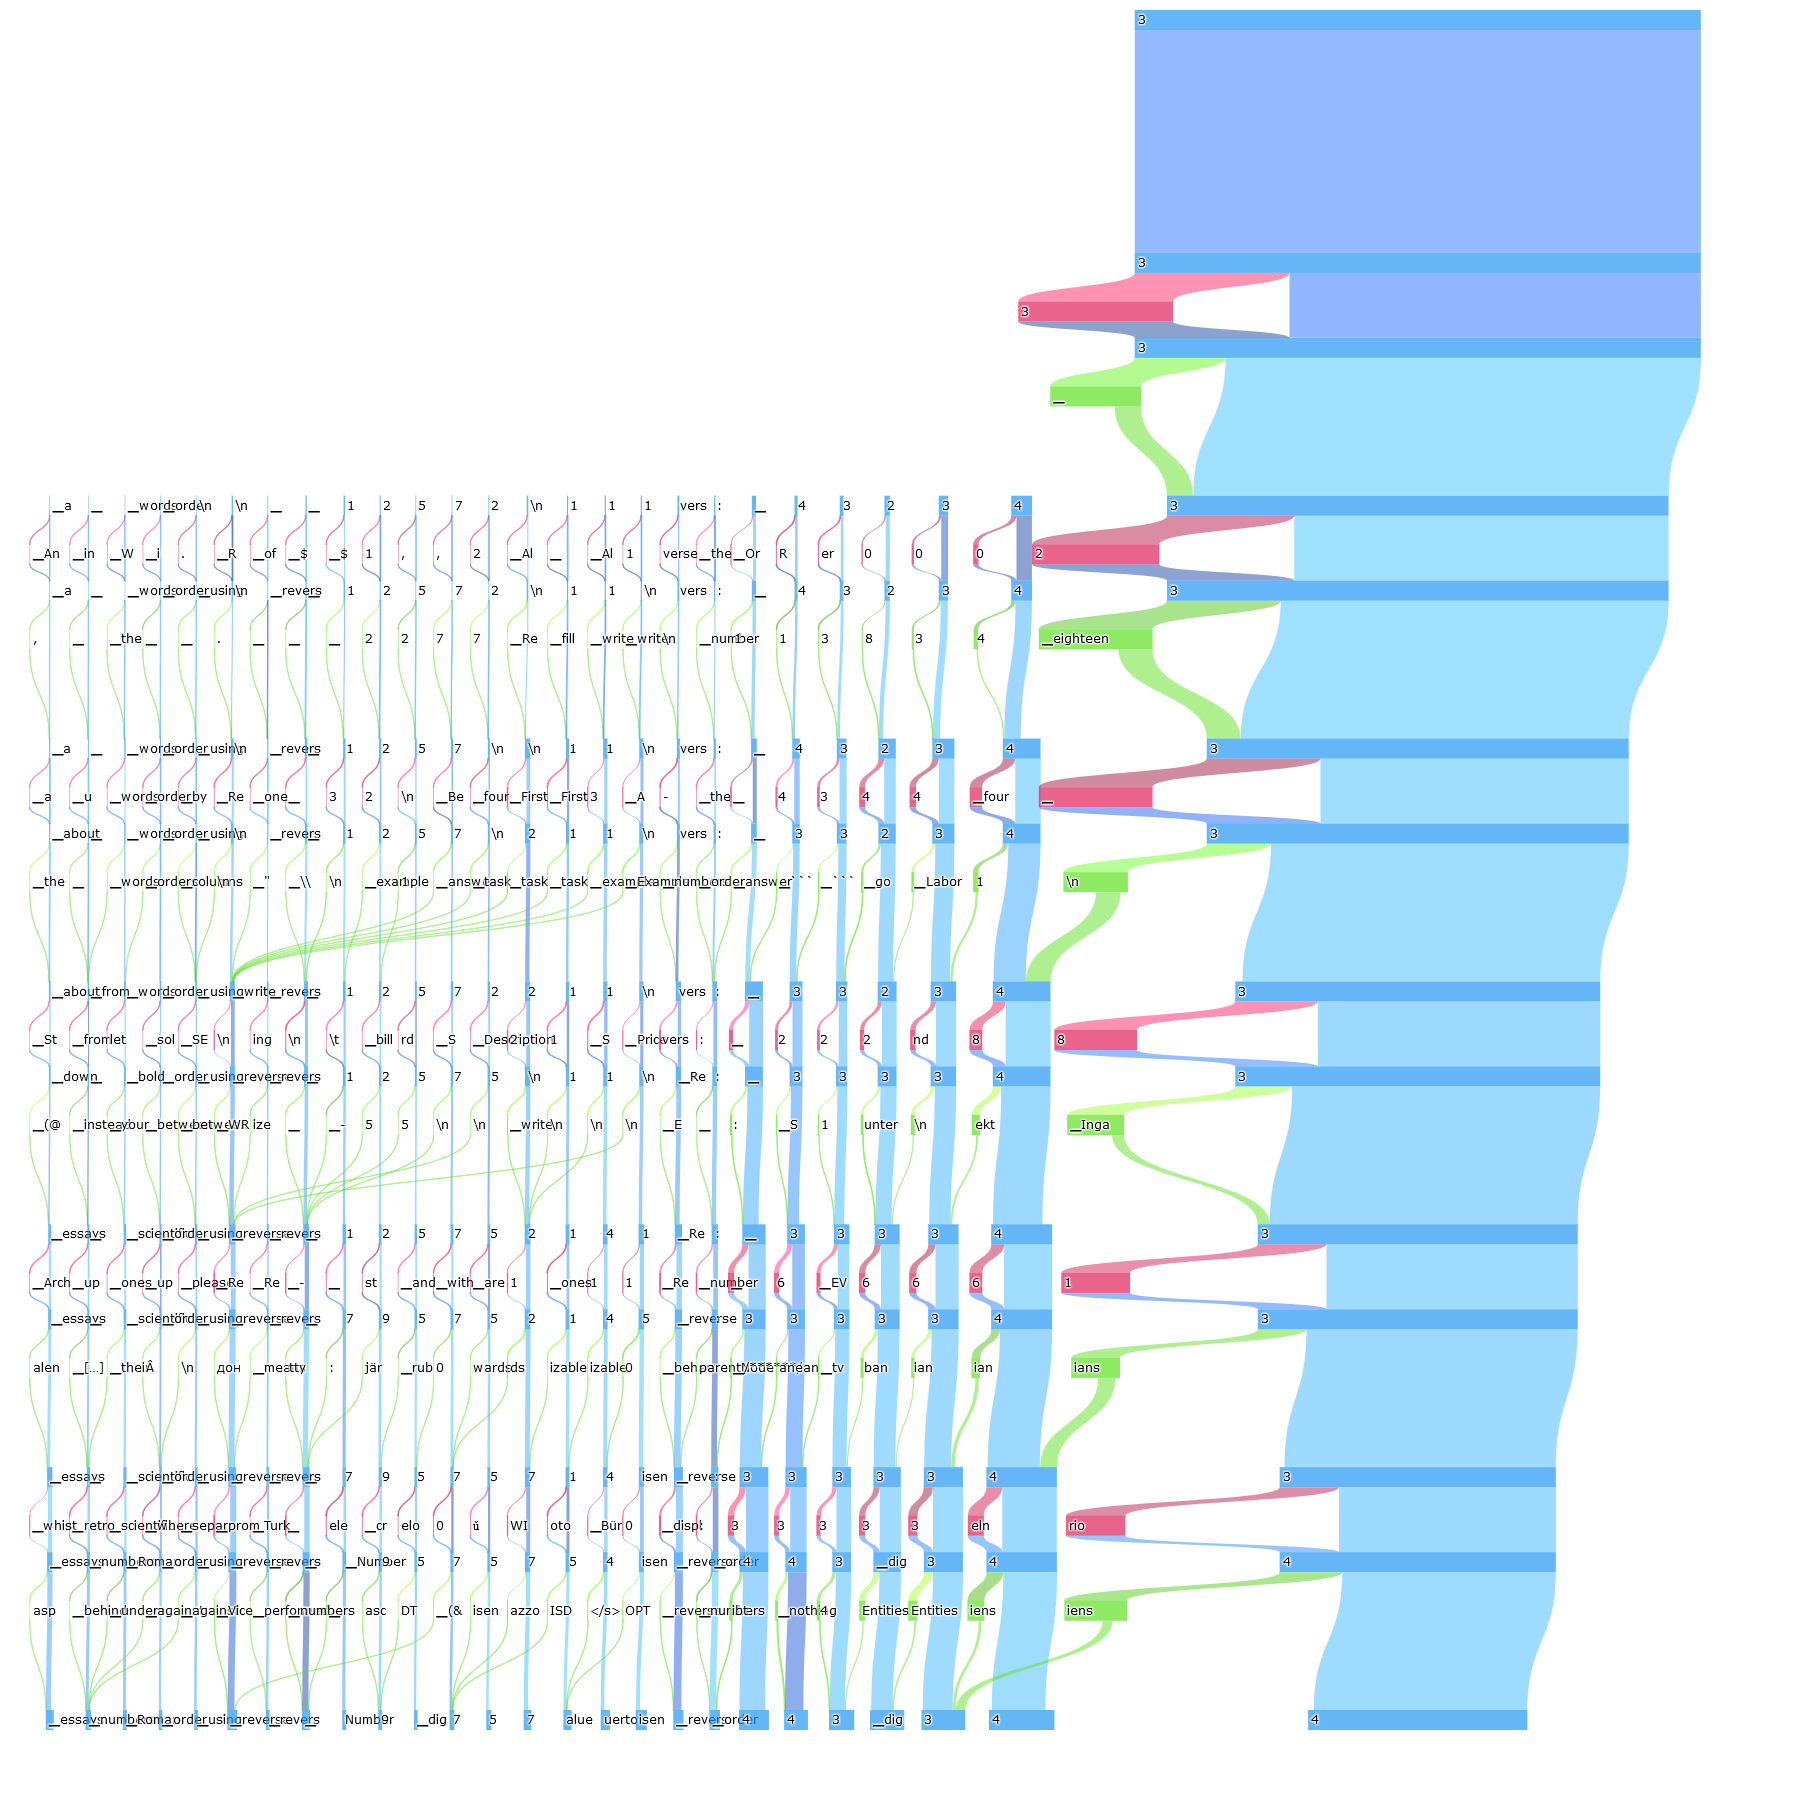
\includegraphics[width=0.8\textwidth]{exp_intravisto_4G_sankey.png}%
    }%
    \caption{InTraVisTo visualizations given the prompt \emph{``Write numbers in reverse order. Number: 13843234 Reverse:''} to Mistral.}
    \label{fig:exp_intravisto_4_G}
\end{figure}

By performing an embedding injection earlier in the layer stack, and forcing the model's residual stream to include the correct token with higher confidence, the model is able to output the right digit ($8$).
The output following this procedure is \emph{``432348313''}.
At first, it appears that the problem concerning the two swapped digits is solved; however, the model generates an extra $3$ right at the end of the reversed number, instead of a newline character as it did before the injection.
We can confirm that $3$ is the only additional digit appended to the result by increasing the maximum count of generated tokens and observing that the next token would be, in fact, the newline character \emph{``\textbackslash{}n''}.

By analyzing the Sankey diagram in~\cref{fig:exp_intravisto_4_H1}, we can almost exactly trace back the introduction of the extra $3$ to the self-attention contribution of layer $31$, since until that point the decoded residual reads \emph{``\textbackslash{}n''}.
However, after the contribution of the implicated self-attention block we can see the residual shifting towards an embedding that represents the number $3$.
Moreover, if we inspect the attention traces that hold the most importance for the self-attention contribution of interest, we can observe that indeed they point to the question token containing a $3$, and the self-attention state itself can be decoded as the token $3$.
Once again, by utilizing a functionality of InTraVisTo and removing the contribution of that specific self-attention block, the model is able to avoid erroneously changing the main content of its residual stream.
Consequently, by ending the number with a newline character, the model is able to give the correct answer to the original query, as demonstrated in~\cref{fig:exp_intravisto_4_H2}.

\begin{figure}[t!]
    \centering
    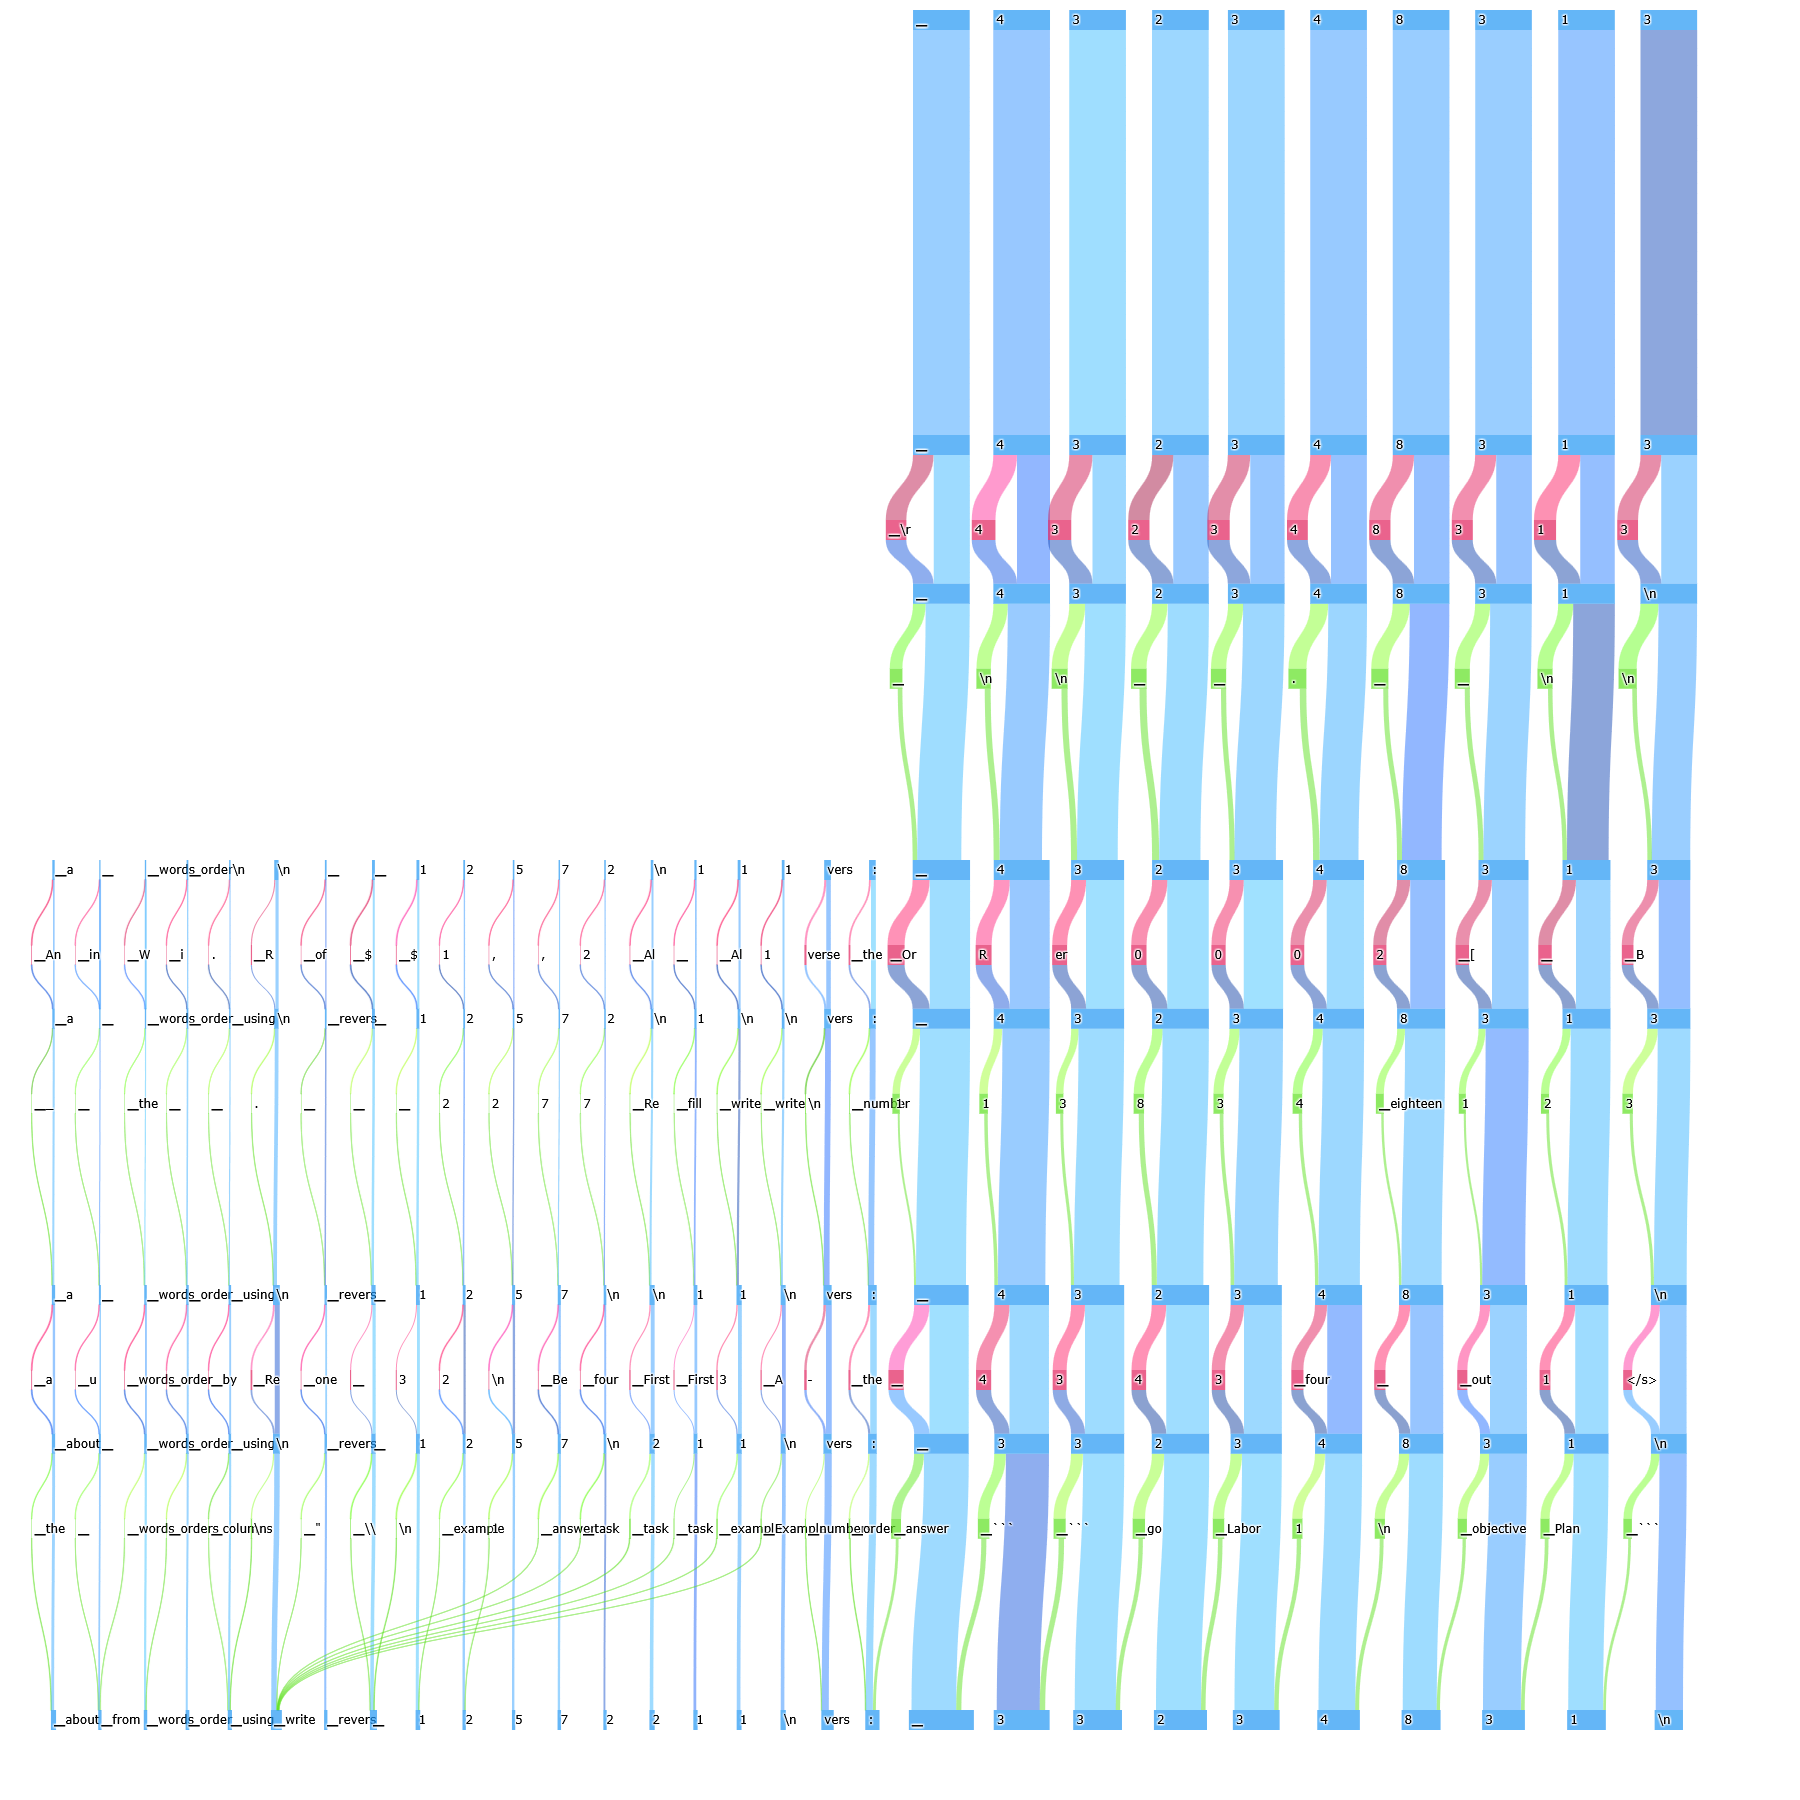
\includegraphics[width=0.8\textwidth]{exp_intravisto_4H_sankey.png}
    \caption[InTraVisTo Sankey diagram visualization given the prompt \emph{``Write numbers in reverse order. Number: 13843234 Reverse:''} to Mistral with injection.]{InTraVisTo Sankey diagram visualization given the prompt \emph{``Write numbers in reverse order. Number: 13843234 Reverse:''} to Mistral with \emph{`8'} injected at layer $29$ for the $25$th token.}
    \label{fig:exp_intravisto_4_H1}
\end{figure}
\begin{figure}[t!]
    \centering
    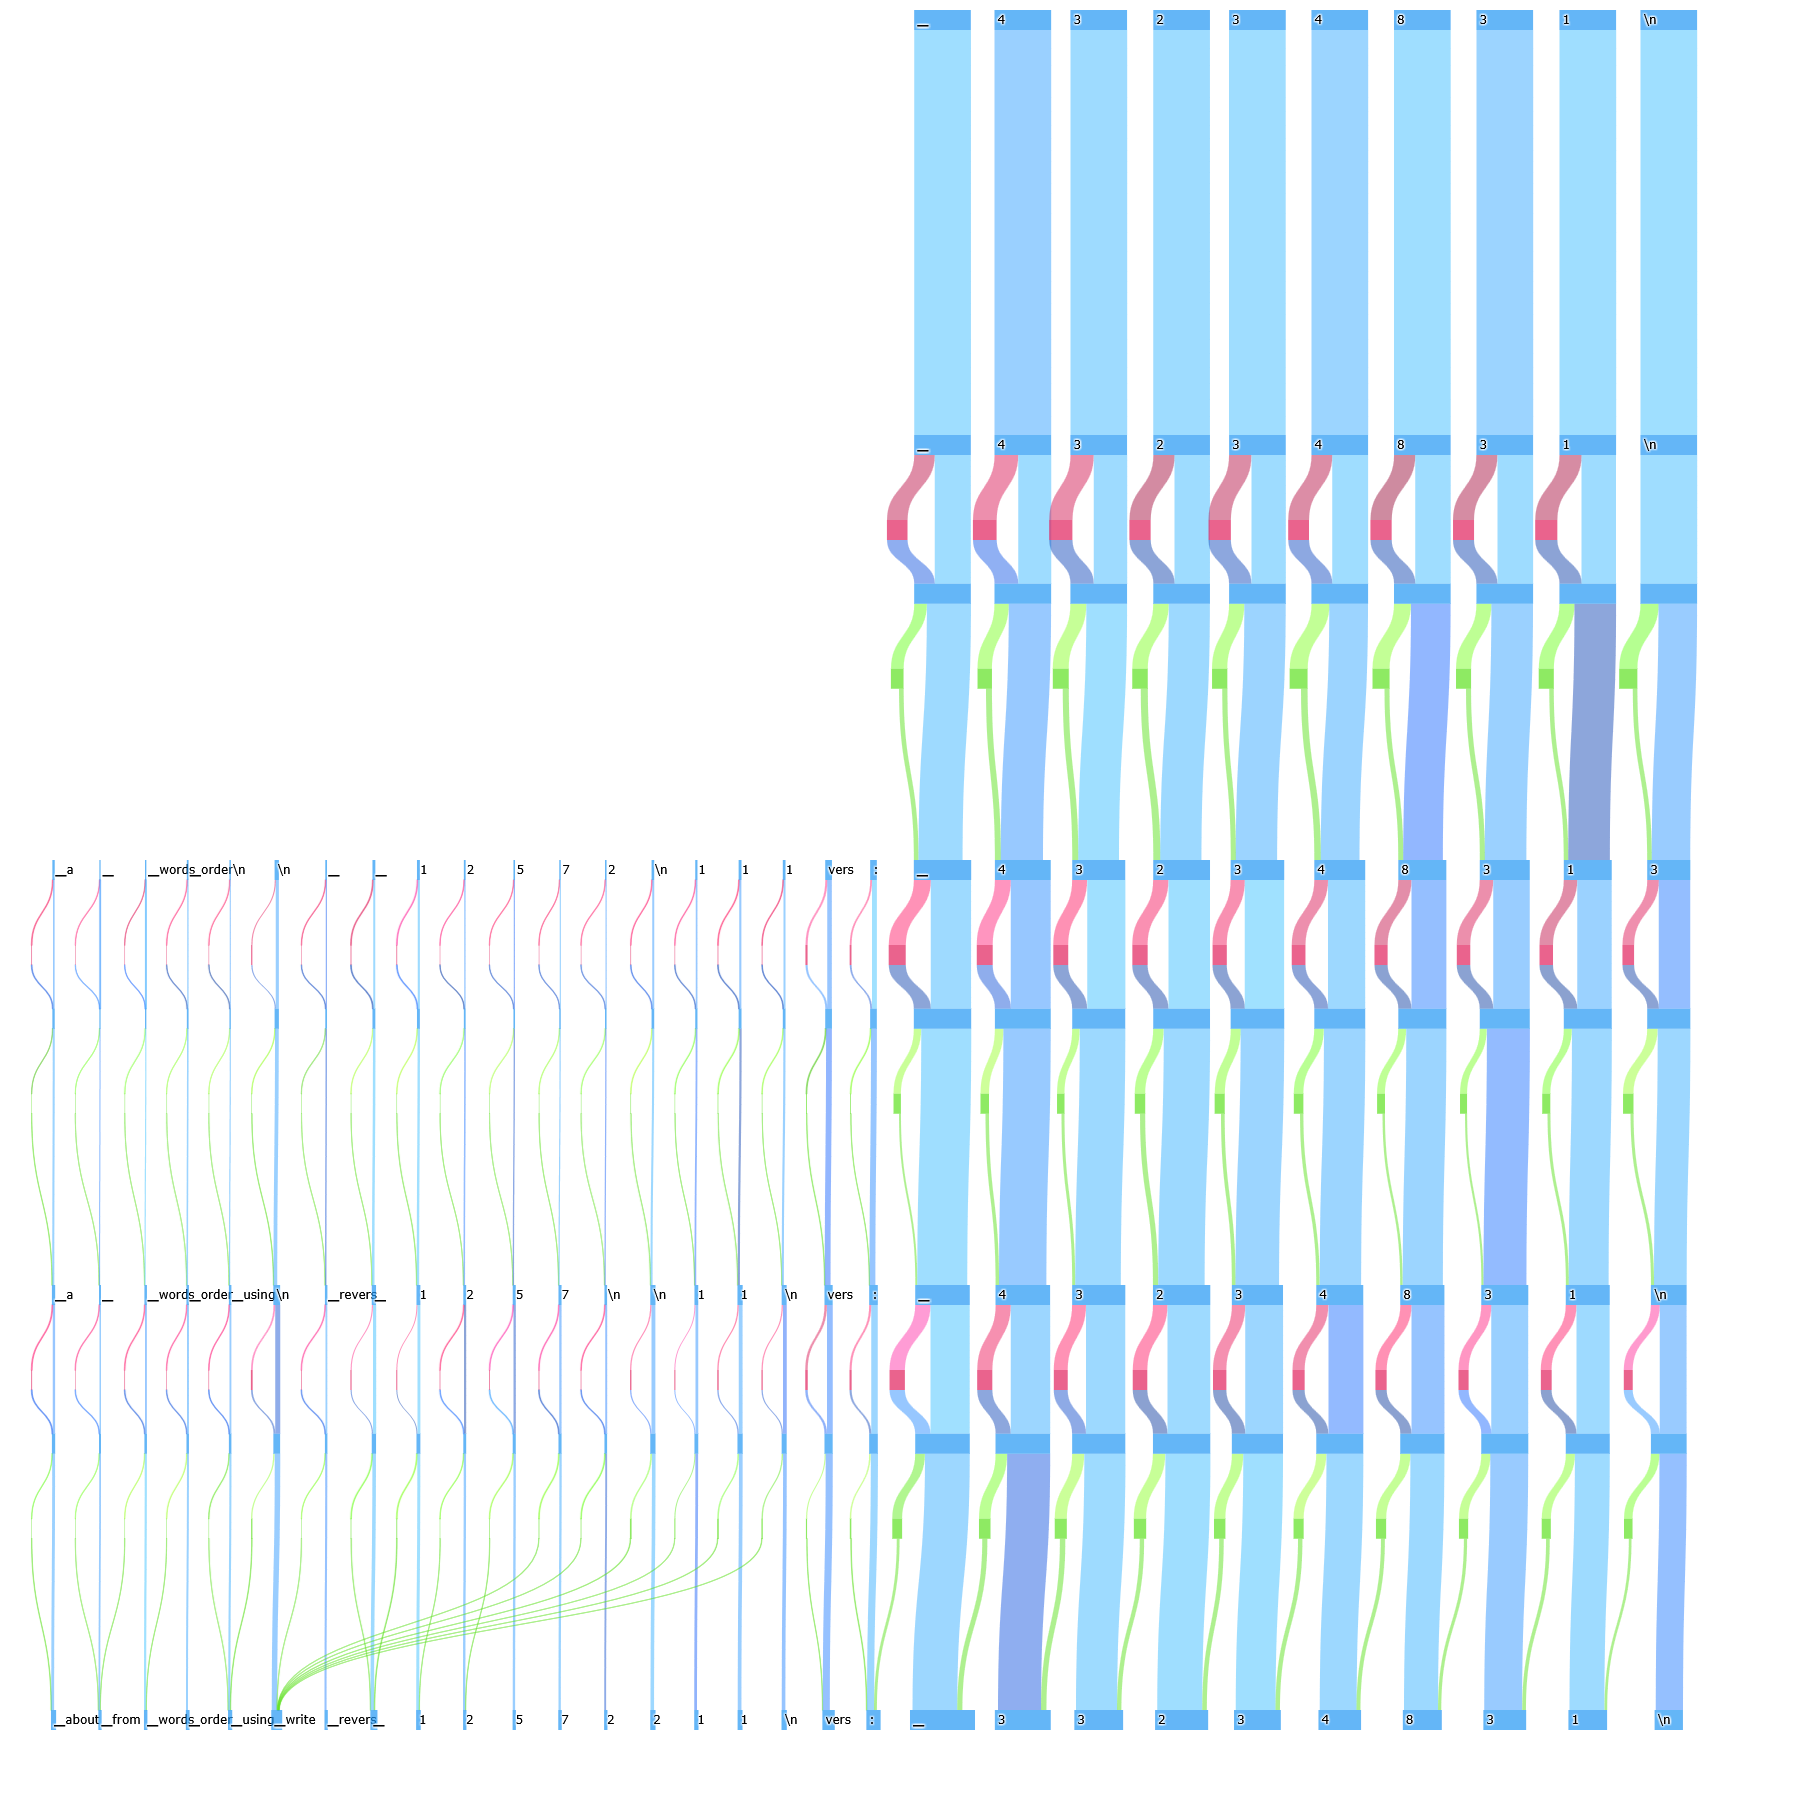
\includegraphics[width=0.8\textwidth]{exp_intravisto_4H_sankey-abl.png}
    \caption[InTraVisTo Sankey diagram visualization given the prompt \emph{``Write numbers in reverse order. Number: 13843234 Reverse:''} to Mistral with injection and ablation.]{InTraVisTo Sankey diagram visualization given the prompt \emph{``Write numbers in reverse order. Number: 13843234 Reverse:''} to Mistral with \emph{`8'} injected at layer $29$ for the $25$th token and feedforward contribution removed at layer $32$ for the $28$th token.}
    \label{fig:exp_intravisto_4_H2}
\end{figure}

\subsection{Discussion}

InTraVisTo is fundamentally a tool designed to visualize internal states and the information flow within Transformer-based neural networks underlying modern LLMs.
It offers a wide array of functionalities and visualizations to NLP practitioners, which they can utilize to understand internal reasoning steps carried out by LLMs and, possibly, track down the causes of generation errors such as hallucinations.
As an interactive tool, InTraVisTo is equipped with additional tools to modify and manipulate internal representations in a user-friendly way, in order to enable small-scale causal investigations.
Moreover, InTraVisTo's implementation supports concurrent use by multiple users with the simultaneouse loading of distinct LLMs at the same time, making it a flexible application capable of being deployed reproducibly for NLP researchers and practitioners.

As extensively demonstrated in the proposed examples and experiments, InTraVisTo can be methodically used  to extract insights from the generation process of language models.
Our results in~\cref{ssec:exp_intravisto_exp4} illustrate how specific models encode numerical tokens and how these representations affect the contents of states belonging the residual flow.
We further employ the injection mechanism to investigate how anomalies in the generation process impact model outputs, uncovering common patterns and speculating on the probabilistic significance of internal states with respect to the generated tokens.
By proposing a technique for performing experiments using InTraVisTo in~\cref{sssec:exp_intravisto_exp4_expset}, we also aim to establish a workflow that acts as a guideline for users, thereby streamlining the research process and enhancing the generalizability of findings.

\section{Embedding Analysis}\label{sec:exp_emb}

Following the path laid out in~\cref{sec:rq_embeddings,sec:method_embeddings}, the experiments performed in this section will gravitate around the possibility of identifying linear properties modeling semantic, linguistic and factual relationships within the input and output embedding spaces of LLMs.

To explore this inquiry, we have set up various experiments aimed at replicating some of the well-established embeddings properties~\cite{mikolov2013} in recent state-of-the-art architectures.
Additionally, we expand upon these ideas and provide further explanations for the behaviors emerged from the performed experiments.

\subsection{Dataset}

The dataset used for all the experiments under this research question was created by integrating the original analogy dataset employed by word2vec~\cite{mikolov2013} and the \emph{BATS (Bigger Analogy Test Set)}~\cite{drozd2016}.
The word2vec dataset (also known as the Google analogy dataset) is structured in two main files: \emph{question-words} and \emph{question-phrases}.
The former contains $14$ categories for a total of $19\,544$ analogies spacing from linguistic relations to semantic relations, while the latter only features $5$ classes and a total of $3\,218$ analogies regarding common-knowledge relations involving proper nouns.
BATS, on the other hand, features a more complex hierarchy since it is meant to be an improvement over the Google dataset as indicated in~\cref{ssec:method_embeddings_analogies}.
It covers $4$ main relation types (inflectional morphology, derivational morphology, lexicographic semantics and encyclopedic semantics), each one being subdivided into $10$ further sub-categories containing $50$ unique word pairs each.
In addition, BATS provides multiple correct answers for word pairs when applicable.

Due to the different format in which the two datasets have been released (BATS containing word pairs, while the Google analogy dataset being comprised of already constructed analogies), considerable effort has been invested into collecting, standardizing and unifying analogies.
To this end, BATS word pairs have been combined into a total of $(50 \times 49) \times 10 \times 4 = 98\,000$ unique analogies to be combined with the $19\,544 + 3\,218 = 22\,762$ analogies provided by the Google dataset.
After the removal of duplicate entries, the final comprehensive total of unique analogies amounts to $116\,639$.

A peculiarity of the BATS dataset is the presence of multiple correct answers for a subset of word pairs.
These multiple correct answers include synonyms, alternative spellings or terms that are equivalent to the original answer.
Given the computational constraints of the experiments, only the first correct answer for any given analogy was taken into consideration.
Nonetheless, small empirical tests on a restricted set of models and a fraction of the dataset were conducted using multiple answers in order to assess the impact of the decision.

Additionally, a marginal set of entries belonging to the chosen datasets featured entities composed of multiple words separated by the underscore character `\_'.
To improve the parsing process for the models' tokenizers, these occurrences were changed to use the whitespace character (` ') instead.

\subsection{Experiment: Comparing Language Models \texorpdfstring{\linebreak}{} Inside the Embedding Space}\label{ssec:exp_emb_exp1}

As a starting point, we directly compare the performance of the input embeddings belonging to various state-of-the art and older models over the defined analogy task.
The comparison between the embeddings of old and new models is crucial, since it allows us to make assessments over the effectiveness of newer architectural paradigms in creating meaningful embedding spaces.
We expect to observe similar results for architectures that are closely related to one another, while also accounting for differences in vocabulary and vector sizes of embeddings.

Interestingly, \citet{drozd2016} finds that scaling the vector size of embeddings has mixed effects in terms of performance when evaluating analogies with our chosen metrics.
On the other hand, an increase in vocabulary size should always constitute an improvement over analogy resolution.
However, as \citet{elhage2022} highlights, feature sparsity is the main cause for superposition, which can cause positive interference and negative biases, hindering the expressiveness of linear operations in the embedding space.
Therefore, we also question if models with large vocabularies that are not backed by an appropriate embedding size may be at a disadvantage for the task at hand.

In essence, this experiment aims to verify the validity of the proposed inquiries, while taking into consideration possible limitations in embedding expressiveness for novel architectures.
Consequently, we expect to observe a clear distinction between the results achieved by newer models against older architectures, not necessarily due to differences in embedding quality but also to dimensional dissimilarities.

\subsubsection{Experimental Setup}\label{sssec:exp_emb_exp1_expset}

At its core, this class of experiments evaluates the resolution of analogies between sets of four terms utilizing the embedding layer of a model to encode words and compute distances.

Once the dataset and model are loaded, each batch of word analogies is processed, treating every single analogy as an independent computation.
All words that compose the input section of the analogy are appropriately encoded following~\cref{eq:method_embeddings_multitok-in}.
The selection of input words for each batch of analogies is determined by a hyperparameter containing the analogy layout (e.g.\ obtaining $w_1 - w_2 + w_4 = w_3$ from $w_1 : w_2 = w_3 : w_4$).
The provided layout also defines the arithmetic operations to be performed on the encoded words in order to obtain the encoded output term.

Afterwards, by following~\cref{eq:method_embeddings_analogy}, we perform a search on the model's embedding space using a hyperparameter-defined distance metric as shown in~\cref{eq:method_embeddings_distance}, obtaining the $k$ closest elements to the result of our embedding arithmetic.
Finally, in order to extrapolate a concrete result, we compare the set of computed tokens with the set of tokens obtained through the application of~\cref{eq:method_embeddings_multitok-out} to the output word defined by the layout.
The comparison is performed through the use of the appropriate metrics formalized in~\cref{eq:method_embeddings_topk-accuracy}.

% TODO
%~\cref{eq:method_embeddings_topk-accuracy,eq:method_embeddings_rankscore}

The complete set of hyperparameters and their possible values is as follows:
\begin{itemize}
    \item $\gbm{k}$ with \emph{positive integer values greater than $0$}: represents the maximum numbers of tokens considered when computing the closest tokens to the embedding returned by the analogy computation.
    \item \textbf{Distance metric} with values \emph{cosine}, \emph{L2}: spatial distance metric to measure element closeness inside the embedding space.
    \item \textbf{Embedding strategy} with values \emph{first\_only}: strategy used to handle input words composed of multiple tokens.
As it will be clarified later, this experiment only considers analogies where all words can be encoded using single tokens, therefore there is no need to define specific embedding strategies.
    \item \textbf{Multitoken solution strategy} with values \emph{first\_only}, \emph{subdivide}: similar concept to the embedding strategy, but handles output multi-token words by either considering the first token or every token.
Even with the assumption of single-token analogies, this hyperparameter is still relevant due to the addition of capitalized or non-capitalized alternatives to the output word, which may not result in a single-token word as their counterpart.
    \item \textbf{Pre-normalize embeddings} with \emph{boolean values}: flag that controls the use of normalized embeddings for all computations and comparisons, referencing~\cref{eq:method_embeddings_normalization}.
    \item \textbf{Layout} with values $w_1 - w_2 + w_4 = w_3$, $w_2 - w_1 + w_3 = w_4$, $w_1 + \Delta(w_4 - w_3) = w_2$: analogy resolution templates considering both classic analogies, reverse analogies and offset analogies.
Offset analogies follow a slightly different resolution process, illustrated in~\cref{eq:method_embeddings_delta-analogy-function}.
\end{itemize}

As mentioned before, due to the fact that models of dissimilar nature and with different tokenization strategies are being compared, a filtering operation over the dataset entries is applied.
This operation takes place after the dataset preprocessing pipeline and removes all analogies which contain even a single word that cannot be encoded into a single token by the model's tokenizer.

Additionally, it is possible to reduce the entire dataset to a common set of single-token analogies for all models by considering the tokenizers of multiple models at the same time.
Although, by doing this, the total amount of entries is drastically reduced, hindering the reliability of experiments.
Therefore, when applying single-token filtering, we compute a reduced dataset for each model separately.
This approach comes at the cost of having to take into account the dataset support for each model when evaluating results obtained from the experiments.

\subsubsection{Models}

Experiments are performed using the input embeddings of BERT large uncased~\cite{devlin2019}, GPT-2~\cite{radford2019}, Gemma 2 2B~\cite{rivi2024}, Llama 2 7B~\cite{touvron2023}, Llama 3 7B~\cite{dubey2024}, Mistral 7B v0.3~\cite{jiang2023} and Phi 3.5 mini instruct~\cite{abdin2024}.
Additionally, the word embeddings generated by word2vec~\cite{mikolov2013} and GloVe~\cite{pennington2014} are also included to be evaluated as a baseline.

\begin{table}[t!]
    \centering
    \begin{tabular}{| c | c c c c |}
        \rowcolorhang{bluepoli!40}
        \hline
            \textbf{Model} & \makecell{\textbf{Parameter}\\\textbf{Count}} & \makecell{\textbf{Vocabulary}\\\textbf{Size}} & \makecell{\textbf{Embedding}\\\textbf{Size}} & \makecell{\textbf{Tied}\\\textbf{Embeddings}} \\
		\hline \hline
            \textbf{Word2vec} & - & $3$M & $300$ & Yes \\[2px]
            \textbf{GloVe} & - & $400$K & $300$ & Yes \\[2px]
            \textbf{BERT large uncased} & $336$M & $30.5$K & $1\,024$ & Yes \\[2px]
            \textbf{GPT-2} & $124$M & $50.3$K & $768$ & Yes \\[2px]
            \textbf{Gemma 2} & $9$B & $256$K & $3\,584$ & Yes \\[2px]
            \textbf{Llama 2} & $7$B & $32$K & $4\,096$ & No \\[2px]
            \textbf{Llama 3} & $8$B & $128.3$K & $4\,096$ & No \\[2px]
            \textbf{Mistral v0.3} & $7$B & $32.8$K & $4\,096$ & No \\[2px]
            \textbf{Phi 3.5 mini} & $3.8$B & $32.1$K & $3\,072$ & No \\[2px]
        \hline
    \end{tabular}
    \caption{Numerical overview on model architectures.}
    \label{table:exp_emb_models}
\end{table}

\Cref{table:exp_emb_models} displays a variety of different models spanning over multiple architectures.
We observe word2vec and GloVe, older approaches solely oriented towards the creation of word embeddings, make use of entire word tokenization resulting in exceptionally large vocabularies and generally small hidden sizes.
We can also note GPT-2 and BERT, which are structurally closer the original Transformer architecture introduced by \citet{vaswani2017}, with modest vocabulary and hidden sizes.
Regarding tokenization, BERT utilizes the \emph{WordPiece} algorithm while GPT-2 employs \emph{Byte Pair Encoding (BPE)}, both being sub-word tokenization algorithms based on merge rules as seen in~\cref{ssec:background_transf_structure}.
WordPiece takes a more conservative approachby treating words without meaningful support as unknown and representing them with a special token (e.g.\ \texttt{[UNK]}), whereas BPE decomposes uncommon sequences to a series of individual characters.
On the other hand, Gemma, Llama 2, Llama 3, Mistral and Phi 3.5 are all different variations of the modern decoder-only architecture specified in~\cref{ssec:background_transf_current} using pre-normalization, Gated Linear Units and employing various versions of BPE tokenizers (Gemma, Llama 2, Mistral and Phi 3.5 use \emph{SentencePiece}\footnote{\rlap{\url{https://github.com/google/sentencepiece}}}, while Llama 3 uses \emph{tiktoken}\footnotemark).
Most of these modern models have disjointed embeddings, except for Gemma, which still ties the embedding and unembedding matrices, allowing for a greater overall vocabulary size.

\footnotetext{\rlap{\url{https://github.com/openai/tiktoken}}}

The evaluation of embeddings sourced from such a diverse set of models cannot be fair in nature.
More specifically, no effort has been made to align the datasets on which these architectures were trained, opting for comparing their most popular iterations instead.
The chosen approach has clear limitations, but it is not within our scope to evaluate these models with the intention of finding the best-performing model.
Rather, we are interested in assessing the presence of high-level trends which justifies the employment of an approach of less granular nature.

\subsubsection{Results}\label{sssec:exp_emb_exp1_results}

By observing the preliminary set of results in~\cref{fig:exp_emb_1_A1} it is apparent that Llama 2 and Mistral present the best overall performance against other models.
However, the performance gap against Gemma, Phi 3.5, and surprisingly, GPT-2 and BERT is minimal as shown in~\cref{fig:exp_emb_1_A2}.
The fact that Mistral and Llama 2 behave similarly is not unexpected, given the fact that they share most of their architecture.
However, despite the fact that Llama 2 and Llama 3 have also similar architectures, Llama 3 demonstrates an exceptionally low performance on the experiment.
Lastly, word2vec and GloVe, the oldest models, share the worst performance overall as it is possible to observe in~\cref{fig:exp_emb_1_A3}.

\begin{figure}[t!]
    \centering
    \subfloat[Accuracy for Llama 2, Llama 3 and Mistral.\label{fig:exp_emb_1_A1}]{%
        \includegraphics[width=0.5\textwidth]{exp_emb_1A_topk_l2-m-l3.pdf}%
    }%
    \subfloat[Accuracy for Gemma, Phi 3.5 and BERT.\label{fig:exp_emb_1_A2}]{%
        \includegraphics[width=0.5\textwidth]{exp_emb_1A_topk_g2-p3-b.pdf}%
    }%
    \quad
    \subfloat[Accuracy for word2vec and GloVe.\label{fig:exp_emb_1_A3}]{%
        \includegraphics[width=0.5\textwidth]{exp_emb_1A_topk_w2v-gv.pdf}%
    }%
    \caption{Top-$k$ accuracy for the word analogies task.}
    \label{fig:exp_emb_1_A}
\end{figure}

If we observe the accuracy trends of various models as $k$ increases, we can notice that the performance of some models grows in an abnormal way.
For instance, while Llama 3, Mistral, Phi and other newer models demonstrate an exceptional growth rate for increasing values of $k$, this behavior is not found for some older models such as GloVe and word2vec.
On the other hand, most models seem to present a plateau in performance around $k = 30$ except for Llama 3, which accuracy appears to be steadily increasing even at $k = 50$.
This patterns can be interpreted according to the vocabulary dimension the analyzed models, excluding older ones.
In fact, it is possible to observe a direct correlation between model vocabulary size and jump in performance between $k$ values from $1$ to $50$, which can be explained by virtue of exact tokens being more difficult to find in a more ``populated'' embedding space.
As directly shown in~\cref{fig:exp_emb_1_B}, some extreme examples are Llama 3 and Gemma with the largest vocabularies resulting in the widest accuracy jumps, and BERT with the smallest vocabulary inducing the narrowest accuracy jump.

\begin{figure}[t!]
    \centering
    \includegraphics[width=0.5\textwidth]{exp_emb_1B_topk_l3-g2-b.pdf}
    \caption[Top-$k$ accuracy for the word analogies task highlighting the accuracy differential between $k$ values for various models.]{Top-$k$ accuracy for the word analogies task highlighting the accuracy differential between $k$ values for Gemma, Llama 3 and BERT.}
    \label{fig:exp_emb_1_B}
\end{figure}

As previously noted, Llama 3 constitutes a performance outlier for newer models, since its accuracy does not hold up to other similar models.
This surprising result cannot be entirely attributed to differences in vocabulary size or embedding dimensions, since Gemma shows results comparable with the remaining models while having a vocabulary that is two times bigger and an embedding size slightly smaller than Llama 3.
We suggest that this is a direct consequence of the explicit multilingual training performed on Llama 3, which resulted in the creation of a token vocabulary that does not only reflect English language statistics, but also includes a significant portion of tokens from various other languages.
This property negatively impacts the embedding space expressiveness in two main ways.
First, tokens representing concepts in other languages are present in the vocabulary, resulting in a noisier embedding space and possibly fragmenting longer English words that contain them as sub-tokens.
Then, tokens that are shared between languages but have different senses or are part of words with different definitions determine the presence of embeddings that are in direct competition to give additional separate meanings to the same tokens.
% TODO: mention gemma

Another important fact that must be taken into consideration is the support of the resulting dataset for each model.
As anticipated in~\cref{sssec:exp_emb_exp1_expset}, models have been evaluated on different subsets of the overall dataset in order to extract analogies that could be expressed solely using single-token words.
In~\cref{fig:exp_emb_1_C} we can observe a breakdown by dataset categories of model performance represented by colored bars, with the additional information provided by dots constituting an indication for the percentage of dataset considered by the model for each category.

\begin{figure}[t!]
    \centering
    \includegraphics[width=\textwidth]{exp_emb_1C_cat_w2v-gv-l2-l3.pdf}
    \caption[Dataset categories breakdown for accuracy in the word analogies task for various models.]{Dataset categories breakdown for accuracy in the word analogies task for word2vec, GloVe, Llama 2 and Llama 3.}
    \label{fig:exp_emb_1_C}
\end{figure}

By examining~\cref{fig:exp_emb_1_C} it is possible to discern the reason for the underperformance of word2vec and GloVe with respect to newer models, as we can see that these older models offer a near complete support for all the dataset categories.
This implies that their vocabulary contains a great number of tokens encompassing single words, which drastically expands the number of analogies considered for the experiment, including analogies that the model may not readily solve.
More broadly, we also observe the fact that some certain dataset categories never seem to have support for any model.
These categories primarily represent the additional portion of the original Google dataset called \emph{question-phrases}, which models analogies between entities that are described by multiple words and intuitively do not fit the single-token constraint chosen for this experiment.
Another general pattern observable in~\cref{fig:exp_emb_1_C,fig:exp_emb_1_D1} concerns the fact that most models show better performance on the categories belonging to the original Google dataset.
This behavior can be easily explained by both the simplistic nature of the dataset and the fact that, being a well-known dataset, most models have seen it during training.
Lastly,~\cref{fig:exp_emb_1_C} shows an exceptionally low support across all categories for Llama 3, reinforcing our previous hypothesis regarding a fragmented vocabulary resulting from explicit multilingual training.

Finally, we discuss the effect of hyperparameters on this experiment.
The hyperparameter that causes the most visible effects is the analogy layout, representing the methodology used to combine words present in analogies.
In~\cref{fig:exp_emb_1_D2} we can notice that analogies of the type $w_1 - w_2 + w_4 = w_3$, seem to always return worst results than default ones: $w_2 - w_1 + w_3 = w_4$; this is likely the result of most analogies being created with a specific directionality in mind.
Nonetheless, by observing~\cref{fig:exp_emb_1_D1}, we can clearly see that this effect is mostly confined to categories that belong to the BATS dataset, as the performance for the Google dataset appears to be largely unaffected by hyperparameter combinations.
On the other hand, the pre-normalization of embeddings does not seem to have any major effect on any of the models, besides a slight generalized increase in performance.

\begin{figure}[t!]
    \centering
    \subfloat[Dataset categories breakdown for the word analogies task.\label{fig:exp_emb_1_D1}]{%
        \includegraphics[width=1\textwidth]{exp_emb_1D_cat_l2-l3-e3e4.pdf}%
    }%
    \quad
    \subfloat[Top-$k$ accuracy for the word analogies task.\label{fig:exp_emb_1_D2}]{%
        \includegraphics[width=0.5\textwidth]{exp_emb_1D_topk_l2-l3-e3e4.pdf}%
    }%
    \caption{Word analogies task for Llama 2 and Llama 3 considering classic and reverse analogy layouts.}
    \label{fig:exp_emb_1_D}
\end{figure}

Examining~\cref{fig:exp_emb_1_E} reveals that offset analogies offer some interesting insight into the behavior of models.
From a general perspective, most models experience an overall slight decrease in performance when resolving analogies using the offset formulation.
Additionally, the growth rate according to $k$ appears to less pronounced, implying that meaningful predictions are concentrated around low values of $k$, and that models are less likely to come up with the correct answer if it is not immediately identified.
This behavior can be ascribed to the analogy contribution of the offset embedding term, which likely involves a limited number of dimensions that transport the resulting embedding toward a section of the space containing terms not directly related to the analogy.
A plausible explanation for the aforementioned behavior is that the averaging operation referenced in~\cref{eq:method_embeddings_delta-analogy-function} may not be sufficient to eliminate noise or inherent correlations from a set of pairwise word comparisons sourced from the same set of analogies.
One notable case for offset analogies is Llama 3, which appears to differ significantly from its standard counterpart.
For instance, in~\cref{fig:exp_emb_1_E2} we can observe that Llama 3's baseline in the offset analogies case remains mostly unaltered and follows the performance pattern of most models.
Conversely, the actual model's performance sees a significant increase for low values of $k$, and a slight decrease for high values of $k$, which matches the previously identified flattening pattern.
However, the extreme improvement over the baseline suggests that most of the embedding contribution that leads to correct answers is given by the offset term.
Consequently, given the flat trends shown by most models, it is plausible to speculate that the overall contribution is largely dependent on the offset term.

\begin{figure}[t!]
    \centering
    \subfloat[Accuracy for BERT, word2vec and Mistral.\label{fig:exp_emb_1_E1}]{%
        \includegraphics[width=0.5\textwidth]{exp_emb_1E_topk_w2v-bd-m-dnd.pdf}%
    }%
    \subfloat[Accuracy for Llama 2 and Llama 3.\label{fig:exp_emb_1_E2}]{%
        \includegraphics[width=0.5\textwidth]{exp_emb_1E_topk_l2-l3-dnd.pdf}%
    }%
    \caption{Top-$k$ accuracy for the word analogies task considering classic and offset analogy layouts.}
    \label{fig:exp_emb_1_E}
\end{figure}

\subsection{Experiment: Analyzing Input and Output \texorpdfstring{\linebreak}{} Embeddings of LLMs}\label{ssec:exp_emb_exp2}

For this second experiment we wish to delve deeper into the actual capabilities of the embeddings belonging to recent decoder-only LLMs.
To this end, we will also take into consideration the unembedding layer of said models.
As mentioned in~\cref{ssec:background_transf_structure}, decoder-only Transformers feature a reversed embedding matrix inside their language modeling head.
This matrix is used to translate the last hidden state produced by the Transformer stack into the index for the next predicted token.
Since it shares a common structure with the actual embedding matrix, it should be possible to run the same analogy experiments and obtain meaningful, albeit different, results.

However, not all model architectures provide different embedding and unembedding matrices as already hinted in~\cref{ssec:background_transf_structure}.
Consequently, in this experiment we will also observe the differences between these architectural choices through the lens of analogies.

Additionally, inspired by the decoding approach introduced for the first research question (\cref{sec:rq_intravisto}), we are also going to take into consideration interpolated embeddings.
Embedding interpolation, defined in~\cref{ssec:method_intravisto_decoding} and formalized through~\cref{eq:method_intravisto_linear-interp,eq:method_intravisto_quadratic-interp}, is a novel technique that exploits linear properties of embedding spaces and hidden representations~\cite{park2023, mikolov2013, drozd2016} to generate intermediate unembedding matrices with the purpose of decoding said intermediate states.
Logically, since we are performing a linear interpolation operation, we expect to observe a trend in the analogy resolution accuracy of the interpolated embeddings that goes from the input embedding to the output one according to the interpolation percentage.
However, it could be possible that the actual rate of change for the interpolated performance might not be constant between the two end points, undermining the linearity assumption of linear interpolation, and opening up different approaches to interpolation-based decoding as shown in~\cref{eq:method_intravisto_quadratic-interp,eq:method_intravisto_max-p}.

\subsubsection{Experimental Setup}

The experimental setup for this second experiment presents only few differences with respect to the previous one (\cref{ssec:exp_emb_exp1}).
As a starting point, the core algorithm used to perform analogy resolution defined in~\cref{sssec:exp_emb_exp1_expset} remains unchanged, as the fundamental task is identical between the two experiments.
On the other hand, one of the main differences is the absence of any kind of filtering for the dataset, ensuring that all models share the same amount of test cases.
This change also imposes certain restrictions on the selection of models, which will be discussed in a dedicated section (\cref{sssec:exp_emb_exp2_models}).

Due to the fact that models may encounter multi-token words, the \emph{Embedding strategy} hyperparameter, identified within the experimental setup of the previous experiment, includes additional values to handle the encoding of multiple tokens converging inside a single word.
These new values are \emph{average} and \emph{sum}, which correspond to taking respectively the mean and the sum of the embeddings belonging to the tokens that compose the multi-token word in question.
As previously mentioned, these techniques are formalized in~\cref{eq:method_embeddings_multitok-in}.

\subsubsection{Models}\label{sssec:exp_emb_exp2_models}

For the experiment at hand we select a smaller set of models to compare due to the fact that we wish to observe the differences between input and output embeddings.
All changes to the models will be made referencing~\cref{table:exp_emb_models}, defined for~\cref{ssec:exp_emb_exp1}.

As a first step, we are going to discard models without proper sub-word tokenization such as word2vec, GloVe and BERT\@.
This allows us to also perform tests on the whole dataset, through the implementation of proper encoding strategies as defined in~\cref{eq:method_embeddings_multitok-in,eq:method_embeddings_multitok-out}.
In addition, we are not going to focus on models without distinct input and output embeddings such as GPT-2 and Gemma, therefore only GPT-2 will be included in order to provide a baseline evaluation.

\subsubsection{Results}

A preliminary examination of the results in~\cref{fig:exp_emb_2_A} suggests that there are some slight differences in performance between input and output embeddings across all models.
More specifically, our analysis reveals that for increasing values of $k$, output embeddings seem to consistently outperform input embeddings (contextually to overall model performance), while for smaller $k$ values input embeddings demonstrate greater accuracy.
This phenomenon suggests that input embeddings provide more reliable estimates for analogies results, but their vectors are laying in sparser latent spaces, thus making it less likely to accidentally include the correct vector out of a wrong prediction by extending the range given by $k$.
In contrast, the latent spaces of output embeddings are more compressed, allowing them to benefit more from larger $k$ values.
Finally, we show that input and output embedding pairs from to the same model tend to exhibit similar trends and are generally more prone to schieve similar accuracies.
This is outcome is not completely trivial, as despite sharing the same dimensionality and potentially some training datasets (depending on the training setup and initialization), they still operate with completely different weight matrices and fulfill distinct functions within the models.

\begin{figure}[t!]
    \centering
    \subfloat[Accuracy for GPT-2, Mistral and Phi 3.5.\label{fig:exp_emb_2_A1}]{%
        \includegraphics[width=0.5\textwidth]{exp_emb_2A_topk_gpt-m-p3-io.pdf}%
    }%
    \subfloat[Accuracy for GPT-2, Llama 2 and Llama 3.\label{fig:exp_emb_2_A2}]{%
        \includegraphics[width=0.5\textwidth]{exp_emb_2A_topk_gpt-l2-l3-io.pdf}%
    }%
    \caption{Top-$k$ accuracy for the word analogies task considering input and output embeddings on the complete dataset.}
    \label{fig:exp_emb_2_A}
\end{figure}

Comparing Llama 3's performance against the previous experiment reveals a remarkable increase in accuracy for lower values of $k$, which is now comparable to that of the other analyzed models, as shown in~\cref{fig:exp_emb_2_A2}.
This result is in clear contrast with the trends displayed by other models between the two experiments, as they tend to have a slightly worse performance when considering the whole dataset.
We can still speculate that the reason for this surprising behavior resides in the multilingual nature of Llama 3, and how it affects its tokenization process.
In fact, it is very possible that a part of the analogies easily solvable by the model were omitted from the dataset of the first experiment due to uncommon tokenization patterns.
Another perspective which corroborates this theory is the fact that the Llama 3's baseline also grows in accordance with its recorded performance, implying that the positive impact of the new dataset is not necessarily tied with the analogy resolution capabilities of the model itself.
Nonetheless, Llama 3's accuracy remains the lowest among all considered models. 

Another interesting finidng that can be garnered from the performed experiments concerns the effects of interpolation on the semantic expressiveness of embeddings.
As it is possible to observe in~\cref{fig:exp_emb_2_B1}, we can say that our expectations on the general layout of the results for interpolation tests on Mistral are indeed met, as the accuracy scores consistently fall between the extremes that produced the interpolated variations.
In addition, it is also possible to spot an interesting diverging pattern in how the interpolated traces are placed along the graph.
In Mistral's case, the performance of the interpolation at layers $7$ and $25$ is much closer to that of their corresponding input and output references models, whereas the interpolation at layer $15$ deviates more significantly.
This is surprising given that linear operations are performed and the chosen interpolation layers are all equally spaced, suggesting that the representation shift happening inside the model might not follow a linear arte through the layers.
However, this pattern is evident only for Mistral in~\cref{fig:exp_emb_2_B1}; for Llama 2 the same patterns are apparent only for small values of $k$ as shown in~\cref{fig:exp_emb_2_B2}.
This behavior is likely due to the minimal performance difference present between Llama 2's input and output embeddings, and noise, which even allows some interpolated models to surpass the two original embeddings for high values of $k$.

\begin{figure}[t!]
    \centering
    \subfloat[Accuracy for Mistral.\label{fig:exp_emb_2_B1}]{%
        \includegraphics[width=0.5\textwidth]{exp_emb_2B_topk_m-7-15-8-io.pdf}%
    }%
    \subfloat[Accuracy for Llama 2.\label{fig:exp_emb_2_B2}]{%
        \includegraphics[width=0.5\textwidth]{exp_emb_2B_topk_l2-7-15-8-io.pdf}%
    }%
    \caption[Top-$k$ accuracy for the word analogies task considering input, output and interpolated embeddings on the complete dataset.]{Top-$k$ accuracy for the word analogies task considering input, output and interpolated embeddings at layers $7$, $15$ and $23$ on the complete dataset.}
    \label{fig:exp_emb_2_B}
\end{figure}

Additionally, we can appreciate some particular model behaviors regarding the choice of hyperparameters, especially those defining the multi-token embedding strategy.
As shown in~\cref{fig:exp_emb_2_C}, for the classic analogy resolution pattern ($w_2 - w_1 + w_3 = w_4$) averaging the embeddings appears to be the overall best way to encode multi-token elements, followed by considering only the embedding of the first token and directly summing the embeddings.
This result reconfirms the findings reported by~\citet{drozd2016} for newer model paradigms and aligns with the hypothesis of a linear embedding space.

\begin{figure}[t!]
    \centering
    \includegraphics[width=0.5\textwidth]{exp_emb_2C_topk_l2-p3-afs.pdf}
    \caption[Top-$k$ accuracy for the word analogies task considering output embeddings with different multi-token encoding strategies on the complete dataset.]{Top-$k$ accuracy for the word analogies task considering output embeddings with \emph{average}, \emph{first\_only} and \emph{sum} multi-token encoding strategies on the complete dataset.}
    \label{fig:exp_emb_2_C}
\end{figure}

On the other hand, as observed in~\cref{fig:exp_emb_2_D2}, the expected drop in performance for reverse analogies ($w_1 - w_2 + w_4 = w_3$) is much more pronounced when analyzing the complete dataset rather than when filtering for single-token analogies.
This behavior is noticeable to the point that the performance of most models appears to be comparable to or below the baseline for some specific sets of hyperparameters which include reverse analogies in the specified format.
Moreover, by observing~\cref{fig:exp_emb_2_D1} we can notice that the drop in performance appears to be more widespread across all dataset categories, rather than being mostly confined to the BATS analogies as found in the previous experiment.
Newer models seem more susceptible to these types of hyperparameter variations, whereas GPT-2 gives the impression of being only marginally affected by them.

On the topic of pre-normalization, the effects seem to be negligible and similar to what was already stated in~\cref{sssec:exp_emb_exp1_results}.
Interestingly, pre-normalization appears to have slightly better results when considering the summation of embeddings as a strategy to resolve multi-token analogies, as shown in~\cref{fig:exp_emb_2_D3}.
This behavior can be intuitively explained by considering the fact that directly summing dimensions without dividing by the variable number of elements (as done the averaging case instead) produces inflated values, which are somewhat mitigated by the pre-normalization operation.

\begin{figure}[t!]
    \centering
    \subfloat[Dataset categories breakdown for the word analogies task considering input and output embeddings with classic and reverse analogy layouts.\label{fig:exp_emb_2_D1}]{%
        \includegraphics[width=\textwidth]{exp_emb_2D_cat_m-l3-i-e3e4.pdf}%
    }%
    \quad
    \begingroup
    \captionsetup{width=0.9\textwidth/2}
    \subfloat[Top-$k$ accuracy for the word analogies task considering input and output embeddings with classic and reverse analogy layouts.\label{fig:exp_emb_2_D2}]{%
        \includegraphics[width=0.5\textwidth]{exp_emb_2D_topk_m-l3-i-e3e4.pdf}%
    }%
    \subfloat[Top-$k$ accuracy for the word analogies task considering input and output embeddings with and without pre-normalization.\label{fig:exp_emb_2_D3}]{%
        \includegraphics[width=0.5\textwidth]{exp_emb_2D_topk_m-l3-io-norm.pdf}%
    }%
    \endgroup
    \caption{Word analogies task for Mistral and Llama 3 on the complete dataset.}
    \label{fig:exp_emb_2_D}
\end{figure}

Regarding offset analogies, observations from~\cref{fig:exp_emb_2_E1,fig:exp_emb_2_E2} unveil a trend that significantly differs from the one identified for the single-token analogies in~\cref{sssec:exp_emb_exp1_results}.
Even if the overall curve flattening tendency appears to carry over between experiments, in the current case we also observe an overall performance drop across all values of $k$.
Conversely, for some models the results of the input and output embeddings seem to converge, in contrast to those in the standard analogy experiment, as shown in~\cref{fig:exp_emb_2_E3}.
The reason behind this set of discrepancies between experiments is likely tied to the double averaging computation performed on the tokens constituting the analogy components: first, to optimally aggregate multi-token words into a single embedded representation as~\cref{eq:method_embeddings_multitok-in}, and second, as prescribed by the offset analogies experiment referenced in~\cref{eq:method_embeddings_delta-analogy-function}.
This conjecture is further reinforced by the fact that the performance gain over the baselines is less pronounced in this instance of the offset analogies experiment, which considers the entire dataset rather than only single-token analogies, as observable in~\cref{fig:exp_emb_2_E1,fig:exp_emb_2_E2}.

\begin{figure}[t!]
    \centering
    \subfloat[Accuracy for input embeddings.\label{fig:exp_emb_2_E1}]{%
        \includegraphics[width=0.5\textwidth]{exp_emb_2E_topk_gpt-l2-l3-m-p3-i.pdf}%
    }%
    \subfloat[Accuracy for output embeddings.\label{fig:exp_emb_2_E2}]{%
        \includegraphics[width=0.5\textwidth]{exp_emb_2E_topk_gpt-l2-l3-m-p3-o.pdf}%
    }%
    \caption[Top-$k$ accuracy for the word analogies task considering offset analogy layouts for various models on the complete dataset.]{Top-$k$ accuracy for the word analogies task considering offset analogy layouts for Llama 2, Llama 3, Mistral, Phi 3.5 and GPT-2 baseline on the complete dataset.}
    \label{fig:exp_emb_2_E}
\end{figure}
\begin{figure}[t!]
    \centering
    \includegraphics[width=0.5\textwidth]{exp_emb_2E_topk_p3-io-dnd.pdf}
    \caption{Top-$k$ accuracy for the word analogies task considering input and output embeddings with classic and offset analogy layouts on the complete dataset.}
    \label{fig:exp_emb_2_E3}
\end{figure}

\subsection{Discussion}\label{ssec:exp_emb_discussion}

In summary, we can affirm that LLMs are able to retain a surprising amount of semantic relationships inside their embeddings, despite the fact that sub-word tokenization actively works against the accumulation of meaning for token representations.
Their performance on the selected tasks is comparable, if not greater than less recent models used as baselines.
In particular, by comparing~\cref{table:exp_emb_models} and other experimental results presented in~\cref{fig:exp_emb_1_A,fig:exp_emb_1_B}, we can almost observe a slight correlation between vocabulary size and overall performance on tasks where models featuring smaller vocabularies seem to outperform those with larger ones.
From this, we can observe that very large, recent models such as Llama 3 and Gemma may be trending towards a direction of semantic impoverishment of the embedding space, whereas slightly older LLMs like Llama 2 and Mistral, as well as models designed for  compactness and portability, such as Phi 3.5, still preserve many of the original embedding space properties.

Interestingly, we observe that the only LLM that clearly underperformed on the proposed tasks was the only one that had undergone explicit multilingual training.
As previously stated, this finding suggests that multiple languages compete in giving different meaning to the same tokens, resulting in worse overall performance for the given tasks.
We must acknowledge the fact that these results do not constitute the focal point of our analysis, and most definitely require further experimentation to provide meaningful answers by expanding upon the provided conjectures.
Nonetheless, our observations remain significant for the defined research question, as they indicate that an increase in scale does not directly enhance the performance on the proposed tasks, nor does it necessarily improve the expressiveness of the embeddings.

Regarding input and output embeddings, we can conclude that input embeddings are generally better suited for resolving analogies and, by extension, inherently contain a greater amount of semantic information with respect to output embeddings.
However, we also notice that Llama 3 displays an inverse pattern regarding this regard.
We speculate that because output embeddings display a minor amount of semantic content, in Llama 3's case they also retain a smaller portion of the multilingual information, which we identify as the primary reason for Llama 3's underperformance.
Moreover, the model's vocabulary remains identical for both  input and output embeddings, so issues inherently associated with the tokenization process itself persist.

With the hyperparameter search performed on multiple experiments, we unveil that indeed averaging embeddings appears to be a relatively robust way to aggregate multiple embeddings into a single representation.
In fact, these outcomes are fundamental in the development of the embedding interpretation logic of InTraVisTo presented in~\cref{ssec:method_intravisto_decoding} for the first research question, as they rely on the same embedding space linearity assumptions as interpolation while also providing an intuitive way to group multiple token representations for the purpose of injection, as detailed in~\cref{ssec:method_intravisto_injection} and formalized through~\cref{eq:method_intravisto_emb-avg}.

Another important finding from the current experiments, which also finds application in InTraVisTo, concerns the interpolation of embedding spaces.
In fact, from the experimental results emerges the soundness of our proposed approach from a semantic perspective, indicating that the resulting interpolated embedding spaces retain at least the same amount of information as the original embeddings.
Additionally, the observed nonlinearities between the interpolation layer and performance offset relative to the original embedding spaces in related experiments have strongly motivated the creation of alternative interpolation methods, such as~\cref{eq:method_intravisto_quadratic-interp,eq:method_intravisto_max-p}

\section{First Order Prediction}\label{sec:exp_fom}

Building on the foundation established in~\cref{sec:rq_fom}, the experiments in this section are focused on exploring the implications of constructing a First Order Model (FOM).
A FOM is derived by removing all intermediate architectural components from an LLM, retaining only the input and output embedding layers along with the residual connections joining them.
As described in~\cref{sec:method_fom}, this transformation can be seen as the creation of a Markov whose transition matrix is given by the product of the input and output embedding matrices.

Most of the experiments in this section are geared towards understanding whether the FOM accurately represents a bigram Markov model over the original model's vocabulary.
Although past work has theorized and partially demonstrated this hypothesis for a restricted set of models~\cite{elhage2021}, we suspect that FOMs derived from different LLMs may exhibit varying degrees of Markovian behavior, and we aim to investigate this variation in this section.
Another perspective taken in consideration, is the possibility of the FOM transition matrix approximating an identity matrix, thus suggesting that input and output embeddings tend to converge towards equality during training, effectively modeling a form of natural weight tying~\cite{inan2017,press2017}.

Following on the normalization intuition that proved effective for InTraVisTo, as explored in~\cref{sssec:method_intravisto_decoding_norm}, we also explore an alternative of the basic FOM obtained from directly joining input and output embeddings.
In fact, this alternative was introduced with the intention of addressing one particular issue observed in certain experimental instances, which exhibited similarities to challenges previously encountered and resolved in relation to the research question referenced in~\cref{sec:rq_intravisto}.
The main issue can be described as an excessive flattening of the vocabulary distribution for decoded states, specifically referring to the probability distribution for the next token in the FOM transition matrix.
To mirror the previously proposed solution, the alternative model (FOM with RMS) incorporates a single RMS normalization (\cref{eq:background_rmsnorm}) step between the standard FOM embeddings.
As we will establish in this section, the proposed solution does not yield satisfactory results compared to its previous iteration.
Moreover, the performance of FOM models with RMS normalization falls below to that of their standard counterparts across the majority of tasks.

\subsection{Dataset}\label{ssec:exp_fom_dataset}

The dataset employed for this set of experiments is \emph{WikiText 103}~\cite{merity2017} (hereafter referred to as \emph{WikiText}), which consists of $1.81M$ rows of full articles sourced from Wikipedia.
This dataset is used to train the bigram Markov model and to conduct additional tests on various models by using a separate validation and test split.

In addition to \emph{WikiText}, we also utilize a set of $10\,000$ sentences randomly extracted from the training split of \emph{OpenWebText}~\cite{gokaslan2019}.
This extraction was performed in order to provide a less biased evaluation of models that were directly trained on \emph{WikiText}.

\subsubsection{Models}

Similarly to the models taken in consideration for~\cref{ssec:exp_emb_exp2}, the primary selected Transformer architectures feature distinct input and output embeddings.
From these models, we choose to analyze Llama 2 7B~\cite{touvron2023}, Mistral 7B v0.3~\cite{jiang2023} and Phi 3.5 mini instruct~\cite{abdin2024}.
In addition, Llama 3 8B~\cite{dubey2024} was initially considered.
However, its large vocabulary size ($128K$ tokens) resulted in a combinatorial explosion for the computation of its transition matrix, rendering it a computationally infeasible choice and leading to its exclusion.

The bigram Markov model is trained utilizing the training split of \emph{WikiText} for a total of $1.81M$ rows.
Its vocabulary is derived from that of the Transformer model being evaluated, ensuring 1-to-1 token comparisons for the transition matrices.
This is achieved by parsing the Markov model's training text and computing the frequencies using the tokenizer of the corresponding Transformer model.
The resulting token counts used for training Markov models are generally comparable across all selected reference models, amounting to approximately $140M$ for Llama 2, $135M$ for Mistral and $137M$ for Phi 3.5.

\subsection{Experiment: Direct Comparison of First \texorpdfstring{\linebreak}{} Order Models}\label{ssec:exp_fom_exp1}

The first experiment explores the main inquiry by means of direct matrix comparison, involving the computation of immediate metrics starting from the FOM and Markov model transition matrices.
This rather simplistic approach still provides surprising experimental results despite not being conventionally used for the comparison of probability distributions.

To obtain a more reliable estimate, we also use set similarity metrics as an alternative means of evaluating similarity between approaches.
As will be discussed in later sections, these metrics compare sets of top-$k$ model predictions across all vocabulary terms.
While this method does not account for the nuances of probability distributions, it still provides valuable insight into the comparison of greedy estimates between model predictions.

\subsubsection{Experimental Setup}\label{sssec:exp_fom_exp1_expset}

As previously introduced, the FOM transition matrix is computed by merging the input and output embeddings of the inspected models, following~\cref{eq:method_fom_fom-matrix}.
Conversely, the Markov model equivalent is derived by computing bigram statistics of tokens over the training dataset referenced in~\cref{ssec:exp_fom_dataset}.
To ensure comparability, we directly use the LLM's tokenizer to encode the text corpus used for training the Markov model, ensuring that both models share the same vocabulary.
As discussed in~\cref{sec:exp_fom} we also define an auxiliary class of FOMs that incorporates RMS normalization in the transition matrix formulation.
The specific approach is formalized in~\cref{eq:method_fom_fom-matrix-rms}, where the computation is divided between input and output embeddings.

In addition, an important detail regarding the construction of the FOM transition matrix that needs to be noted.
When the model makes a prediction, the structure of the unembedding matrix requires a softmax operation to produce a meaningful probability distribution, as already specified in~\cref{ssec:background_transf_structure}.
Consequently, in most scenarios, the FOM transition matrix cannot be directly compared against other transition matrices without first applying the specified conversion operation.
As explained in~\cref{ssec:method_fom_matrix}, the conversion from a logit transition matrix to an actual transition matrix is not performed in experiments that operate on greedy aggregations of most likely results.

Once the two main models are loaded as transition matrices, we compare them with each other and against the identity matrix.
As mentioned before, the identity matrix represents the transition matrix of a FOM derived from a Transformer-based language model with distinct input and output embeddings.
The comparison is conducted by quantifying the norm of the difference between two matrices as specified in~\cref{eq:method_fom_fom-i-comp,eq:method_fom_fom-markov-comp}.

On the other hand, we also perform comparisons by considering the transition matrices from a predictive token-by-token point of view as explored in~\cref{ssec:method_fom_pred}, where each row is represented as a set containing the column indexes corresponding to the top-$k$ values.
As a preliminary step, we compute the top-$k$ accuracy according to~\cref{eq:method_fom_topk} using different choices of $k_1$ and $k_2$ for various combinations of models.
Furthermore, we also consider some additional set-based metrics including the overlap coefficient and the Jaccard index.
These set metrics are used to compute and compare similarities between sets of distributions (transition matrices), as defined in~\cref{eq:method_fom_overlap}.
As pointed out before, in experiments involving set-based metrics and predictive comparisons, the distinction between transition matrices modeling probabilities and logit matrices is irrelevant.
This is because both the \emph{softmax} and \emph{logarithm} operators are monotonic, preserving the relative ordering of elements.

\subsubsection{Results}\label{sssec:exp_fom_exp1_results}

We begin our analysis by examining~\cref{fig:exp_fom_1_A2,fig:exp_fom_1_A1}, which depicts Llama 2's performance on the self-regression and bigram-regression tasks respectively, using the top-$k$ accuracy metric.
It is possible to notice how, for any given value of $k$, the model's accuracy in predicting the identity matrix appears to be lower than any of the reported values for the bigram Markov model accuracy comparison.
This trend is consistent across most other analyzed models, with the exception of Mistral.
In Mistral's case, shown in~\cref{fig:exp_fom_1_A4,fig:exp_fom_1_A3}, the predictions generated by the FOM appear to align more closely with the model's inputs rather than with the most probable outputs of the bigram Markov model ($k_2 = 1$).
This series of observations seems to persist for Mistral, even when considering all the more lenient variations that compute accuracy by comparing the top-$k_1$ predictions of the FOM with the top-$k_2$ predictions of the Markov model.
On the other hand,~\cref{fig:exp_fom_1_A5,fig:exp_fom_1_A4}, which depict Phi 3.5's performance, reveals that its general is similar to that of Llama 2 across both top-$k$ tasks.
The only notable deviation in Phi 3.5's behavior is its exceptionally low accuracy in predicting the identity matrix, as highlighted in~\cref{fig:exp_fom_1_A5}.

\begin{figure}[tp!]
    \centering
    \begingroup
    \captionsetup{width=0.9\textwidth/2}
    \subfloat[Accuracy between FOM and Markov model for Llama 2.\label{fig:exp_fom_1_A1}]{%
        \includegraphics[width=0.49\textwidth]{exp_fom_1A_l2-topk-markov.pdf}%
    }%
    \subfloat[Accuracy between FOM and Identity matrix for Llama 2.\label{fig:exp_fom_1_A2}]{%
        \includegraphics[width=0.49\textwidth]{exp_fom_1A_l2-topk-id.pdf}%
    }%
    \quad
    \subfloat[Accuracy between FOM and Markov model for Mistral.\label{fig:exp_fom_1_A3}]{%
        \includegraphics[width=0.49\textwidth]{exp_fom_1A_m-topk-markov.pdf}%
    }%
    \subfloat[Accuracy between FOM and identity matrix for Mistral.\label{fig:exp_fom_1_A4}]{%
        \includegraphics[width=0.49\textwidth]{exp_fom_1A_m-topk-id.pdf}%
    }%
    \quad
    \subfloat[Accuracy between FOM and Markov model for Phi 3.5.\label{fig:exp_fom_1_A5}]{%
        \includegraphics[width=0.49\textwidth]{exp_fom_1A_p-topk-markov.pdf}%
    }%
    \subfloat[Accuracy between FOM and identity matrix for Phi 3.5.\label{fig:exp_fom_1_A6}]{%
        \includegraphics[width=0.49\textwidth]{exp_fom_1A_p-topk-id.pdf}%
    }%
    \endgroup
    \caption{Top-$k$ accuracy for the next-token prediction task.}
    \label{fig:exp_fom_1_A}
\end{figure}

The previous observations seem to suggest that, for certain models, embeddings may exhibit a closer relationship to their inverse rather than serving as representations for predicting the next token based on the previous one.
However, this interpretation appears to conflict the recorded matrix distances shown in~\cref{table:exp_fom_distance}.
The matrix distance metric indicates that the FOM based on Mistral more accurately represents its corresponding Markov model than any other analyzed model, as it exhibits the lowest FOM/Markov distance and one of the highest FOM/identity distances.
Nonetheless, direct comparative statements based on the matrix distance should be approached with caution as this metric is neither widely used nor inherently reliable.

\begin{table}[t!]
    \centering
    \begin{tabular}{| c | c c c |}
        \rowcolorhang{bluepoli!40}
        \hline
        \textbf{Distance} & $\textbf{d(FOM, I)}$ & $\textbf{d(FOM, Markov)}$ & $\textbf{d(Markov, I)}$ \\
		\hline \hline
            \textbf{Llama 2} & $178.88$ & $6.37$ & $178.99$ \\[2px]
            \textbf{Llama 2 with RMS} & $180.33$ & $23.13$ & '' \\[2px]
            \textbf{Mistral} & $181.02$ & $5.95$ & $181.11$ \\[2px]
            \textbf{Mistral with RMS} & $180.99$ & $6.07$ & '' \\[2px]
            \textbf{Phi 3.5} & $179.06$ & $6.30$ & $179.16$ \\[2px]
            \textbf{Phi 3.5 with RMS} & $201.15$ & $91.53$ & '' \\[2px]
        \hline
    \end{tabular}
    \caption[Matrix distance metric between various models.]{Matrix distance metric between combinations of FOM, FOM with RMS, Markov model, and Identity matrix for Llama 2, Mistral, Phi 3.5.}
    \label{table:exp_fom_distance}
\end{table}

In fact, we can notice that all LLMs present the same trend regarding their matrix distance experiments, likely due to the noise present in their large matrices, which makes them unsuitable for direct comparison through a distance metric.
This finding confirms a potential bias towards lower distance estimates in the FOM/Markov case, possibly resulting from a lower proportion of null values present in the Markov transition matrix compared to the identity matrix.
However, slight differences between models emerge when considering FOM variants that incorporate RMS normalization.
In particular,~\cref{table:exp_fom_distance} shows that the FOMs with RMS derived from Llama 2 and Mistral exhibit a subtle bias toward the results previously observed in~\cref{fig:exp_fom_1_A}.
We speculate that this perceived trend arises because RMS normalization aligns internal representations in a way that makes probabilities appear more skewed, thus providing a better fit for their actual reference distribution.
Nonetheless, the obtained results still contain a vast amount of noise and cannot offer a reliable basis for directly comparing FOM behavior.
Furthermore, the FOM with RMS based on Phi 3.5 is a clear outlier, as its performance is significantly worse than its counterpart without RMS across other models and both considered comparisons.

On the other hand,~\cref{table:exp_fom_predictions} presents the most likely token predicted by models for a restricted set of randomly selected common input words.
This provides an approximate yet immediate view into the types of predictions generated by the extracted FOMs and their corresponding trained Markov models.
In this case, Markov model predictions are aggregated into a single entry, since they perfectly overlap for the chosen set of words.
As it is possible to observe, most next token predictions from both FOMs and Markov models can be contextualized to make sense within a natural language setting.
However, minor patterns emerge that differentiate how well FOMs extracted from different models approximate their respective Markov models.
For example, Llama 2 and Phi 3.5 frequently produce predictions aligned with Markov models.
Conversely, Mistral often repeats the input token across multiple entries, mimicking the identity transition matrix, and occasionally predicts tokens that do not appear meaningful when combined with the input token.
In addition, it is also possible to notice how FOM variants that include RMS normalization almost always return the same prediction as their counterpart without normalization.

\begin{table}
    \centering
    \resizebox{\columnwidth}{!}{\begin{tabular}{|c | c c c c c c c |}
        \rowcolorhang{bluepoli!40}
        \hline
            & \multicolumn{2}{c}{\textbf{Llama 2}} & \multicolumn{2}{c}{\textbf{Mistral}} & \multicolumn{2}{c}{\textbf{Phi 3.5}} & \textbf{Markov} \\[-0.1pt]
        \rowcolorhang{bluepoli!40}
            \multirow{-2}{*}{\textbf{Token}} & \textbf{no RMS} & \textbf{RMS} & \textbf{no RMS} & \textbf{RMS} & \textbf{no RMS} & \textbf{RMS} & \textbf{models} \\
		\hline \hline
    the     & same  & same  & ses    & klass  & entire     & entire     & \texttt{\textvisiblespace{}} \\ 
    my      & ri    & own   & own    & own    & own        & own        & life   \\ 
    in      & cis   & cent  & lc     & lc     & hib        & hib        & the    \\ 
    long    & temps & temps & long   & long   & ago        & ago        & @      \\ 
    smart   & phone & phone & phones & phones & phone      & phone      & phone  \\ 
    door    & way   & way   & door   & door   & confidence & confidence & .      \\ % chktex 26
    hear    & ings  & ings  & Pyx    & Pyx    & thy        & thy        & ings   \\ 
    \hline
    \end{tabular}}
    \caption[Visualization of the most likely token predicted given common input tokens for various models.]{Visualization of the most likely token predicted by FOM, FOM with RMS and Markov model given common input tokens for Llama 2, Mistral and Phi 3.5.}
    \label{table:exp_fom_predictions}
\end{table}

As previously mentioned, we introduce set metrics as a more reliable measure for comparing transition matrices.
Considering~\cref{fig:exp_fom_1_B1}, it is possible to notice that the two chosen set metrics appear to be roughly equivalent in assessing model comparisons.
Although the graph only includes Llama 2, set metrics exhibit the same general behavior across all analyzed models.
Substantial differences among metrics can be appreciated only for extremely low values of $k$.
We also examine the effects of RMS normalization on FOMs within the context of this experiment.
As it is possible to discern from~\cref{fig:exp_fom_1_B}, there does not appear to be any significant difference between the Jaccard index of a FOM and its counterpart with RMS for Llama 2.
This observation holds for other models and metrics as well, likely because, in this case, RMS primarily causes noticeable changes in the underlying probabily distribution while leaving the internal ordering of predictions mostly unaltered.

\begin{figure}[t!]
    \centering
    \includegraphics[width=0.5\textwidth]{exp_fom_1B_l2-opmetrics.pdf}
    \caption[Overlap coefficient and Jaccard index for Llama 2.]{Overlap coefficient and Jaccard index between FOM, Markov model and random baseline for Llama 2.}
    \label{fig:exp_fom_1_B1}
\end{figure}
\begin{figure}[t!]
    \subfloat[Overlap coefficient considering classic FOM.\label{fig:exp_fom_1_B2}]{%
        \includegraphics[width=0.5\textwidth]{exp_fom_1B_l2-jc.pdf}%
    }%
    \subfloat[Overlap coefficient considering FOM with RMS.\label{fig:exp_fom_1_B3}]{%
        \includegraphics[width=0.5\textwidth]{exp_fom_1B_l2rms-jc.pdf}%
    }%
    \caption[Jaccard index for Llama 2 considering FOM and FOM with RMS.]{Jaccard index between FOM, Markov model and random baseline for Llama 2.}
    \label{fig:exp_fom_1_B}
\end{figure}

On the other hand, comparative analysis reveals that while Llama 2 and Phi 3.5 seem to exhibit similar overall trends for their FOM/Markov equivalence, Mistral shows an entirely different profile.
As we can observe in~\cref{fig:exp_fom_1_C1,fig:exp_fom_1_C3}, disregarding raw performance, Llama 2 and Phi 3.5 present a high average overlap coefficient for low values of $k$, clearly outperforming both random baselines.
This coefficient slowly decreases until $k$ reaches a value slightly below $200$, after which it increases asymptotically, matching the pace of the random baselines.
In particular, the FOM/Markov overlap coefficient is not outperformed by the baselines for any value of $k$.
On the other hand, by observing~\cref{fig:exp_fom_1_C2} we can see that Mistral's average overlap coefficient is just slightly above the baselines for low values of $k$.
In addition, its growth rate nearly matches that of the baselines, meaning that the overlap coefficient associated to the FOM/Markov comparison is already at full capacity after the small positive jump for $k$ around $10$.

\begin{figure}[t!]
    \centering
    \subfloat[Overlap coefficient for Llama 2.\label{fig:exp_fom_1_C1}]{%
        \includegraphics[width=0.33\textwidth]{exp_fom_1C_l2-op.pdf}%
    }%
    \subfloat[Overlap coefficient for Mistral.\label{fig:exp_fom_1_C2}]{%
        \includegraphics[width=0.33\textwidth]{exp_fom_1C_m-op.pdf}%
    }%
    \subfloat[Overlap coefficient for Phi 3.5.\label{fig:exp_fom_1_C3}]{%
        \includegraphics[width=0.33\textwidth]{exp_fom_1C_p3-op.pdf}%
    }%
    \caption{Overlap coefficient between FOM, Markov model and random baseline.}
    \label{fig:exp_fom_1_C}
\end{figure}

The initial values of $k$ hold the greatest significance to the experiment as they are the primary next token predictions for the model, and after a certain value of $k$ every model regresses to the random baseline performance.
In particular, this means that there is a depth of $k$ for which the FOM is just modeling random noise.
By looking at Mistral's performance in~\cref{fig:exp_fom_1_C2}, since the overlap coefficient corresponding to the FOM/Markov comparison is parallel to that of the random baselines, we can infer that its FOM is actually modeling noise from the start, with the addition of some related terms that determine a slight improvement over the baseline nonetheless.
From this direct comparison we can clearly observe the patterns already found in previous experiments, identifying Mistral as the model which FOM exhibits the lowest affinity with a Markov model, while still approximating it to a lower degree of accuracy.
Whereas, the FOMs extracted from Llama 2 and Phi 3.5 can almost be considered faithful approximations of their respective Markov models.

\subsection{Experiment: Probabilistic Comparison of First Order Models}\label{ssec:exp_fom_exp2}

The second experiment expands upon the evaluation of transition matrices generated by concatenating input and output embeddings from Transformer models with respect to actual bigram Markov models, but via deeper means of analysis.
For this experiment, we shift our perspective on transition matrices from sets of elements generating binary predictions to actual probability distributions.
This approach enables a more precise evaluation by considering how models would concretely be utilized beyond these experimental scenarios.

In~\cref{ssec:method_fom_prob} we define the two primary mathematical tools used in this experiment: perplexity (\cref{eq:method_fom_perplexity}) and KL divergence (\cref{eq:method_fom_kldiv}).
These metrics allow us to determine the similarity or dissimilarity between two distributions over a vocabulary, either by directly comparing them using the KL divergence or by measuring their `surprise' over a text corpus using the perplexity metric.

\subsubsection{Experimental Setup}

The overall perplexity for a model over a dataset is determined by averaging the perplexity values computed according to~\cref{eq:method_fom_perplexity} over all sentences in the test dataset.
As already stated in the corresponding equation, the perplexity of each sentence is calculated by cumulating, over all tokens, the perplexity obtained by comparing the model's output logits with the one-hot encoded identifier of the subsequent token.

In this experiment, four perplexity scores are taken into consideration for each model variant.
The two main results used for central comparisons are the FOM and Markov model perplexity scores, while baseline comparisons are also made using results obtained from a uniform distribution over the model's vocabulary and the identity matrix model.

We also compute the Kullback-Leibler divergence (KL divergence) between pairs of relevant distributions in order to assess their similarity from a statistical standpoint.
The KL divergence is calculated according to~\cref{eq:method_fom_kldiv} and, as noted, is an asymmetric distance which measures how much a given distribution differs from another.
In practice, for each token, we compute point-wise contributions for every vocabulary item and then aggregate these contributions by summing them.
Subsequently, we average the computed KL divergences to obtain the average KL divergence over the entire vocabulary for each model.
Similarly to the perplexity computation, we evaluate the KL divergence for all combinations and reverse combinations of FOM, Markov model and identity matrix.

\subsubsection{Results}

Based on a preliminary analysis of the average perplexities presented in~\cref{table:exp_fom_wikitext}, we immediately note that all models exhibit similar trends in in the performance of their FOM relative to the uniform baseline and the computed Markov model counterpart.
In fact, we observe that the average perplexity from the FOM is consistently slightly lower than that of the uniform baseline while remaining considerably higher than the performance of the Markov model.
We hypothesize that this behavior is caused by a combination between the improper nature of the FOM and potential biases in the training set of the Markov model.
This last point is only marginally mitigated by the usage of a different test set, as~\cref{table:exp_fom_openwebtext} shows a significant increase in the perplexity for Markov models, although their performance remains markedly distinct from that of the FOMs.

\begin{table}[t!]
    \centering
    \begin{tabular}{| c | c c c c c |}
        \rowcolorhang{bluepoli!40}
        \hline
             & \multicolumn{2}{c}{\textbf{FOM}} & & & \\[-0.1pt]
        \rowcolorhang{bluepoli!40}
            \multirow{-2}{*}{\textbf{Perplexity}} & \textbf{no RMS} & \textbf{RMS} & \multirow{-2}{*}{\makecell{\textbf{Markov}\\\textbf{model}}} & \multirow{-2}{*}{\makecell{\textbf{Uniform}\\\textbf{probability}}} & \multirow{-2}{*}{\makecell{\textbf{Identity}\\\textbf{matrix}}} \\
		\hline \hline
            \textbf{Llama 2} & $31.94 \times 10^3$ & $189.06 \times 10^3$ & $205.38$ & $32.00 \times 10^3$ & $677.76 \times 10^9$ \\[2px]
            \textbf{Mistral} & $32.01 \times 10^3$ & $47.62 \times 10^3$ & $252.64$ & $32.77 \times 10^3$ & $675.52 \times 10^9$ \\[2px]
            \textbf{Phi 3.5} & $30.83 \times 10^3$ & $6.03 \times 10^9$ & $247.13$ & $32.06 \times 10^3$ & $676.79 \times 10^9$ \\[2px]
        \hline
    \end{tabular}
    \caption[Mean perplexity on WikiText for various models.]{Mean perplexity on WikiText for FOM, FOM with RMS, Markov model, Uniform probability and Identity matrix of Llama 2, Mistral and Phi 3.5.}
    \label{table:exp_fom_wikitext}
\end{table}

\begin{table}[t!]
    \centering
    \begin{tabular}{| c | c c c c c |}
        \hline
        \rowcolorhang{bluepoli!40}
             & \multicolumn{2}{c}{\textbf{FOM}} & & & \\[-0.1pt]
        \rowcolorhang{bluepoli!40}
            \multirow{-2}{*}{\textbf{Perplexity}} & \textbf{no RMS} & \textbf{RMS} & \multirow{-2}{*}{\makecell{\textbf{Markov}\\\textbf{model}}} & \multirow{-2}{*}{\makecell{\textbf{Uniform}\\\textbf{probability}}} & \multirow{-2}{*}{\makecell{\textbf{Identity}\\\textbf{matrix}}} \\
		\hline \hline
            \textbf{Llama 2} & $31.78 \times 10^3$ & $98.01 \times 10^3$ & $2.23 \times 10^3$ & $32.00 \times 10^3$ & $592.18 \times 10^9$ \\[2px]
            \textbf{Mistral} & $32.00 \times 10^3$ & $34.58 \times 10^3$ & $2.7 \times 10^3$ & $32.77 \times 10^3$ & $582.29 \times 10^9$ \\[2px]
            \textbf{Phi 3.5} & $29.74 \times 10^3$ & $152.72 \times 10^6$ & $2.22 \times 10^3$ & $32.06 \times 10^3$ & $591.73 \times 10^9$ \\[2px]
        \hline
    \end{tabular}
    \caption[Mean perplexity on OpenWebText for various models.]{Mean perplexity on OpenWebText for FOM, FOM with RMS, Markov model, Uniform probability and Identity matrix of Llama 2, Mistral and Phi 3.5.}
    \label{table:exp_fom_openwebtext}
\end{table}

Unsurprisingly, we observe the perplexity results of the identity matrix predictions being disproportionately higher than that of all other models, as it reflects a scenario where each token is predicted to repeat with complete certainty: a behavior that does not constitute a meaningful Markov model.
However, we still value this outcome since it provides a baseline for comparison for the FOM derived from each LLM, thereby confirming the findings from the previous experiment (\cref{ssec:exp_fom_exp1}) that FOMs are generally closer to being approximations of the actual Markov model rather than the identity matrix.
Nonetheless, we can speculate that the pattern unveiled in~\cref{sssec:exp_fom_exp1_results} appears to persist in~\cref{table:exp_fom_wikitext,table:exp_fom_openwebtext}, as the perplexity tied to the FOM based on Mistral is slightly higher than that for its Llama 2 and Phi 3.5 counterparts, possibly suggesting that it incorporates similarities to the uniform and identity matrix distributions.

One notable trend observable in~\cref{fig:exp_fom_2_A} is that when plotting perplexity over multiple sentences in the test dataset, a clear pattern of several horizontal lines emerges for the FOM version of most LLMs.
These lines vary in density and are located in the loose proximity of the perplexity level of the uniform model.
The number and position of the lines appears to be dependent on both the underlying LLM and the test dataset, although they generally tend to align with the uniform prediction.
The observed consistencies imply the existence of macro-groups of sentences for which a model consistently scores perplexity values that are marginally inferior or superior to random guessing.

\begin{figure}[t!]
    \centering
    \subfloat[Perplexity for Llama 2.\label{fig:exp_fom_2_A1}]{%
        \includegraphics[width=0.5\textwidth]{exp_fom_2A_l2-perp-owt.png}%
    }%
    \subfloat[Perplexity for Mistral.\label{fig:exp_fom_2_A2}]{%
        \includegraphics[width=0.5\textwidth]{exp_fom_2A_m-perp-owt.png}%
    }%
    \quad
    \subfloat[Perplexity for Phi 3.5.\label{fig:exp_fom_2_A3}]{%
        \includegraphics[width=0.5\textwidth]{exp_fom_2A_p3-perp-owt.png}%
    }%
    \caption{Perplexity on OpenWebText sentences for FOM, Markov model, Uniform probability and Identity matrix.}
    \label{fig:exp_fom_2_A}
\end{figure}

Examining the proposed perplexity graphs reveals some interesting differences between models.
For instance, the FOM based on Llama 2 (\cref{fig:exp_fom_2_A1}) clusters most sentences around the perplexity value corresponding to the uniform baseline, while a significant minority of sentences exhibits a consistently lower perplexity.
On the other hand, most sentences evaluated with the FOM derived from Mistral (\cref{fig:exp_fom_2_A2}) lie on a slightly lower perplexity value than the uniform baseline; however, two sizeable subsets of sentences perform considerably better and worse, respectively.
Lastly, the FOM based on Phi 3.5 (\cref{fig:exp_fom_2_A3}) reflects the same overall pattern to that of Mistral, but with notably lower perplexity values, such that only a small fraction of sentences have perplexity close to the uniform baseline.

In summary, we can affirm that the difference between FOM and uniform performance is more pronounced in the plotted results than numerical averages, as the plots more clearly reveal the outliers present in the datasets.

\todo[purple!30]{Explore some outlier sentences in depth}

Regarding the alternative FOM formulation that incorporates RMS normalization, we can clearly see a drastic and widespread drop in performance.
Even when comparing the gathered results from the previous experiment described in~\cref{ssec:exp_fom_exp1}, FOMs with RMS normalization exhibit severe underperformance, with their average perplexity appearing to be several orders of magnitude higher than both their standard FOM counterparts and the uniform baseline, as noted in~\cref{table:exp_fom_llama-kl,table:exp_fom_mistral-kl}.
One notable exception is the FOM with RMS tied to Mistral, which shows only a moderate drop in performance compared to FOMs obtained from other models.
Moreover,~\cref{fig:exp_fom_2_B} reveals an interesting phenomenon: the two perplexity groups observed in~\cref{fig:exp_fom_2_A2} appear to fragment into multiple groups with progressively increasing perplexity.
In general, it is possible that the degraded performance unveiled by the RMS normalization is indicative of actual model performance by eliminating the uniform correlation and skewing the probability distributions.
However, we consider this hypothesis unlikely, as the effect varies across models, in contrast to the findings shown in~\cref{sssec:exp_fom_exp1_results}.

\begin{figure}[t!]
    \centering
    \includegraphics[width=0.5\textwidth]{exp_fom_2B_m-rms-perp-owt.png}
    \caption{Perplexity on OpenWebText sentences for FOM with RMS, Markov model, Uniform probability and Identity matrix of Mistral.}
    \label{fig:exp_fom_2_B}
\end{figure}

In contrast to the perplexity results, outcomes obtained by computing KL divergence over the vocabulary can be considered more straightforward to interpret, as they reveal a clearer difference between the performance of models.
Interestingly, we notice that this series of outcomes does not necessarily align with previous observations; however, we can ascribe discrepancies in the results to the inherent similarity between FOM probabilities and the uniform distribution.
Following this idea, we also experience interesting behaviors when considering the FOM variant which includes RMS normalization due to its direct influence on the uniformity of FOM probabilities.

\begin{table}[t!]
    \centering
    \begin{tabular}{| >{\columncolor{bluepoli!40}}c || c c c c |}
        \hhline{-||----}
        \rowcolorhang{bluepoli!40}
            \textbf{Llama 2} $\gbm{\overline {D_{KL}}}$ & \textbf{FOM} & \makecell{\textbf{FOM}\\\textbf{with RMS}} & \Gape[0pt][1pt]{\makecell{\textbf{Markov}\\\textbf{model}}} & \Gape[0pt][1pt]{\makecell{\textbf{Identity}\\\textbf{matrix}}} \\
		\hhline{=::====}
        \textbf{FOM} & $-$ & $-$ & $0.202626$ & $10.373777$ \\[2px]
        \textbf{FOM with RMS} & $-$ & $-$ & $2.099694$ & $12.416668$ \\[2px]
        \textbf{Markov model} & $0.054688$ & $2.262181$ & $-$ & $10.388289$ \\[2px]
        \textbf{Identity matrix} & $17.260256$ & $19.609880$ & $17.458118$ & $-$ \\[2px]
        \hhline{-||----}
    \end{tabular}
    \caption[Mean KL divergence for Llama 2.]{Mean KL divergence between FOM, FOM with RMS, Markov model and Identity matrix for Llama 2.}
    \label{table:exp_fom_llama-kl}
\end{table}

\begin{table}[t!]
    \centering
    \begin{tabular}{| >{\columncolor{bluepoli!40}}c || c c c c |}
        \hhline{-||----}
        \rowcolorhang{bluepoli!40}
            \textbf{Mistral} $\gbm{\overline {D_{KL}}}$ & \textbf{FOM} & \makecell{\textbf{FOM}\\\textbf{with RMS}} & \Gape[0pt][1pt]{\makecell{\textbf{Markov}\\\textbf{model}}} & \Gape[0pt][1pt]{\makecell{\textbf{Identity}\\\textbf{matrix}}} \\
		\hhline{=::====}
        \textbf{FOM} & $-$ & $-$ & $0.163428$ & $10.375000$ \\[2px]
        \textbf{FOM with RMS} & $-$ & $-$ & $0.561153$ & $9.555813$ \\[2px]
        \textbf{Markov model} & $0.075116$ & $0.450965$ & $-$ & $10.409687$ \\[2px]
        \textbf{Identity matrix} & $17.659594$ & $17.644035$ & $17.417395$ & $-$ \\[2px]
        \hhline{-||----}
    \end{tabular}
    \caption[Mean KL divergence for Mistral.]{Mean KL divergence between FOM, FOM with RMS, Markov model and Identity matrix for Mistral.}
    \label{table:exp_fom_mistral-kl}
\end{table}

\begin{table}[t!]
    \centering
    \begin{tabular}{| >{\columncolor{bluepoli!40}}c || c c c c |}
        \hhline{-||----}
        \rowcolorhang{bluepoli!40}
            \textbf{Phi 3.5} $\gbm{\overline {D_{KL}}}$ & \textbf{FOM} & \makecell{\textbf{FOM}\\\textbf{with RMS}} & \Gape[0pt][1pt]{\makecell{\textbf{Markov}\\\textbf{model}}} & \Gape[0pt][1pt]{\makecell{\textbf{Identity}\\\textbf{matrix}}} \\
		\hhline{=::====}
        \textbf{FOM} & $-$ & $-$ & $0.201826$ & $10.410433$ \\[2px]
        \textbf{FOM with RMS} & $-$ & $-$ & $9.795715$ & $21.472530$ \\[2px]
        \textbf{Markov model} & $0.059503$ & $7.225024$ & $-$ & $10.390044$ \\[2px]
        \textbf{Identity matrix} & $17.257671$ & $24.772488$ & $17.455151$ & $-$ \\[2px]
        \hhline{-||----}
    \end{tabular}
    \caption[Mean KL divergence for Phi 3.5.]{Mean KL divergence between FOM, FOM with RMS, Markov model and Identity matrix for Phi 3.5.}
    \label{table:exp_fom_phi-kl}
\end{table}

The distribution dissimilarity between FOM and Markov model is substantially lower than that observed for any other pair of model distributions across all analyzed LLMs as shown in~\cref{table:exp_fom_llama-kl,table:exp_fom_mistral-kl,table:exp_fom_phi-kl}.
We can also notice that ${\overline {D_{KL}}}(\gbm{Q}_{Markov} || \gbm{Q}_{FOM})$ is consistently smaller than the reverse (${\overline {D_{KL}}}(\gbm{Q}_{FOM} || \gbm{Q}_{Markov})$) for all LLMs, implying that FOMs are a better approximation of Markov models than vice versa.
This result is likely tied to the difference in probability magnitude over the majority of the vocabulary terms.
Since the Markov model was trained by analyzing a restricted dataset with a set of terms smaller than the vocabulary, we believe that its distribution neglects tokens that were never seen during training, even despite the smoothing coefficient applied to token counts.
On the other hand, the FOM possesses a much more uniform-like baseline, as demonstrated in previous experiments, and therefore serves as a more appropriate reference distribution in the KL divergence computation.

Although the results are much more aligned between models with regard to previous experiments, it is still possible to partially observe the same properties tied to the FOM approximations of specific LLMs underlined in previous experiments.
For instance, in~\cref{table:exp_fom_mistral-kl} we can notice a slightly higher ${\overline {D_{KL}}}(\gbm{Q}_{Markov} || \gbm{Q}_{FOM})$ value and a slightly lower ${\overline {D_{KL}}}(\gbm{Q}_{FOM} || \gbm{Q}_{Markov})$ value for the Mistral FOM compared against other models.
Additionally, KL divergence values related to comparisons between identity matrix and FOM for the Mistral model seem to present the same behavior with respect to Llama 2 and Phi 3.5.

As far as FOMs that include RMS normalization are concerned, there are several meaningful differences brought to light by the performed experiment.
First, in~\cref{table:exp_fom_llama-kl} we can observe that the FOM based on Llama 2 performs slightly better than its alternate version including RMS\@.
This finding is unsurprising, as it conforms to the overall performance pattern established and already mentioned in previous experiments.
However, if we also consider~\cref{table:exp_fom_mistral-kl}, it is possible to notice that the performance drop tied to the FOM with RMS based on Mistral is actually much less noticeable than that of its Llama 2 counterpart.
Mistral's performance is amplified by the fact that the KL divergence between FOM with RMS and identity matrix is actually lower than the KL divergence considering the original FOM\@.
This underlines the apparent affinity that the FOM based on Mistral displays towards self-regression,
Conversely,~\cref{table:exp_fom_phi-kl} shows the substantial impact on KL divergence that RMS normalization has on the Phi 3.5 based FOM, resulting in a significant decrease in performance across all comparisons that include the FOM, in line with the findings from the previous experiment on perplexity.

\subsection{Discussion}\label{ssec:exp_fom_discussion}

Overall, the feasibility of using a FOM as a Markov model approximation appears promising, although it may vary depending on the specific choice of LLM, as some models seem to be more inclined than others.
Nevertheless, every analyzed FOM seems to exhibit a slight bias towards trying to approximate an actual bigram Markov model rather than the identity matrix.

This collection of results provides partial empirical confirmation of what was initially theorized by~\citet{elhage2021}.
Additionally, it provides solid evidence that output embeddings do not naturally tend to drift towards modeling input embeddings.
This implies that current Transformer-based LLMs might not benefit as much from weight tying as some older language models, reducing the quantifiable improvements to a marginal reduction in the number of parameters.

The results obtained in the current sectiont can be further contextualized within the InTraVisTo framework, which is centered around the concept of residual flow as previously mentioned in~\cref{ssec:exp_intravisto_exp2}.
The tendency of the FOM to act as a Markov model fits perfectly into the perspective of a residual flow that, starting from the current token, reaches a probability distribution over the vocabulary for the next token through a process of continuous refinement enacted by various modules comprising Transformer architectures.
If we strip the model of its modules, we are left with a direct communication channel that provides the simplest possible prediction given the available transformations.
By extending this interpretation and capitalizing on the fact that operations on the residual stream are performed additively, we can rationalize the purpose of InTraVisTo as a tool that can be utilized to extract partial interpretations of a state that is progressively drifting towards a final prediction.

Furthermore, we theorize the possibility of extracting unembedding weights from the transition matrix of a bigram Markov model.
These weights could see use as initialization values for the decoder weights of an LLM at training time.
This represents one of the interesting potential developments arising from the findings of the current section, which may be explored in future work.
